% The aim to write a report is for a group of readers
% Read the report pretending that you are a random reader.
%% Make sure that the text is clear - no ambiguities
%% Whenever you find a lack of information - add it.
%% Change the verbs and words appropriately to make the text smooth,
%% Find typos and correct it. Example: Taxt --> Text
%% Check if the definition, notation are all correct and clear.
%% If needs references, contact me.
% Doubt all the information in the report. - Obvious claim might not be obvious.
% If you double-checked, then you should triple checked.
% Uniform the notations
% Math notation is in between double dollars.
% Always read Mathematical Writing.
%%%%% Everyone should read and review the entire report everyday. %%%%%%%


\documentclass[11pt]{book}
\usepackage[english]{babel}
\usepackage{CJKutf8}


\usepackage{amsfonts,amssymb,amsmath,amsthm,bbm}
\usepackage{graphicx, color, psfrag, hyperref, xcolor}
\usepackage[T1]{fontenc}
\usepackage{subfigure}
\usepackage{blkarray}% http://ctan.org/pkg/blkarray
\usepackage{bbding} %checkmark
\usepackage{etoolbox}
\usepackage{fontawesome5}
\usepackage{tikzsymbols}
\usepackage{tcolorbox}
\usepackage{systeme,mathtools}
\usepackage{multirow, array} %for arrows under matrix
\usepackage{colortbl}
\usepackage[pdftex]{pict2e}
\usepackage{tikz}
\usepackage{gensymb}
\usepackage{tkz-euclide}
\usepackage{textcomp, gensymb}
\usepackage{subfigure}
\usepackage{setspace} 
\usepackage{float} 
\usepackage{epstopdf}


\usepackage{titlesec}

\setcounter{secnumdepth}{4}

\titleformat{\paragraph}
{\normalfont\normalsize\bfseries}{\theparagraph}{1em}{}
\titlespacing*{\paragraph}
{0pt}{3.25ex plus 1ex minus .2ex}{1.5ex plus .2ex}


\usepackage{caption}
\DeclareCaptionLabelSeparator{none}{ }
\captionsetup{labelsep=none}

\topmargin -0.5in \textheight 9in \oddsidemargin 0.15in
\evensidemargin 0.25in \textwidth 6.15in
%\renewcommand{\baselinestretch}{2}
\usepackage[english]{babel}
\selectlanguage{english}

\usepackage{listings}
\usepackage{xcolor}

\lstset{
    language=Python,             
    basicstyle=\ttfamily\small,  
    keywordstyle=\color{blue},   
    stringstyle=\color{red},    
    commentstyle=\color{green}, 
    numbers=left,               
    numberstyle=\tiny\color{gray}, 
    stepnumber=1,               
    showspaces=false,           
    showstringspaces=false, 
    frame=single,           
    breaklines=true
}

%\usepackage[notcite]{showkeys}

%%%%%%%%%%%%%%% environments %%%%%%%%%%%%%%%%%%%%%%%%%%%%%%%%%%%%%%%%%

\parskip=3pt plus 1pt minus 1pt

\newcommand{\halmos}{\rule{1ex}{1.4ex}}

\newcommand{\bblue}{\color{blue}}
\newcommand{\bw}{\color{red}}

\renewcommand{\theequation}{\thesection.\arabic{equation}}

\newtheorem{theorem}{Theorem}
\newtheorem{definition}{Definition}
\newtheorem{remark}{Remark}
\newtheorem{conjecture}{Conjecture}
\newtheorem{proposition}{Proposition}
\newtheorem{lemma}{Lemma}

\usepackage{soul}
\definecolor{darkorange}{rgb}{1.0, 0.55, 0.0}
\newcommand\bfblue[1]{\textcolor{blue}{\textbf{#1}}}
\newcommand\bfr[1]{\textcolor{red}{\textbf{#1}}}
\newcommand\bfo[1]{\textcolor{darkorange}{\textbf{#1}}}
\newcommand\blue[1]{\textcolor{blue}{}}
\newcommand\cst[1]{\textcolor{blue}{\st{\textbf{#1}}}}


%%%%%%%%%%%%% NEW COMMANDS %%%%%%%%%%%%%%%%%%%%%%%%%%%%%%%%%

\newcommand{\bbr}{\ensuremath        {\mathbb{R}}}
\newcommand{\bbc}{\ensuremath        {\mathbb{C}}}
\newcommand{\bbn}{\ensuremath        {\mathbb{N}}}
\newcommand{\bbp}{\ensuremath        {\mathbb{P}}}
\newcommand{\bbz}{\ensuremath        {\mathbb{Z}}}

\newcommand{\cala}{\ensuremath        {\mathcal{A}}}
\newcommand{\calb}{\ensuremath        {\mathcal{B}}}
\newcommand{\calc}{\ensuremath        {\mathcal{C}}}
\newcommand{\cald}{\ensuremath        {\mathcal{D}}}
\newcommand{\cale}{\ensuremath        {\mathcal{E}}}
\newcommand{\calf}{\ensuremath        {\mathcal{F}}}

\newcommand{\eps}{\ensuremath{\varepsilon}}

\apptocmd{\lim}{\limits}{}{}

%%%%%%%%%%%%% TEXT IN MATH %%%%%%%%%%%%%%%%%%%%%%%%%%%%%%%%%

\def\Ima{\mathop{\textrm{\rm Im}}\nolimits}            %Image
\def\inte{\mathop{\textrm{\rm Int}}\nolimits}          %Interior


%%%%%%%%%%%%%%% USEFUL LINKS &&&&&&&&&&&&&&&&&&&&&&

%https://en.wikipedia.org/wiki/Help:Displaying_a_formula
%https://www.overleaf.com/learn/latex/Learn_LaTeX_in_30_minutes
%https://tobi.oetiker.ch/lshort/lshort.pdf

\allowdisplaybreaks

\begin{document}
%\setlength{\parindent}{0pt} %
\begin{titlepage}
    \begin{center}
        \vspace*{1cm}
            
        \Huge
        \textbf{Markov Chain Dynamics of Infection: Spatial Analysis and Game-Theoretic
Strategies for Epidemic Control}
            
        % \vspace{0.5cm}
        % \LARGE
        % Thesis Subtitle
            
        \vspace{1.5cm}

 \textbf{Xinyu Fan}
\begin{CJK*}{UTF8}{gbsn}
范昕钰
\end{CJK*}
            
        \textbf{Siying Ni}
\begin{CJK*}{UTF8}{gbsn}
倪思盈
\end{CJK*}
        
        
 \textbf{Hanna Zhang}
\begin{CJK*}{UTF8}{gbsn}
张涵娜
\end{CJK*}


            
        \vfill
            
        DURF Program
            
        \vspace{0.8cm}
            
       
\includegraphics[width=0.4\textwidth]{NYU_Shanghai_Logo.jpg}
            
        \Large
        NYU-ECNU Institute of Mathematical Sciences at NYU Shanghai\\
        China\\
        August, 2024
    \end{center}
\end{titlepage}

\thispagestyle{empty}
\setstretch{1.2} 
{\LARGE \bf Faculty Mentor}

\vspace{0.3cm}

{\Large Prof. Dr. Eric O. Endo} \\
NYU-ECNU Institute of Mathematical Sciences at NYU Shanghai, 3663 Zhongshan Road North, Shanghai, 200062, China\\
Email: eoe2@nyu.edu

\vfill

{\Large This Summer Project is supported by Deans' Undergraduate Research Fund (DURF), NYU Shanghai.}


\tableofcontents

\chapter*{Abstract}\label{abstract}
\markboth{Abstract}{}

This project investigates the dynamics of infection spread concerning spatial distance, employing Markov chain dynamics. We explore the evolution of infection density over time through three original models. Methodologically, we construct spatial grids, define distance-dependent infection probabilities, and integrate demographic variables into simulations. Anticipated outcomes include mathematical models for infection dynamics, insights into demographic influences, and contributions to computational tools for epidemic forecasting.

\chapter{Introduction}\label{introduction}
\markboth{Introduction}{}

The project aims to investigate the relationship between spatial distance and infection probability using mathematical modeling techniques, with a focus on the equilibrium measure of the Markov chain. A core component of our analysis is the Ising model, a well-known framework in statistical mechanics for studying phase transitions in systems with discrete variables. In our research, we adapt the Ising model to simulate the spread of infection, where spins on a lattice represent individuals who can be either infected or healthy. This model helps us understand how spatial interactions between individuals influence infection dynamics.

We further enhance our analysis by incorporating the Gibbs measure and Markov chain. The Gibbs measure allows us to describe the probabilistic distribution of infection states, while Markov chains enable us to explore how the system evolves over time and reaches equilibrium. Our investigation is structured around two main aspects. First, we analyze how the infected population changes with time, exploring questions such as whether the population reaches equilibrium as time progresses, what the equilibrium density is, and the time required for the entire population to become infected or recover.

Our report is organized into several sections. In Chapter 2, we introduce the models used in our research, including basic definitions, known results related to the Ising model, and our custom infection model, which encompasses the Ising model and three toy models in one dimension. Chapter 3 presents the results from our simulations and analyses in both one-dimensional and two-dimensional contexts. In the two-dimensional case, we explore nearest neighbor interactions, long-range interactions, and random graphs, detailing the development of our three two-dimensional models. Chapter 4 provides a summary of our findings, and the report concludes with acknowledgements.

\noindent

\chapter{The Models}\label{model}
\markboth{The Models}{}

\section{Definition and Notation}\label{notation}

In this part, we will introduce the definition and notation used in our research, including magnetization, phase transition, and the Ising model.

\textbf{The Ising model} is a theoretical framework used to study magnetic phase transitions in materials. It consists of discrete variables called spins, which take values of either $+1$ or $-1$. These spins are arranged on a lattice (a grid) and interact with their neighbors. The model is particularly useful for understanding phenomena such as ferromagnetism, where the spins tend to align in the same direction. In a ferromagnetic system, the exchange interaction constant $J$ is positive, which promotes alignment of neighboring spins.

Let $\{-1,1\}$ be the set of spins, and the spin at the site $x\in \mathbb{Z}^d$ is denoted by $\sigma_x\in \{-1,1\}$. Let $\Lambda \subset \mathbb{Z}^d$ be a finite set in the lattice $\mathbb{Z}^d$. We define $\Omega_{\Lambda} = \{-1,1\}^{\Lambda}$ as the set of configurations in the set $\Lambda$, and $\sigma=(\sigma_x)_{x\in \Lambda}$ as a configuration in $\Omega_{\Lambda}$.

The Hamiltonian $H$ of the Ising model represents the total energy of the spin system. It includes contributions from interactions between neighboring spins and, optionally, from an external magnetic field $h$. Mathematically, it is given by

\begin{equation}\label{Hamiltonian}
H^{\omega}_{\Lambda}(\sigma) = -J \sum_{\substack{x,y\in \Lambda \\ \langle x,y \rangle}} \sigma_x \sigma_y -J \sum_{\substack{x\in \Lambda,\ y\notin \Lambda \\ \langle x,y \rangle}} \sigma_x \omega_y - h \sum_x \sigma_x.
\end{equation}
In this expression, $\sigma_x$ and $\sigma_y$ are the spins at lattice sites $x$ and $y$, $J$ is the exchange interaction constant, $h$ is the external magnetic field, and $\langle x,y \rangle$ refers to all pairs of neighboring spins.

To simulate an infinite system, we can apply periodic boundary conditions, which connect the edges of the finite lattice. This means that a spin on one edge of the lattice interacts with the spin directly on the opposite edge, effectively turning the lattice into a torus. This condition ensures that the behavior at the boundaries does not artificially affect the system’s properties.

\textbf{Gibbs Measure} provides a way to describe the probability distribution of the spin configurations in the Ising model. It is derived from the Boltzmann distribution and is used to study the statistical properties of the system at a given temperature. The Gibbs measure $P$ for the Ising model is defined as
\begin{equation}\label{gibbs_measure}
\mu_{\Lambda,\beta}(\sigma)= \frac{e^{-\beta H_\Lambda(\sigma)}}{Z_{\Lambda,\beta}}.
\end{equation}
Note that $\sigma$ represents a particular configuration of spins, $\beta = \frac{1}{k_B \cdot T}$ is the inverse of the temperature with $k_B$ being the Boltzmann constant and $T$ being the temperature, $H$ is the Hamiltonian of the system, and $Z_{\Lambda,\beta}$ is the partition function given by
\begin{equation}\label{Partition_Function}
Z_{\Lambda,\beta} = \sum_{\eta \in \Omega_\Lambda} e^{-\beta H_{\Lambda}(\sigma)}.
\end{equation}
The partition function $Z_{\Lambda,\beta}$ normalizes the probability distribution and ensures that the total probability across all possible configurations adds up to $1$. By analyzing the Gibbs measure, we can derive various thermodynamic quantities and gain insights into the behavior of the system, such as magnetization and phase transitions.

\textbf{Magnetization}, which we denote as 
\[
\mu^\omega _ {\Lambda,\beta} (\sigma_0) = \sum_{\sigma \in \Omega_{\Lambda}}\sigma_0 \mu^{\omega}_{\Lambda,\beta}(\sigma),
\]
refers to the total magnetic moment per volume or per mass of a material. It quantifies the extent to which a material is magnetized or aligned with an external magnetic field.  

\textbf{Empirical magnetization} is the measured magnetization from experimental data, which can be compared with theoretical predictions to validate models. It is given by 
\begin{equation}\label{Empirical_Magnetization}
m = \frac {\sum_{x \in \Lambda} \sigma_x}{|\Lambda|}.
\end{equation}

\textbf{Pressure} is the function \(\psi(\beta, h)\) defined by
\begin{equation}\label{Pressure_Function}
\psi(\beta, h) = \lim_{n \to \infty} \frac{1}{|\Lambda_n|} \ln Z^{\text{per}}_{\Lambda_n, \beta, h}
\end{equation}
where \(Z^{\text{per}}_{\Lambda_n, \beta, h}\) is the partition function of the system on a periodic lattice of size \(n\). The pressure provides a measure of the free energy density of the system and is crucial for understanding the thermodynamic behavior and phase transitions.

\textbf{Phase transition} 
is a physical process in which a system transitions from one state of matter to another, often due to changes in temperature, pressure, or other external factors. In the context of magnetism, phase transitions involve changes in the magnetic ordering, or alignment of magnetic moments, in a material. There are two types of phase transitions that are characterized by different phenomena: one based on the non-differentiability of the pressure and the other based on the transition of the density from zero to a positive value. The phase transition via non-differentiability of the pressure is that, at the phase transition point, the pressure as a function of temperature or volume (or other thermodynamic variables) becomes non-differentiable. The phase transition via density transition involves the transition of the system’s density from zero to a finite positive value.

\section{Known Results}
\subsection{The Relation Between Magnetization and Phase Transition}

A phase transition in a magnetic system occurring at the critical temperature $T_c$. Above $T_c$, or at high temperatures, the thermal energy is sufficiently high to disrupt the alignment of the magnetic moments, resulting in a disordered configuration. Consequently, the average magnetization $\mu ^\omega _ {\Lambda,\beta} (\sigma_0)$ of the system approaches $0$, reflecting a lack of long-range magnetic order, which makes each spin almost independent with each other. Below $T_c$, or at lower temperatures, the system exhibits long-range magnetic order as the thermal fluctuations are reduced, leading to a non-zero average magnetization. This behavior signifies a ferromagnetic phase where the magnetic moments align and interact over long distances, resulting in a macroscopic magnetization.

\subsection{Results in One-Dimension}

\subsubsection{The Nearest-Neighbors Ising Model}

Consider a horizontal line with $n$ points queueing on it, more precisely, the set $\Lambda_n=\{1,2,\ldots,n\}$. We assume that the status of a point only depends on its neighbors on the right and on the left.

The one-dimensional nearest-neighbors model was solved by Ising in 1925, who concluded that there doesn't exist any phase transition \cite{Ising}. In order to prove it, we set the model as a linear horizontal chain with each site interacting only with its adjacent left and right neighbors. Then we define the pressure $\psi(\beta,h)$ by
\begin{equation}\label{pressure_function_1}
\psi(\beta,h) = \lim_{n\to \infty} \frac{1}{n}\ln Z^{\text{per}}_{\Lambda_n,\beta,h}.
\end{equation}
We can prove that this pressure is differentiable for every $\beta$. More details of the proof can be checked in \ref{3.1.1}.

\subsubsection{The Long-Range Ising Model}

Unlike the nearest-neighbors model, we no longer assume that the selected point can only be affected by its nearest neighbors. In the long-range model, we let the selected point have some sort of relationship with all the other points on the line. However, among these points, some may be very close to the selected point, while others are very far away, and it doesn't make sense if all the points have the same degree of influence. Thus, we want to introduce a parameter 
\[
J_{xy} = \frac{1}{\left| x - y \right|^a}
\]
for $x\neq y$, and $J_{xx}=0$, which ensures that the closer two points are, the bigger the influence will be. In this expression, $x$ is the selected point and $y$ is another point on the line. $\left| x - y \right|$ is the distance between the two points. $a$ is a constant that when it is a big number, the overall influence will be reduced, and when it is a small number, the overall influence will be enhanced. Now, we can easily express the Hamiltonian, which is 

$$
H_{\Lambda}(\sigma) = - \sum_{x,y \in \Lambda}\frac{1}{\left| x - y \right|^a}\sigma_x \sigma_y.
$$

Next, let's analyze the behaviour of the system under different values of $a$.
\begin{enumerate}
\item[(1)] $1 < a \leq 2$: When $T$ is high, the system is disordered (paramagnetic phase). When $T$ is low, the system is ordered (ferromagnetic phase). There is a critical temperature  $T_c$  at which the system undergoes a phase transition from disordered to ordered. The long-range interactions are strong enough to support the transition. Therefore, we can conclude that although the nature of the transition and the critical temperature may differ, the system can still exhibit a phase transition \cite{dys} \cite{frsp}.
\item[(2)] $a > 2$: The system remains disordered (paramagnetic phase) at any temperature because the interactions become too weak at long distances to remain ordered. In this case, the system behaves more like the nearest-neighbors model, which does not have a phase transition \cite{HOG}. 
\end{enumerate}

\subsection{Results in Two-Dimension}

Unlike the one-dimensional nearest-neighbors Ising model, let's imagine that we have an $N \times M$ grid on a plane. A person stands on each grid point, and the distance between two people is counted by the number of sides between them. We also assume that the status of a point only depends on the four points which are one side away from it, which are respectively on the left, on the right, at the top and in the bottom. The Hamiltonian is defined by 
$$
H(\sigma) = -J\sum_{\langle x,y \rangle}\sigma_x \sigma_y
$$
where $J$ is the interaction strength between neighboring spins and $\sigma_x$ and $\sigma_y$ are the spin variables at sites $x$ and $y$, which can take values $\pm 1$.

\begin{enumerate}
\item[(1)]The Nearest-Neighbors Model $(h = 0)$:
Peierls has proved in 1936 that there exists a critical temperature $T_c$ at which the system undergoes a phase transition from disordered to ordered \cite{Peierls}. When $T$ is high, the system is disordered (paramagnetic phase). When $T$ is low, the system is ordered (ferromagnetic phase).
\item[(2)]The Nearest-Neighbors Model $(h \neq 0)$:
There is no phase transition occurring at any finite temperature. The external magnetic field smooths out the transition, a true phase transition does not occur since the system is ordered at any temperature according to the sign of the external field \cite{LY}.
\end{enumerate}

\section{Infection Model}
\subsection{The Infection Problem}
In our work, we are going to adapt the ferromagnetic Ising model to the infection problem. We assume that we have a group of people and some of them are infected by a virus. Those who are ill have a possibility to spread the virus to people who have connections with them, but there is also a certain chance for them to self-cure. We want to study the situation of people with different parameters, which we will talk about in the next section.

\subsection{Functions and Parameters}
In this section, we will introduce all the parameters that appear in our models and codes.
\begin{equation}\label{Our_Infection_Model}
\mu_{\Lambda,\beta,h}(\sigma) = \frac{1}{Z_{\Lambda,\beta}} \prod_{x \in \Lambda} \left( e^{\beta \sum_{y \in \Lambda} J\sigma_{x}\sigma_{x+1}} \mathbbm{1}_{\sigma_x = -1}\mathbbm{1}_{\exists y \text{ neighbor of }x:\sigma_y=1} + e^{\beta h \sigma_x} \mathbbm{1}_{\sigma_x = 1} \right)
\end{equation}
where
\begin{equation}\label{Our_Partition_Function}
Z_{\Lambda,\beta} = \sum_{\sigma \in \{-1,1\}^\Lambda} \prod_{x \in \Lambda} \left( e^{\beta \sum_y\in J \sigma_{x}\sigma_{x+1}} \mathbbm{1}_{\sigma_x = -1}\mathbbm{1}_{\exists y \text{ neighbor of }x:\sigma_y=1} + e^{\beta h \sigma_x} \mathbbm{1}_{\sigma_x = 1} \right).
\end{equation}

We define $\mu_{\Lambda,\beta,h}(\sigma)$ as the probability density of the state $\sigma$. $Z_{\Lambda,\beta}$ is the partition function, which normalizes the distribution so that it sums to $1$. $\beta$ represents the inverse temperature parameter, which controls the strength of interactions between spins in the system. $\Lambda$ denotes a finite region or subset of the spin lattice, or the collection of spins, which specifies the spatial extent or region of the system where spins are defined. $\sigma$ is the collection of spin state, which can be either $-1$ or $1$ at each position. $\sigma_x = -1$ corresponds to a healthy individual and $\sigma_x = 1$ represents a infected individual. $J$ is the exchange interaction constant between spins $x$ and $y$. And $h$ is the strength of the field. 

Relating to the infection rate,  $\beta$ can be seen as related to the transmission rate or the probability of infection spread between individuals. This parameter influences how likely it is for an infection to spread from one individual to another. A higher $\beta$ would correspond to a higher transmission rate, increasing the likelihood of new infections. $\Lambda$ already defined in the paragraph above. It defines the spatial or social extent where the infection dynamics are analyzed. It determines the area or population size over which the infection rate and interactions are computed. This could be a particular region, a community, or a network of contacts. 

For infection models, the conditional distribution could describe the likelihood of different infection states (e.g., infected or not infected) within the region $\Lambda$ under certain conditions, such as a given transmission rate ($\beta$) and external influence (e.g., vaccination or intervention, represented by $h$). The partition function calculates the overall "weight" of all possible infection configurations, allowing the conditional distribution to be normalized. 

\subsection{Random Graph}
A random graph is a mathematical model for a network where the edges between vertices are assigned randomly according to some probability distribution. The concept was formalized by Paul Erdős and Alfréd Rényi in the 1950s \cite{ER}. The most common model is the Erdős–Rényi model, denoted as $G(n, p)$, where $n$ is the number of vertices (nodes) in the graph, and $p$ is the probability that any given pair of vertices is connected by an edge.

In the $G(n, p)$ model, each edge between a pair of vertices is included in the graph with probability $p$, independently of other edges. As $n$ grows, the structure of the graph can change significantly, leading to phenomena such as phase transitions.

Here we have a pair of set $G=(V,E)$, where $V$ is a set of vertices and $E$ is a set of edges. For given vertices $i$ and $j$, a walk from $i$ to $j$ is a sequence of vertices (allowing repetition) that "links" or "connects" $i$ and $j$. The length of a walk is the number of steps on this walk. 

An adjacent matrix of a graph $G$ with $n$ vertices is an $n\times n$ matrix $A$ where each entry $A_{ij}$ is defined as follows,

$A_{ij}=1$ if there is an edge connecting $i$ and $j$.

$A_{ij}=0$ if there is no edge connecting $i$ and $j$.


\subsection{Walk-Infection Random Graph Measure}

In the Walk-Infection Random Graph Measure, the spread of infection on a random graph is influenced by the dynamics of random walks across the graph. The model begins with a random graph $G(n, p)$, where vertices are distributed randomly on a plane and each pair of vertices is connected by an edge with probability $p$. This graph can be represented by an adjacency matrix $A$, an $n \times n$ matrix where each entry $A_{ij}$  indicates the presence or absence of an edge between vertices $i$ and $j$. An entry of $0$ means that the vertices are not connected, while a non-zero entry signifies a connection.

To understand the infection dynamics, we introduce the Hamiltonian $H^{(k)}_{G,x}(\sigma)$, which captures the interaction energy of the system,
$$
H^{(k)}_{G,x}(\sigma) = -\sum_{\substack{y\in G \\ x\neq y}} \left( \sum_{m=1}^k A^{m}_{i,j} \right)\sigma_x\sigma_y.
$$
Here, $H^{(k)}_{G,x}(\sigma)$ represents the interaction between the spin $\sigma_x$ at vertex $x$ and the spins  $\sigma_y$  at neighboring vertices $y$  in the graph $G$. $G$ defines the topology of the system, meaning it specifies which vertices are connected and thus where the infection can potentially spread. And $k$ denotes the step length or the maximum number of steps considered in the random walk. The infection spread can be viewed as a random walk on the graph, and $k$ represents the maximum length of paths we consider in this process. The matrix $A^m$ encapsulates the number of walks of length $m$ from vertex $i$ to vertex $j$, with the sum over $m$ considering all walks up to length $k$. This construction allows the Hamiltonian to account for the cumulative effect of different pathways through which infection might propagate across the graph.

The infection spread is then described by the probability measure $\mu^{(k)}_{G,\beta,h}(\sigma)$, which is defined as
$$
\mu^{(k)}_{G,\beta,h}(\sigma) = \frac{1}{Z_{G,\beta,h}} \prod_{x\in G} \left(e^{-\beta H^{(k)}_{G,x}(\sigma)}\mathbbm{1}_{\sigma_x=-1} + e^{\beta h \sigma_x}\mathbbm{1}_{\sigma_x=1}\right)
$$
In this expression, $\mu^{(k)}_{G,\beta,h}(\sigma)$ provides the probability distribution over the configurations $\sigma$ of the infection states on the graph $G$. The Hamiltonian $H^{(k)}_{G,x}(\sigma)$ influences this probability, with $\beta$ controlling the interaction strength between infected and healthy states, and $h$ representing the external field that might bias the infection spread. The partition function $Z_{G,\beta,h}$ ensures that the distribution is properly normalized.

The Walk-Infection model describes the spread of infection on a random graph where the infection propagates according to the dynamics of a random walk. Essentially, it combines the random structure of the graph with a stochastic process modeling the infection spread. This measure quantifies the likelihood of an infection spreading through the network based on the graph’s random structure and the infection dynamics.


\chapter{Results}
\markboth{Results}{}

In this chapter, we share the results from our simulations, focusing on how infection spreads using the models we described in Chapter 2. First, we look at the one-dimensional models, examining how the infection moves across a simple line of points (or lattice). We test different parameters, such as infection rate and initial conditions, to see how they affect the spread. Next, we move on to the two-dimensional models, where we study the infection spread across a grid. This section compares the differences and similarities in infection behavior between one-dimensional and two-dimensional settings. We also explore how changing certain variables influences the results. Throughout the chapter, we provide graphs and figures to illustrate the key findings. We explain what these results mean in the context of our infection model and discuss any patterns or trends we observe. This chapter aims to give a clear understanding of how our models perform under different conditions and how the structure of the environment impacts the spread of infection.


\section{One-Dimension}

In this section, we will introduce our results that we gain from our proofs and simulations, and in the one-dimension part we attempted to prove that our model does not have a phase transition theoretically. The two-dimension part we focus on the analysis of the simulation result, we compare the lattice and graphs by controlling their parameters and get our conclusion.

\subsection{Ising Model}\label{3.1.1}
The Ising model is a theoretical framework used to study magnetic phase transitions in materials. It consists of discrete variables called spins, which can take values of either $+1$ or $-1$. These spins are arranged on a lattice (a grid) and interact with their neighbors. The model is particularly useful for understanding phenomena such as ferromagnetism, where the spins tend to align in the same direction.

The model allows the identification of phase transitions as a simplified model of reality. In this part, we will study the model to investigate that when $d=1$ there is no phase transition.

Let $\mathbb{Z}$ be the lattice, $\Lambda_n=[0,n-1]$ be an interval in $\mathbb{Z}$, and $\Omega_{\Lambda_n} = \{-1,1\}^{\Lambda_n}$ be the set of configurations in $\Lambda_n$, that is, an element $\sigma \in \Omega_{\Lambda_n}$ is a vector $\sigma=(\sigma_x)_{x\in \Lambda_n}$, and
$$
\sigma = 
\begin{bmatrix}
\sigma_0 \\ \sigma_1 \\ \vdots \\ \sigma_{n-1}
\end{bmatrix}.
$$
Note that $\sigma$ contains $n$ entries, since the cardinality of $\Lambda_n$ is $n$.

Consider the Hamiltonian of the Ising model on $\Lambda_n$ with \emph{periodic boundary condition} given by
\begin{equation}\label{hamiltonian_ising}
   H^{\text{per}}_{\Lambda_n,\beta,h}(\sigma) = -\beta\sum_{x=0}^{n-1} \sigma_x\sigma_{x+1} - h\sum_{x=0}^{n-1}\sigma_x 
\end{equation}
where we define $\sigma_n = \sigma_0$. For a given inverse temperature $\beta$, the partition function is given by
\begin{equation}\label{partition_function}
Z^{\text{per}}_{\Lambda_n,\beta,h} = \sum_{\sigma \in \Omega_{\Lambda_n}} e^{-H^{\text{per}}_{\Lambda_n,\beta,h}(\sigma)}.
\end{equation}

Define the pressure $\psi(\beta,h)$ by
\begin{equation}\label{pressure_function}
\psi(\beta,h) = \lim_{n\to \infty} \frac{1}{n}\ln Z^{\text{per}}_{\Lambda_n,\beta,h}.
\end{equation}

To show that there is no phase transition in this model, we need to prove that the pressure is differentiable for all $\beta > 0$. If the model had a phase transition, there would exist an inverse temperature $\beta_0$ such that the pressure $\psi_(\beta_0,h)$ is not differentiable at $\beta_0$.

Define the hyperbolic sine and cosine by
\begin{equation}\label{hyperbolic_sine_cosine}
\sinh(x) = \frac{e^x - e^{-x}}{2} \quad \text{and} \quad \cosh(x) = \frac{e^x + e^{-x}}{2}.
\end{equation}

We are going to prove the following result, first proved by Ising in 1925 \cite{Ising}.

\begin{theorem}\label{Ising}
For all $\beta > 0$ and all $h \in \mathbb{R}$, the pressure $\psi(\beta,h)$ of the one-dimensional Ising model is given by
\begin{equation}\label{pressure_1d_ising}
\psi(\beta,h) = \ln \left( e^{\beta} \cosh(h) + \sqrt{e^{2\beta} \cosh^2(h) - 2 \sinh(2\beta)} \right).
\end{equation}
\end{theorem}

First, we note that the partition function \eqref{partition_function} can be rewritten as:
\begin{equation}\label{partition_function1}
Z^{\text{per}}_{\Lambda_n,\beta,h} = \sum_{\sigma_0=\pm 1}\cdots \sum_{\sigma_{n-1}=\pm 1} \prod_{x=0}^{n-1} e^{\beta \sigma_x \sigma_{x+1} + h \sigma_x}.
\end{equation}


$$
A_{+,+} = e^{\beta + h}, \quad A_{+,-} = e^{-\beta + h}, \quad A_{-,+} = e^{-\beta - h}, \quad A_{-,-} = e^{\beta - h},
$$
and define the matrix
$$
A = \begin{bmatrix}
A_{+,+} & A_{+,-} \\
A_{-,+} & A_{-,-}
\end{bmatrix}.
$$
An interesting identity that connects the partition function and the matrix $A$ is the formula given by
\begin{equation}\label{trAn}
Z^{\text{per}}_{\Lambda_n,\beta,h} = \text{tr}(A^n).
\end{equation}

To understand this, let us prove the identity \eqref{partition_function1} for $n=2$ and $n=3$.
For $n=2$, we have
\begin{align*}
Z^{\text{per}}_{\Lambda_2,\beta,h} &= \sum_{\sigma_0=\pm 1} \sum_{\sigma_1=\pm 1} A_{\sigma_0,\sigma_1} A_{\sigma_1,\sigma_0} \\
&= A_{+,+} A_{+,+} + A_{+,-} A_{-,+} + A_{-,+} A_{+,-} + A_{-,-} A_{-,-}.
\end{align*}
Calculating the matrix $A^2$, we have
\begin{align*}
A^2 &= 
\begin{bmatrix}
A_{+,+} & A_{+,-} \\
A_{-,+} & A_{-,-}
\end{bmatrix} 
\begin{bmatrix}
A_{+,+} & A_{+,-} \\
A_{-,+} & A_{-,-}
\end{bmatrix} \\
&= \begin{bmatrix}
A_{+,+} A_{+,+} + A_{+,-} A_{-,+} & A_{+,+} A_{+,-} + A_{+,-} A_{-,-} \\
A_{-,+} A_{+,+} + A_{-,-} A_{-,+} & A_{-,+} A_{+,-} + A_{-,-} A_{-,-}
\end{bmatrix}.
\end{align*}
and the trace of $A^2$ is equal to
$$
\text{tr}(A^2) = A_{+,+} A_{+,+} + A_{+,-} A_{-,+} + A_{-,+} A_{+,-} + A_{-,-} A_{-,-}.
$$
Therefore, we get 
\begin{equation}\label{trA2}
Z^{\text{per}}_{\Lambda_2,\beta,h} = \text{tr}(A^2).
\end{equation}
For $n=3$, we have
\begin{align*}
Z^{\text{per}}_{\Lambda_3,\beta,h} &= \sum_{\sigma_0=\pm 1} \sum_{\sigma_1=\pm 1} \sum_{\sigma_2=\pm 1} A_{\sigma_0,\sigma_1} A_{\sigma_1,\sigma_2} A_{\sigma_2,\sigma_0} \\
&= A_{+,+} A_{+,+} A_{+,+} + A_{-,+} A_{+,+} A_{+,-} + A_{+,-} A_{-,+} A_{+,+} + A_{+,+} A_{+,-} A_{-,+} \\
&+ A_{-,-} A_{-,+} A_{+,-} + A_{-,+} A_{+,-} A_{-,-} + A_{+,-} A_{-,-} A_{-,+} + A_{-,-} A_{-,-} A_{-,-}.
\end{align*}
Calculating $A^3$, we have
\begin{align*}
A^3 &= 
\begin{bmatrix}
A_{+,+} & A_{+,-} \\
A_{-,+} & A_{-,-}
\end{bmatrix}
\begin{bmatrix}
A_{+,+} & A_{+,-} \\
A_{-,+} & A_{-,-}
\end{bmatrix}
\begin{bmatrix}
A_{+,+} & A_{+,-} \\
A_{-,+} & A_{-,-}
\end{bmatrix}. \\
\end{align*}
The trace of $A^3$ is equal to
\begin{align*}
\text{tr}(A^3) &= A_{+,+} A_{+,+} A_{+,+} + A_{-,+} A_{+,+} A_{+,-} + A_{+,-} A_{-,+} A_{+,+} + A_{+,+} A_{+,-} A_{-,+} \\
&+ A_{-,-} A_{-,+} A_{+,-} + A_{-,+} A_{+,-} A_{-,-} + A_{+,-} A_{-,-} A_{-,+} + A_{-,-} A_{-,-} A_{-,-}.
\end{align*}
Therefore, we get 
\begin{equation}\label{trA3}
Z^{\text{per}}_{\Lambda_3,\beta,h} = \text{tr}(A^3).
\end{equation}
In fact, the identity \eqref{trAn} holds for any value of $n$. 

\begin{proof}
Now, we compute the eigenvalues of the matrix $A$. We do this because we know that for any $n \in \mathbb{N}$, 
\begin{equation}\label{trAn_eigen}
\text{tr}(A^n) = \lambda_+^n + \lambda_-^n,
\end{equation}
where $\lambda_+$ and $\lambda_-$ are the eigenvalues of $A$. 
We compute the eigenvalues $\lambda_{\pm}$ as the roots of the characteristic polynomial given by
\begin{align*}
    P(\lambda) &= \det(\lambda I - A) \\
    &= \det 
\begin{vmatrix}
    \lambda - A_{+,+} & -A_{+,-} \\
    -A_{-,+} & \lambda - A_{-,-}
\end{vmatrix} \\
&= \lambda^2 - \lambda(A_{+,+} + A_{-,-}) + A_{+,+}A_{-,-} - A_{+,-}A_{-,+}.
\end{align*}
By solving the quadratic equation $P(\lambda)=0$, we obtain the eigenvalues
\begin{equation}\label{eigenvalues}
\lambda_{\pm} = \frac{A_{+,+} + A_{-,-} \pm \sqrt{(A_{+,+} + A_{-,-})^2 - 4(A_{+,+}A_{-,-} - A_{+,-}A_{-,+})}}{2}.
\end{equation}
We know, by \eqref{pressure_function}, that the partition function \eqref{partition_function} and \eqref{trAn_eigen} given by

\begin{equation}\label{partition_function_trace}
Z^{\text{per}}_{\Lambda_n,\beta,h} = \lambda_+^n + \lambda_-^n,
\end{equation}
so we have
\begin{align*}
    \psi(\beta,h) &= \lim_{n \to \infty} \frac{1}{n}\ln Z^{\text{per}}_{\Lambda_n,\beta,h} \\
    &= \lim_{n \to \infty} \frac{1}{n}\ln(\lambda_+^n + \lambda_-^n).
\end{align*}
Let's use what we learned in Calculus to prove this,
\begin{align*}
    \psi(\beta,h) &= \lim_{n \to \infty} \frac{1}{n} \ln \left(\lambda_+^n(1 + (\frac{\lambda_-}{\lambda_+})^n) \right) \\
    &= \lim_{n \to \infty} \frac{1}{n} \left( \ln(\lambda_+^n) + \ln(1 + (\frac{\lambda_-}{\lambda_+})^n) \right). 
\end{align*}
As we know that, since
$\lambda_-^n<\lambda_+^n$, we can get
\[
\frac{\lambda_-^n}{\lambda_+^n}<1.
\]
Hence, we obtain
\begin{equation}\label{pressure_function_lambda}
\psi(\beta,h) = \ln(\lambda_+),
\end{equation}
where
$$
\lambda_+ = \frac{A_{+,+} + A_{-,-} + \sqrt{(A_{+,+} + A_{-,-})^2 - 4(A_{+,+}A_{-,-} - A_{+,-}A_{-,+})}}{2}.
$$
Finally, substituting the values of $A_{+,+}$, $A_{-,-}$, $A_{+,-}$, and $A_{-,+}$, we get

\begin{align*}
\psi(\beta,h) &= \ln \left( \frac{e^{\beta + h} + e^{\beta - h} + \sqrt{(e^{\beta + h} + e^{\beta - h})^2 - 4(e^{\beta + h}e^{\beta - h} - e^{-\beta + h}e^{-\beta - h})}}{2} \right) \\
&= \ln \left( \frac{e^{\beta} (\cosh(h) + \sqrt{\cosh^2(h) - 2\sinh(2\beta)})}{2} \right) \\
&= \ln \left( e^{\beta} \cosh(h) + \sqrt{e^{2\beta} \cosh^2(h) - 2\sinh(2\beta)} \right).
\end{align*}
This completes the proof.
\end{proof}




\subsection{Toy Model 1}

In this toy model 1, the setting is that the spin only interacts with the right neighbor.

Compared to the Ising model, here we define the measure
\begin{equation}\label{measure_tm1}
\mu^{\text{per,1}}_{\Lambda_n,\beta,h}(\sigma)=\frac{1}{Z^{\text{per,1}}_{\Lambda_n,\beta,h}  }\prod_{i=0}^{n-1} \left( e^{\beta \sigma_{x}\sigma_{x+1}} \mathbbm{1}_{\sigma_x = -1} + e^{h \sigma_x} \mathbbm{1}_{\sigma_x = 1} \right)
\end{equation}
where $\sigma_n = \sigma_0$ to ensure periodic boundary conditions. In the one-dimensional lattice $\mathbb{Z}$, the partition function of the toy model is given by
\begin{equation}\label{partition_function_tm1}
\begin{aligned}
Z^{\text{per,1}}_{\Lambda_n,\beta,h}  
&= \sum_{\sigma \in \Omega_{\Lambda_n}} \prod_{x=0}^{n-1} \left( e^{\beta \sigma_{x}\sigma_{x+1}} \mathbbm{1}_{\sigma_x = -1} + e^{h \sigma_x} \mathbbm{1}_{\sigma_x = 1} \right) \\
&= \sum_{\sigma_0=\pm 1}\cdots \sum_{\sigma_{n-1}=\pm 1} \prod_{x=0}^{n-1} \left( e^{\beta \sigma_{x} \sigma_{x+1}} \mathbbm{1}_{\sigma_x = -1} + e^{h \sigma_x} \mathbbm{1}_{\sigma_x = 1} \right) \\
&= \sum_{\sigma_0=\pm 1} \cdots \sum_{\sigma_{n-1}=\pm 1} \prod_{x=0}^{n-1} A_{\sigma_x,\sigma_{x+1}},
\end{aligned}
\end{equation}
where
\[
A_{+,+} = e^h, \quad A_{+,-} = e^h, \quad A_{-,+} = e^{-\beta}, \quad A_{-,-} = e^{\beta}.
\]
Define the matrix
\[
A = \begin{bmatrix}
A_{+,+} & A_{+,-} \\
A_{-,+} & A_{-,-}
\end{bmatrix} = \begin{bmatrix}
e^h & e^h \\
e^{-\beta} & e^{\beta}
\end{bmatrix}.
\]
We need to show that the matrix $A$ is diagonalizable. First, compute the characteristic polynomial
\begin{align*}
\det(A - \lambda I) &= \det\begin{bmatrix}
e^h - \lambda & e^h \\
e^{-\beta} & e^{\beta} - \lambda
\end{bmatrix} \\
&= (e^h - \lambda)(e^{\beta} - \lambda) - e^h e^{-\beta} \\
&= \lambda^2 - (e^h + e^{\beta}) \lambda + e^{h + \beta} - e^{h - \beta}.
\end{align*}
Calculate the discriminant $\Delta$
\begin{align*}
\Delta &= (e^h + e^{\beta})^2 - 4 \left( e^{h + \beta} - e^{h - \beta} \right) \\
&= (e^{\beta} - e^h)^2 + 4 e^{h - \beta} > 0.
\end{align*}
Thus, the eigenvalues $\lambda_+$ and $\lambda_-$ are
\begin{align*}
\lambda_+ &= \frac{e^h + e^{\beta} + \sqrt{(e^{\beta} - e^h)^2 + 4 e^{h - \beta}}}{2}, \\
\lambda_- &= \frac{e^h + e^{\beta} - \sqrt{(e^{\beta} - e^h)^2 + 4 e^{h - \beta}}}{2}.
\end{align*}
Since $\lambda_+$ and $\lambda_-$ are distinct eigenvalues, the matrix $A$ is diagonalizable for any $\beta$ and $h$.
The pressure $\psi(\beta,h)$ is
\begin{equation}\label{toy_model_1_pressure}
\psi(\beta,h) = \ln \frac{e^h + e^{\beta} + \sqrt{(e^{\beta} - e^h)^2 + 4 e^{h - \beta}}}{2}.
\end{equation}
Since $\psi$ is differentiable for all $\beta$, the toy model does not have phase transition.

\subsection{Toy Model 2}
Toy model 2 specifically focuses on the transitions between adjacent sites where a flip from $-1$ to $1$ occurs, assigning weights only to these specific pairs while also considering the external field’s constant contribution when $\sigma_x = 1$.

Define $\sigma_{-1} = \sigma_{n-1}$ and $\sigma_n = \sigma_0$ to ensure periodic boundary conditions. In the one-dimensional lattice $\mathbb{Z}$, the partition function of the toy model is given by
\begin{equation}\label{partition_function_tm2}
\begin{aligned}
Z^{\text{per,2}}_{\Lambda_n,\beta,h}  
&= \sum_{\sigma \in \Omega_{\Lambda_n}} \prod_{x=0}^{n-1} \left( e^{\beta \sigma_{x}\sigma_{x+1}} \mathbbm{1}_{\sigma_x = -1} \mathbbm{1}_{\sigma_{x+1} = 1} + e^{h} \mathbbm{1}_{\sigma_x = 1} \right) \\
&= \sum_{\sigma_0=\pm 1} \cdots \sum_{\sigma_{n-1}=\pm 1} \prod_{x=0}^{n-1} A_{\sigma_x,\sigma_{x+1}},
\end{aligned}
\end{equation}
where
\[
A_{+,+} = e^h, \quad A_{+,-} = e^h, \quad A_{-,+} = e^{-\beta}, \quad A_{-,-} = 0.
\]
Define the matrix
\[
A = \begin{bmatrix}
A_{+,+} & A_{+,-} \\
A_{-,+} & A_{-,-}
\end{bmatrix} = \begin{bmatrix}
e^h & e^h \\
e^{-\beta} & 0
\end{bmatrix}.
\]
We need to show that the matrix $A$ is diagonalizable. Compute the characteristic polynomial
\begin{align*}
\det(A - \lambda I) &= \det\begin{bmatrix}
e^h - \lambda & e^h \\
e^{-\beta} & -\lambda
\end{bmatrix} \\
&= (e^h - \lambda)(-\lambda) - e^h e^{-\beta} \\
&= \lambda^2 - e^h \lambda - e^{h - \beta}.
\end{align*}
Calculate the discriminant $\Delta$
\begin{align*}
\Delta &= e^{2h} + 4 e^{h - \beta} > 0.
\end{align*}
Thus, the eigenvalues $\lambda_+$ and $\lambda_-$ are
\begin{align*}
\lambda_+ &= \frac{e^h + \sqrt{e^{2h} + 4 e^{h - \beta}}}{2}, \\
\lambda_- &= \frac{e^h - \sqrt{e^{2h} + 4 e^{h - \beta}}}{2}.
\end{align*}
Since $\lambda_+$ and $\lambda_-$ are distinct eigenvalues, the matrix $A$ is diagonalizable for any $\beta$ and $h$.
The pressure formula $\psi(\beta,h)$ is
\begin{align*}
\psi(\beta,h) &= \lim_{n \to \infty} \frac{1}{n} \ln Z^{\text{per}}_{\Lambda_n,\beta,h} \\
&= \lim_{n \to \infty} \frac{1}{n} \ln \left( \lambda_+^n + \lambda_-^n \right) \\
&= \lim_{n \to \infty} \frac{1}{n} \ln \lambda_+^n \left(1 + \frac{\lambda_-^n}{\lambda_+^n} \right) \\
&= \ln \lambda_+.
\end{align*}
Therefore,
\begin{equation}\label{toy_model_3_pressure}
\psi(\beta,h) = \ln \lambda_+ = \ln \frac{e^h + \sqrt{e^{2h} + 4 e^{h - \beta}}}{2}.
\end{equation}
We can get the same conclusion that, the toy model 2 does not have phase transition.



\subsection{One-Dimensional Infection Model}
Compared to toy model 1 and 2, the spins in toy model 3 interact with both left and right spins, as well as our original model for $d=1$. In this model, a spin can be infected when all neighbors are healthy, which corresponds to toy model 1.

In the one-dimensional lattice $\mathbb{Z}$, the partition function of the toy model is given by
\begin{equation}\label{partition_function_odim}
\begin{aligned}
Z^{\text{per}}_{\Lambda_n,\beta,h}  
&= \sum_{\sigma \in \Omega_{\Lambda_n}} \prod_{x=0}^{n-1} \left( e^{\beta (\sigma_{x-1} + \sigma_{x+1}) \sigma_x} \mathbbm{1}_{\sigma_x = -1} + e^{h \sigma_x} \mathbbm{1}_{\sigma_x = 1} \right) \\
&= \sum_{\sigma_0=\pm 1} \cdots \sum_{\sigma_{n-1}=\pm 1} \prod_{x=0}^{n-1} A_{\sigma_{x-1},\sigma_x,\sigma_{x+1}},
\end{aligned}
\end{equation}
where
\[
A_{\sigma_{x-1},-,\sigma_{x+1}} = e^{-\beta (\sigma_{x-1} + \sigma_{x+1})},
\]
and
\[
A_{\sigma_{x-1},+,\sigma_{x+1}} = e^h.
\]
Specifically,
\begin{align*}
A_{+++} &= A_{++-} = A_{-++} = A_{-+-} = e^h, \\
A_{+-+} &= e^{-2\beta}, \\
A_{+--} &= A_{--+} = 1, \\
A_{---} &= e^{2\beta}.
\end{align*}
Since there are eight distinct elements in $A$, and a direct matrix approach not a good technique for us, further analysis or alternative methods may be required.



\section{Two-Dimension}

In this section, we present a comprehensive analysis of the results obtained from our simulations, including the examination of lattice and nonlinear graphs. We begin by exploring the output data, focusing on critical exponents and phase transition behaviors. The comparative part is centered on the nearest-neighbor interaction model, the long-range interaction model and the random graph model. 
\subsection{Nearest-Neighbors}

We considered six configurations characterized by the parameters $T = 0.01$, $T = 100$, $h = 0$, $h = 100$, and $h = -100$. These configurations allow us to analyze different comparative groups, facilitating the observation of the impact of varying levels of $T$ and $h$.
According to the definitions, $T$ represents the infection rate. A low value of $T$ indicates that if a larger number of surrounding individuals are infected, the selected individual (spin) is more likely to be infected as well, suggesting a more correlated infection process. Conversely, a high value of $T$ implies that the selected individual is less likely to be infected, reflecting a more independent infection process. The parameter $h$ represents self-healing: when $h = 0$, there is no self-healing; when $h = -100$, the individual can achieve immunity; and when $h = 100$, the individual becomes more vulnerable than before. 

1. Output for low $T$ and $h=0$
\begin{center}
\captionsetup{type=figure}
    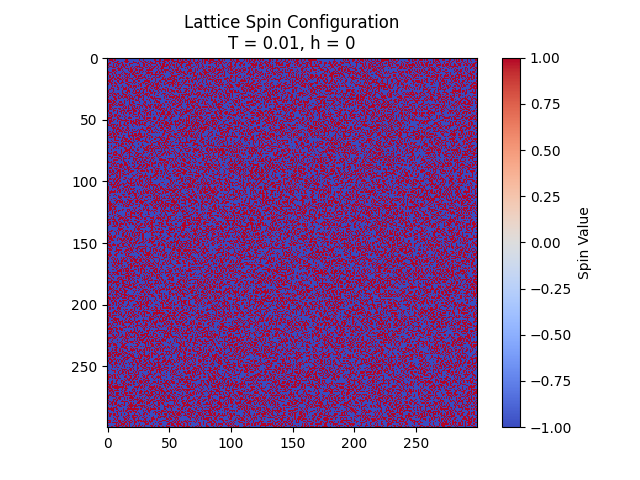
\includegraphics[width=0.7\textwidth]{nn, T=0.01, h=0.png}
    \captionof{figure}{output for low $T$ and $h=0$}
    \label{fig1}
\end{center}
 In Figure \eqref{fig1}, the amounts of blue points are slightly more than red points. It presents a disordered structure where infected and healthy people are randomly distributed.
 
2. Output for low $T$ and $h=100$
\begin{center}
\captionsetup{type=figure}
    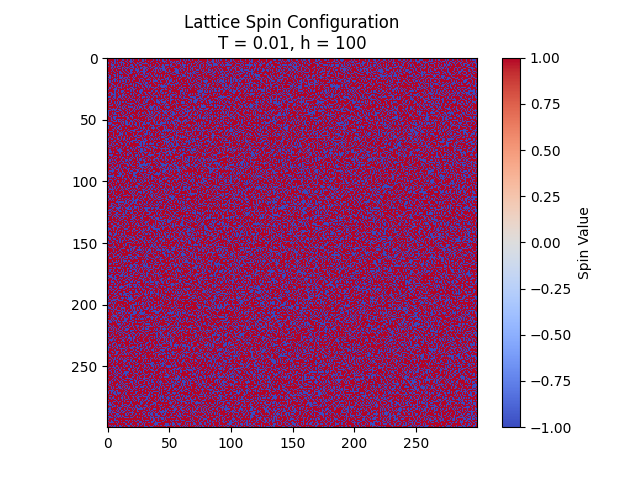
\includegraphics[width=0.7\textwidth]{nn, T=0.01, h=100.png}
    \captionof{figure}{output for low $T$ and $h=100$}
    \label{fig2}
\end{center}
Figure \eqref{fig2} is a disordered structure as well. However, compared to Figure \eqref{fig1}, Figure \eqref{fig2} contains a higher proportion of red spins. A possible cause of this is that the large value $h$ makes it difficult for the infected individuals to become immune.

3. Output for low $T$ and $h=-100$
\begin{center}
\captionsetup{type=figure}
    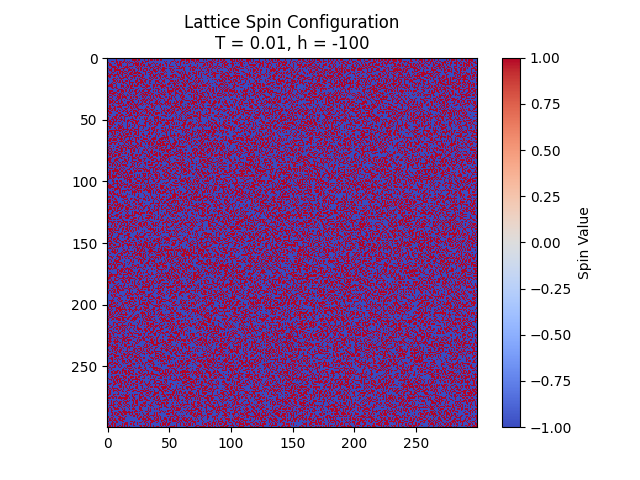
\includegraphics[width=0.7\textwidth]{nn, T=0.01, h=-100.png}
    \captionof{figure}{output for low $T$ and $h=-100$}
    \label{fig3}
\end{center}
Figure \eqref{fig3} is similar to Figure \eqref{fig1}. Both of them are disordered, with healthy people slightly more than infected people. Despite variations in the parameter $h$, the overall results remain largely unchanged. This suggests that the impact of $h$ may not be strong enough to counteract the effects of $T$ in this setting.

4. Output for high $T$ and $h=0$
\begin{center}
\captionsetup{type=figure}
    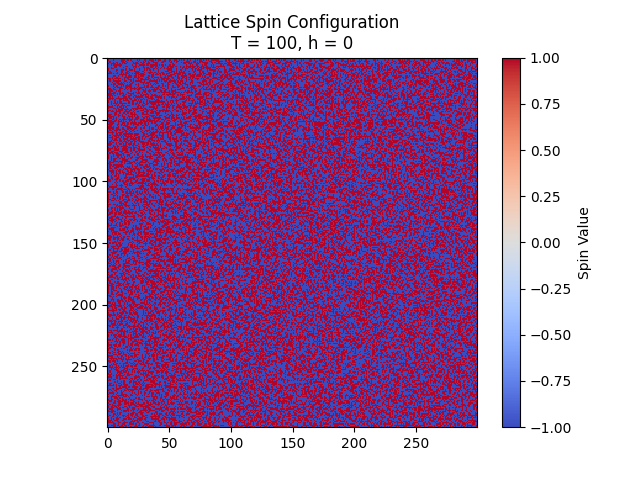
\includegraphics[width=0.7\textwidth]{nn, T=100, h=0.png}
    \captionof{figure}{output for high $T$ and $h=0$}
    \label{fig4}
\end{center}
In Figure \eqref{fig4}, the number of healthy and infected people are approximately equal. If we look at Figure \eqref{fig1} and \eqref{fig4} together, we can conclude that when $h=0$, both high $T$ and low $T$ present a disordered phase.

5. Output for high $T$ and $h=100$
\begin{center}
\captionsetup{type=figure}
    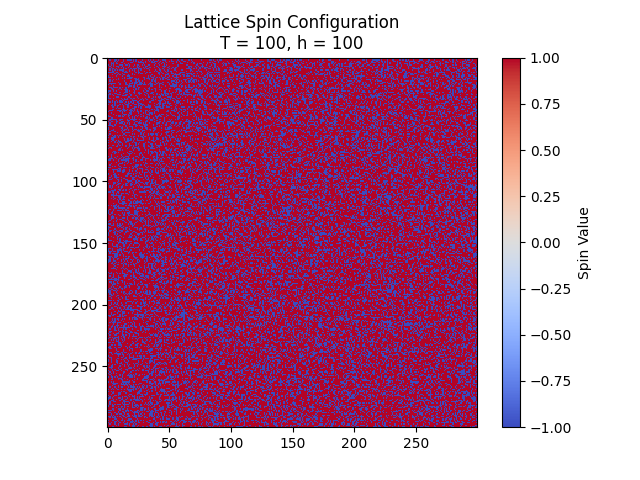
\includegraphics[width=0.7\textwidth]{nn, T=100, h=100.png}
    \captionof{figure}{output for high $T$ and $h=100$}
    \label{fig5}
\end{center}
Figure \eqref{fig5} presents a disordered phase with more infected people than healthy people. Compared with Figure \eqref{fig2}, the proportion of infected people is even higher. Thus, we can conclude that high $h$ weakens self-healing and high temperature promotes a more disordered structure.

6. Output for high $T$ and $h=-100$
\begin{center}
\captionsetup{type=figure}
    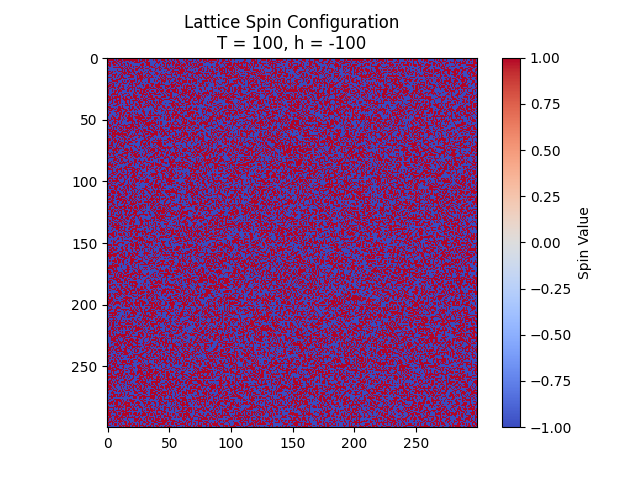
\includegraphics[width=0.7\textwidth]{nn, T=100, h=-100.png}
    \captionof{figure}{output for high $T$ and $h=-100$}
    \label{fig6}
\end{center}
Although Figure \eqref{fig6} is still disordered, it has more healthy people than Figure \eqref{fig5}. Here, high temperature again contributes to the disorder, but $h = -100$ strengthens the self-healing process, resulting in a greater number of healthy people.


We have also drawn two graphs displaying how the density of infected people varies with different values of $h$, under high $T$ and low $T$ respectively. In the graphs, the $x$-axis represents the values of $h$, and the $y$-axis denotes the density of infected individuals.

\begin{center}
\captionsetup{type=figure}
    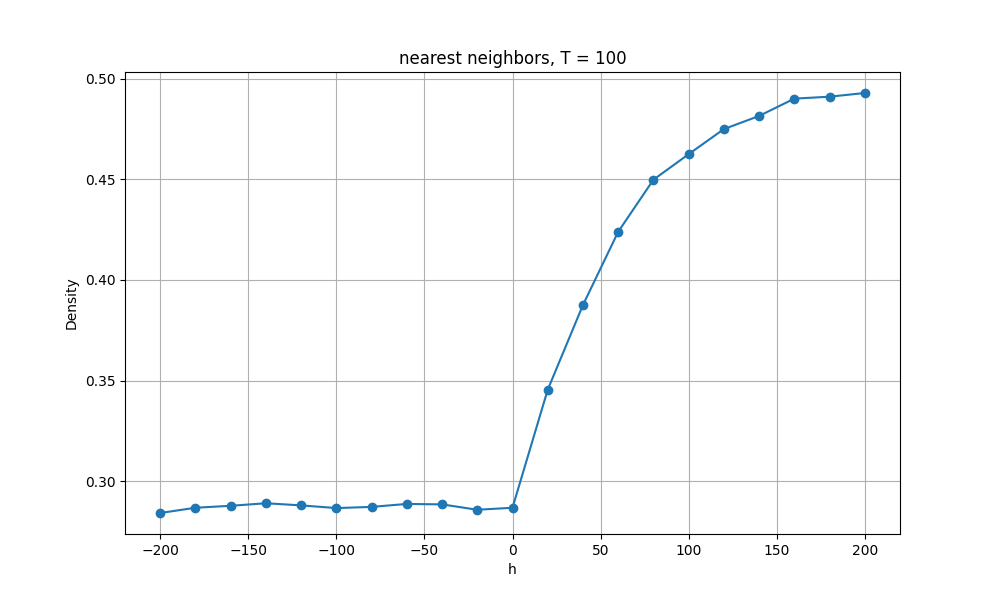
\includegraphics[width=0.7\textwidth]{nearest neighbors,T=100.jpg}
    \captionof{figure}{nearest neighbors, T=100}
    \label{fig7}
\end{center}


\begin{center}
\captionsetup{type=figure}
    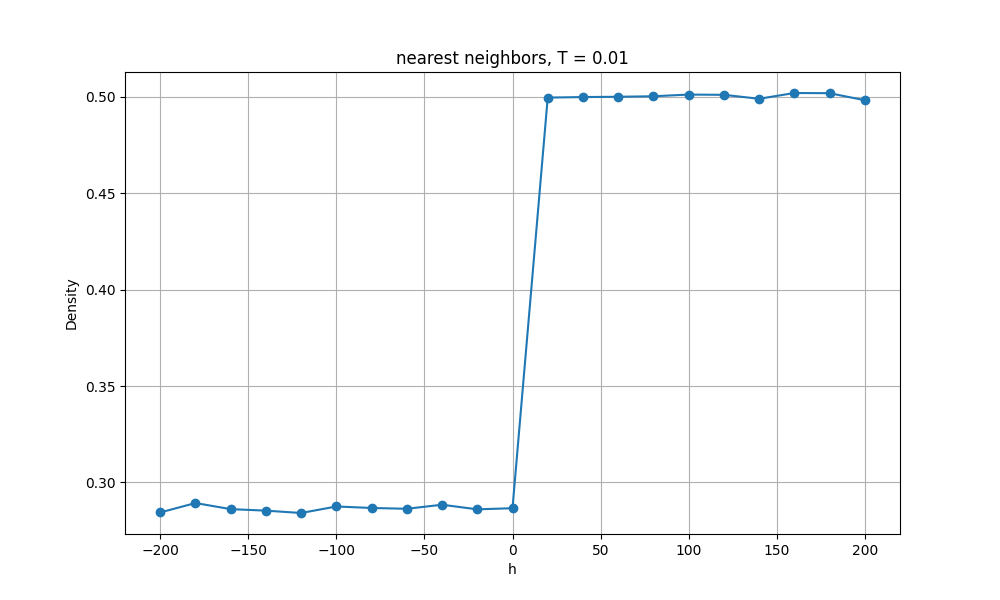
\includegraphics[width=0.7\textwidth]{nearest neighbors,T=0.01.jpg}
    \captionof{figure}{nearest neighbors, T=0.01}
    \label{fig8}
\end{center}

When $h < 0$, both the high $T$ and low $T$ graphs show a nearly constant density of approximately $0.275$. But when $h > 0$, the two graph exhibit differently: in the high $T$ scenario, as $h$ increases, the density seems to gradually converge to $0.5$; in the low $T$ scenario, as $h$ increases, there is a jump in density from $0.275$ to $0.5$ near 0. After that, it stabilizes near $0.5$.

\subsection{Long-Range}
In the long-range model, a selected spin can be influenced by other spins at a considerable distance, rather than being affected only by its four immediate neighbors. Here, $T$ retains its role from the Metropolis algorithm, where low $T$ leads to a higher correlation with other infected spins, and high $T$ results in greater independence. The parameter $a$ influences the value of $J$ in the model. In the subsequent graphs, we will examine the effects of varying $T$ and $a$.
\[
J_{x,y} = \frac{1}{(\left| x_1 - y_1 \right| + \left| x_2 - y_2 \right|)^a}
\]
Here $a$ is a parameter in this function to affect the value of $J_{x,y}$, and $x=(x_1,x_2)$ and $y=(y_1,y_2)$ are the points in the lattice. Note that we are using the 1-norm to calculate the distance between the points. In the following graphs we will also observe what is the behaviour of the density for different values of $T$ and $a$.

\subsubsection{Graph Analysis}

We will analyze the generated line graphs which presents the relationship between the value of $x$-axis $h$ (self-healing) and $y$-axis density. 
\begin{figure}
    \centering
    \begin{minipage}{0.45\textwidth}
        \centering
        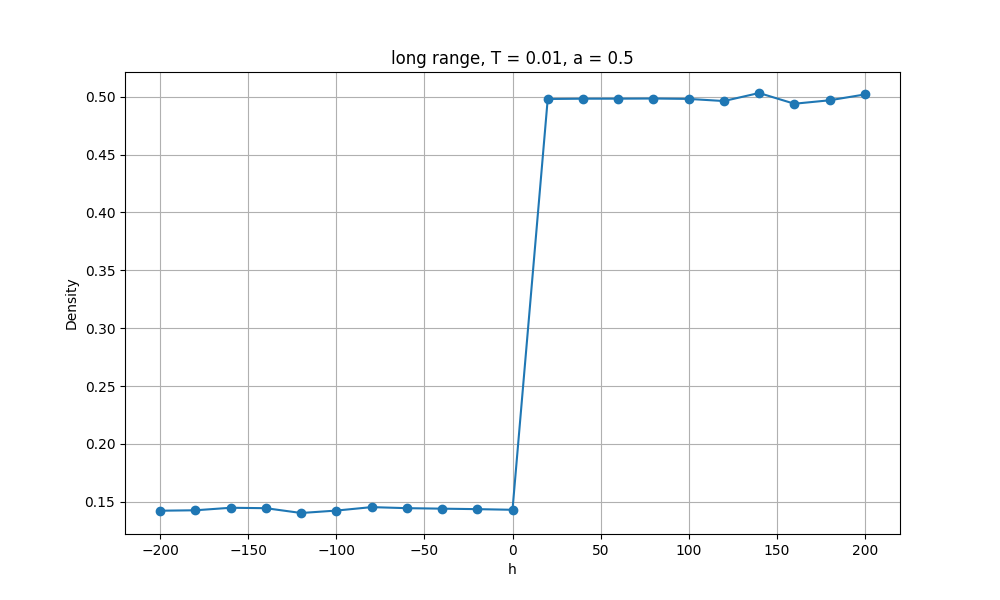
\includegraphics[width=0.9\textwidth]{long range,T=0.01,a=0.5.jpg} % first figure itself
        \caption{T=0.01, a=0.5}
        \label{fig9}
    \end{minipage}\hfill
    \begin{minipage}{0.45\textwidth}
        \centering
        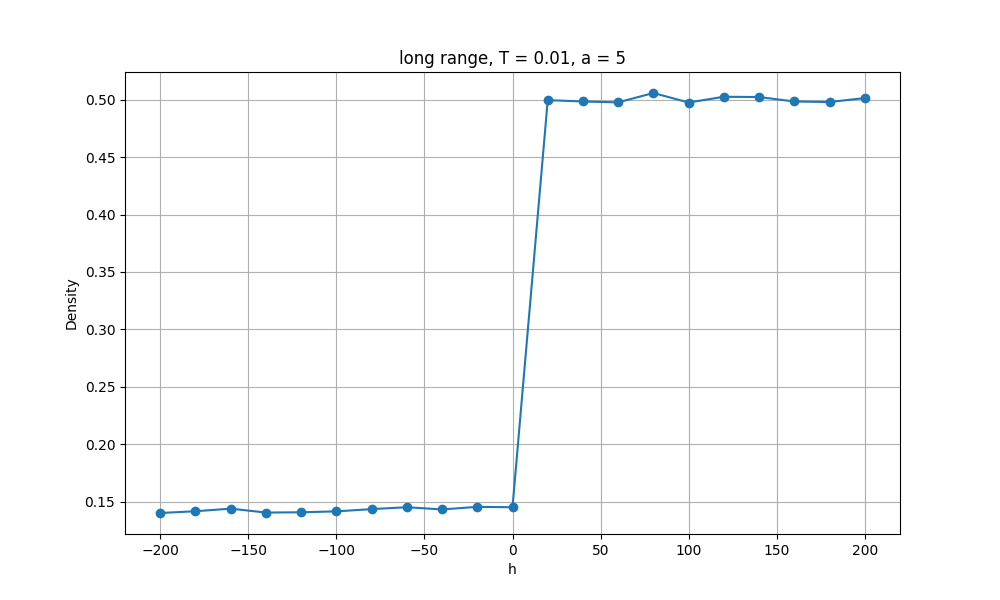
\includegraphics[width=0.9\textwidth]{long range,T=0.01,a=5.jpg} % second figure itself
        \caption{T=0.01, a=5}
        \label{fig10}
    \end{minipage}
\end{figure}

The two graphs presented in Figures \eqref{fig9} and \eqref{fig10} depict the density in the long-range model at low temperatures, with parameters $a = 0.5$ and $a = 5$. Both of them have a phase transition at $h=0$, and when $h<0$, the density stabilizes around the constant value of $0.15$, as for $h>0$, the density approaches a constant value of approximately $0.5$.

\begin{figure}
    \centering
    \begin{minipage}{0.45\textwidth}
        \centering
        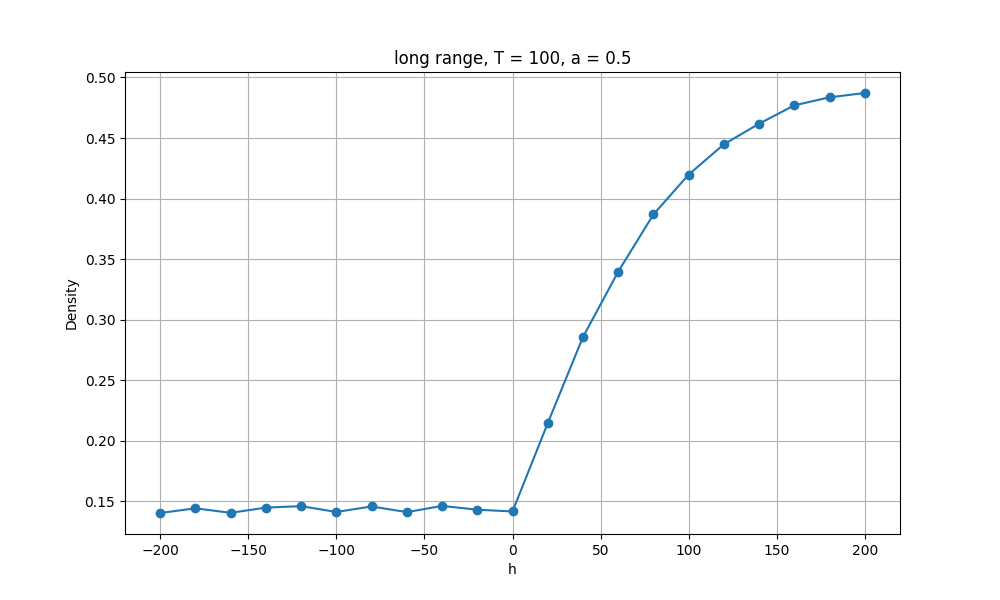
\includegraphics[width=0.9\textwidth]{long range,T=100,a=0.5.jpg} % first figure itself
        \caption{T=100, a=0.5}
        \label{fig11}
    \end{minipage}\hfill
    \begin{minipage}{0.45\textwidth}
        \centering
        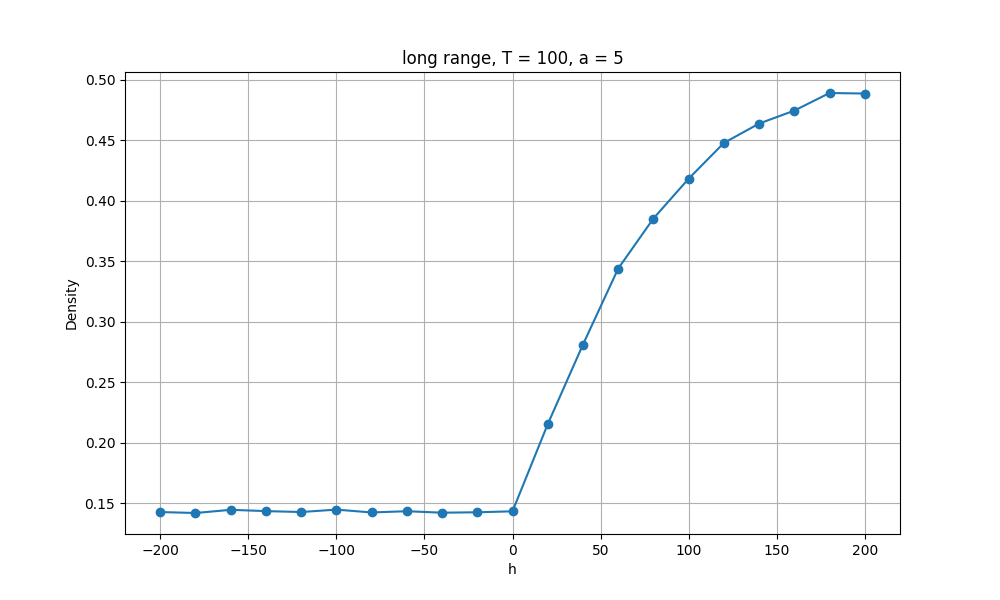
\includegraphics[width=0.9\textwidth]{long-range T=100, a=5.jpg} % second figure itself
        \caption{T=100, a=5}
        \label{fig12}
    \end{minipage}
\end{figure}

The Figures \eqref{fig11} and \eqref{fig12}, for $h < 0$, the density remains approximately constant at $0.15$, consistent with the behavior seen in Figures \eqref{fig9} and \eqref{fig10}. However, for $h > 0$, the density gradually converges to $0.5$, rather than undergoing an instantaneous change.

\subsubsection{Best-Fit Curve}

In this model, one of the noteworthy observations is that for large values of $h$, the density consistently converges to $0.5$. To quantitatively analyze this behavior, we applied the least-squares fitting method to determine the best-fit curve for the data obtained.

For this analysis, we focused on the long-range model with parameters $T = 100$ and $a = 5$. Based on our observations and underlying assumptions, we selected an exponential function as the most appropriate model to fit the curve.

\begin{center}
\captionsetup{type=figure}
    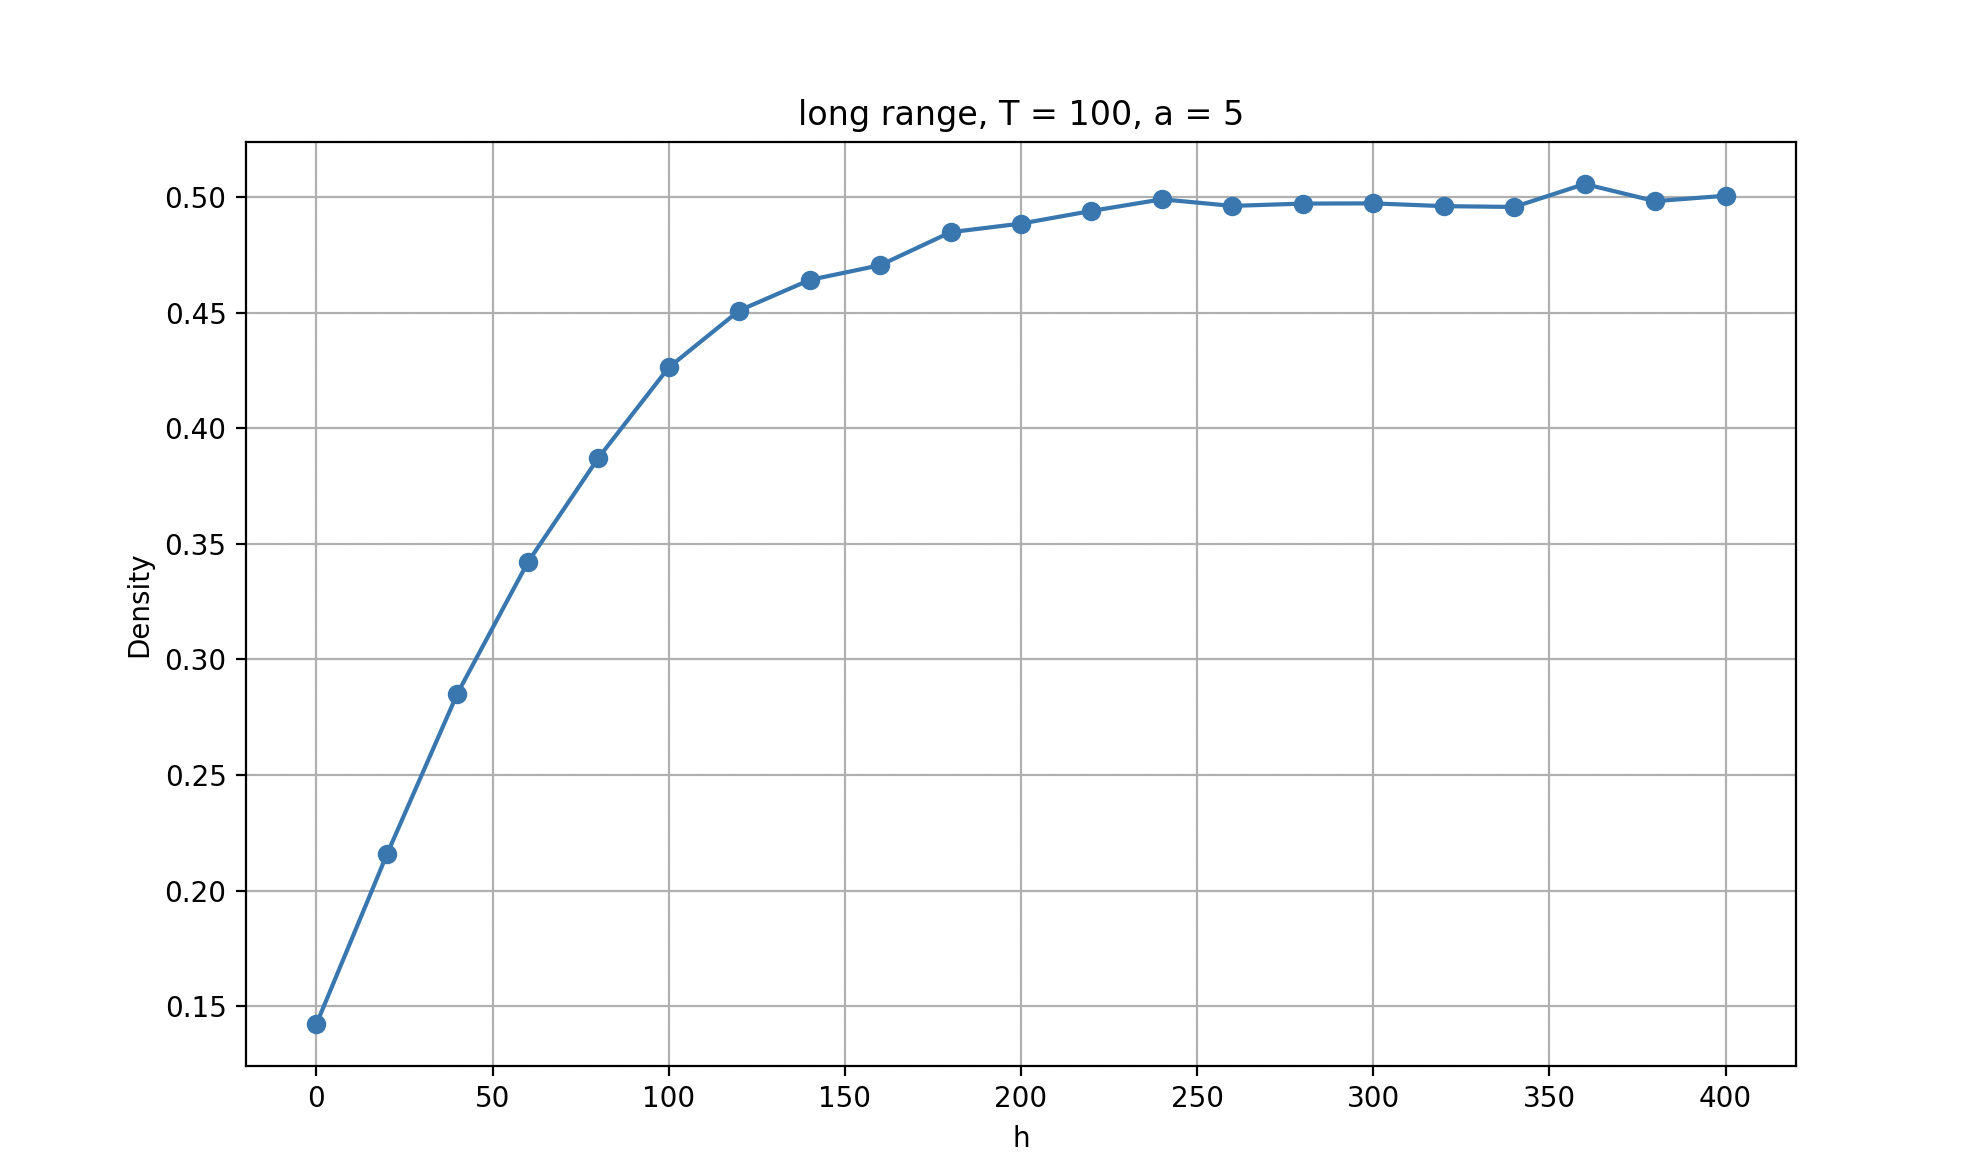
\includegraphics[width=0.7\textwidth]{long range T=100, a=5.jpg}
    \label{fig13}
\end{center}
This is the basic function model we use to fit
\begin{equation}\label{basic_function_model1}
y=\beta_1+\beta_2e^{-x}.
\end{equation}
Let $t=e^{-x}$, then we get
\begin{equation}\label{basic_function_model2}
    y=\beta_1+\beta_2t.
\end{equation}
Use the x-coordinates of the data to build the design matrix $X$ and the y-coordinates to build the observation vector $Y$, we can have
$$
X=
\begin{bmatrix}
    1&t_1\\
    1&t_2\\
\vdots&\vdots\\
    1&t_n\\
\end{bmatrix},
Y=
\begin{bmatrix}
y_1\\
y_2\\
\vdots\\
y_n
\end{bmatrix},
\beta=
\begin{bmatrix}
\beta_1\\
\beta_2
\end{bmatrix}.
$$
To solve for matrix $\beta$, we know that
\begin{equation}\label{best_fit}
X^TX\beta=X^TY,
\end{equation}
so here we get
$$
\begin{bmatrix}
    1&1&1&\dots&1\\
    t_1&t_2&t_3&\dots&t_n
\end{bmatrix}
\begin{bmatrix}
    1&t_1\\
    1&t_2\\
    1&t_3\\
    \vdots&\vdots\\
    1&t_n
\end{bmatrix}
\begin{bmatrix}
    \beta_1\\
    \beta_2
\end{bmatrix}
=\begin{bmatrix}
    y_1\\
    y_2\\
    \vdots\\
    y_n
\end{bmatrix}
\begin{bmatrix}
    1&1&1&\dots&1\\
    t_1&t_2&t_3&\dots&t_n. \\
\end{bmatrix}
$$
Then 
$
\begin{bmatrix}
\beta_1\\
\beta_2
\end{bmatrix}
$ can be presented as 
$$
\begin{bmatrix}
    \beta_1\\
    \beta_2
\end{bmatrix}
=(X^TX)^{-1}
\begin{bmatrix}
    y_1\\
    y_2\\
    \vdots\\
    y_n
\end{bmatrix}
\begin{bmatrix}
    1&1&1&\dots&1\\
    t_1&t_2&t_3&\dots&t_n
\end{bmatrix}.
$$
We use $21$ sets of data in our graphs here to fit the curve, which means $n=21$. The set of points is given by
\begin{align*}
\{ &(0, 0.142325), (20, 0.215675), (40, 0.2852), (60, 0.341975), \\
   &(80, 0.387075), (100, 0.426225), (120, 0.45085), (140, 0.464075), \\
   &(160, 0.47045), (180, 0.484725), (200, 0.48845), (220, 0.493925), \\
   &(240, 0.49895), (260, 0.4961), (280, 0.4971), (300, 0.4972), \\
   &(320, 0.496), (340, 0.49565), (360, 0.505575), (380, 0.49815), \\
   &(400, 0.5005) \}.
\end{align*}
Remember that when we calculate the data, we need to let $t=e^{-x}$.
Here we use the online least-square curve calculation \cite{curve} to help us get the result, which is
$$
\beta_1=0.4497, \beta_2=-0.307.
$$
Thus, the best-fit curve is
\begin{equation}\label{best_fit_curve}
y=0.4497-0.3074e^{-x}.
\end{equation}
To find the limit of this function,
\[
\lim_{x \to \infty} e^{-x} = 0.
\]
Therefore, the function \( y = 0.4497 - 0.3074e^{-x} \) approximately converges to $0.5$.


\subsection{Random Graph}
In the random graph model, we don't focus on the infection on 4 neighbors or long-distance spins in the lattice, but we can make connections among any vertices with walks in the graph. 

According to the formula, 
\[
H = -\sum_{x,y} \left( (\sum_{m = 1}^{k} A^m)[x, y] \right) \sigma_x \sigma_y.
\]

The parameter $k$ represents number of "walks" with a larger $k$ corresponding to a more extensive surrounding social circle. The parameter $p$ represents the probability of forming edges, which can be interpreted as the likelihood of identifying “potentially infected points.” A higher value of $p$ indicates a greater chance of establishing connections among vertices, thereby facilitating the spread of infection. The parameter $T$ remains indicative of the infection rate.

In this subsection, we will analyze the impact of varying values of $T,p,k$ in a group of three. For instance, by controlling the parameter $k$, we can specifically investigate the role of "walks" in the model.
\begin{figure}
    \centering
    \begin{minipage}{0.45\textwidth}
        \centering
        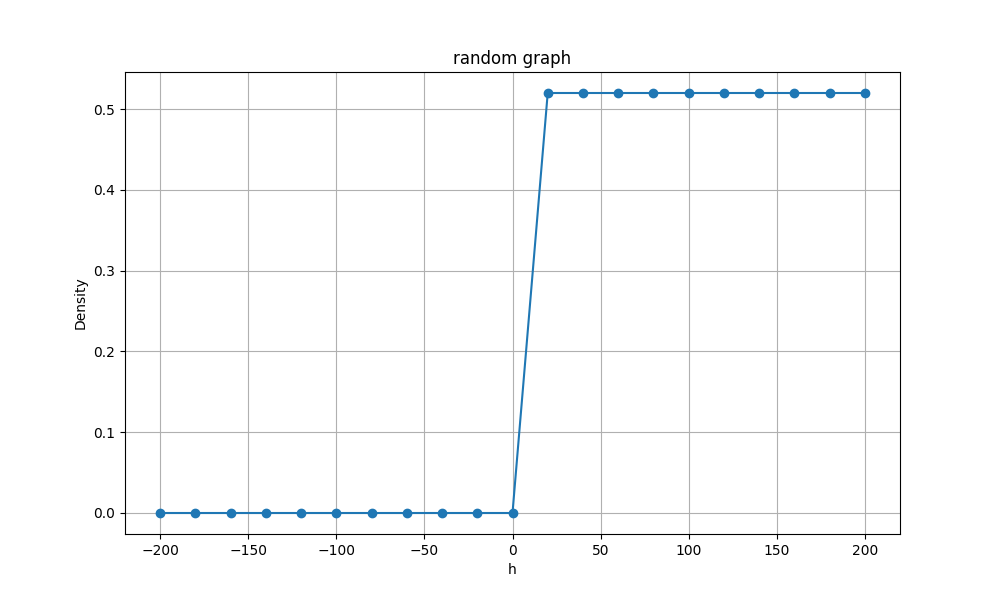
\includegraphics[width=0.9\textwidth]{rg.T=0.01,p=0.1,k=1.png} % first figure itself
        \caption{T=0.01, p=0.1, k=1}
        \label{fig14}
    \end{minipage}\hfill
    \begin{minipage}{0.45\textwidth}
        \centering
        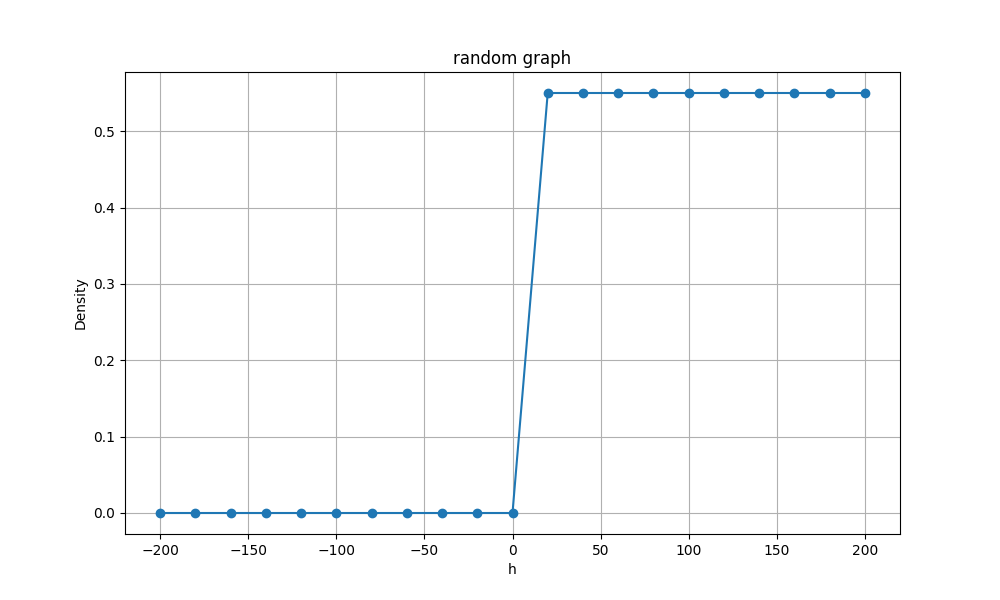
\includegraphics[width=0.9\textwidth]{rg.T=0.01, p=0.1 k=3.png} % second figure itself
        \caption{T=0.01, p=0.1, k=3}
        \label{fig15}
    \end{minipage}
    \begin{minipage}{0.45\textwidth}
        \centering
        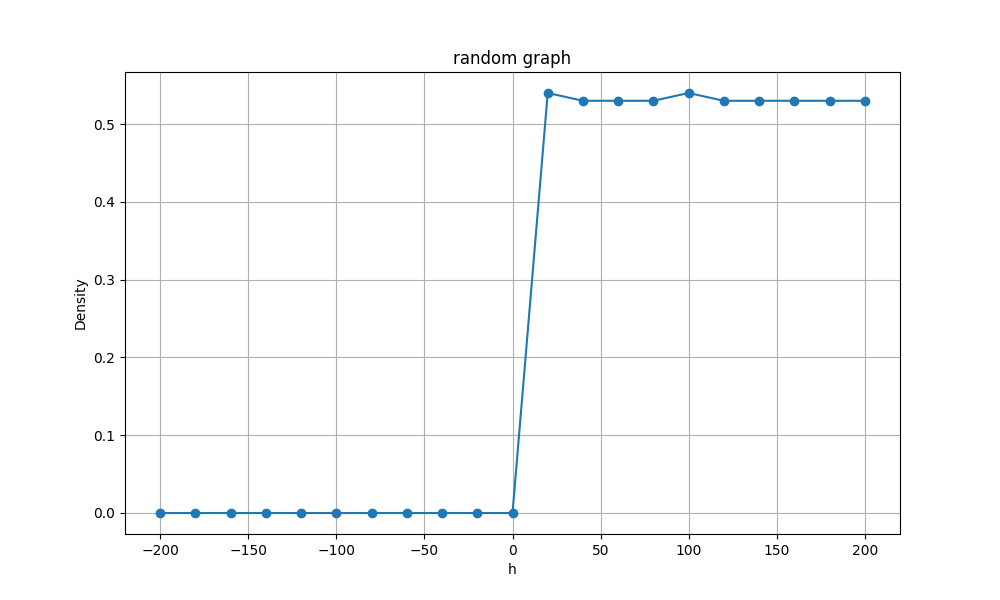
\includegraphics[width=0.9\textwidth]{rg.T=0.01, p=0.1 k=10.png} % first figure itself
        \caption{T=0.01, p=0.1, k=10}
        \label{fig16}
    \end{minipage}\hfill
\end{figure}
The first group is comprised of Figure \eqref{fig14}, Figure \eqref{fig15} and Figure \eqref{fig16}, with low $T$ and low $p$, which indicates more correlated infection, the low $p$ suggests a limited number of edges available for infection spread. We observe that each graph exhibits a phase transition at $h=0$. For $h < 0$, the density remains constant at $0$. However, for $h > 0$, the density approaches approximately $0.5$. Notably, with a low value of $k$, the density remains constant across the range of $h>0$. In contrast, for higher values of $k$, the density approaches $0.5$ when $h>0$, though it does not remain constant.


\begin{figure}
    \centering
    \begin{minipage}{0.45\textwidth}
        \centering
        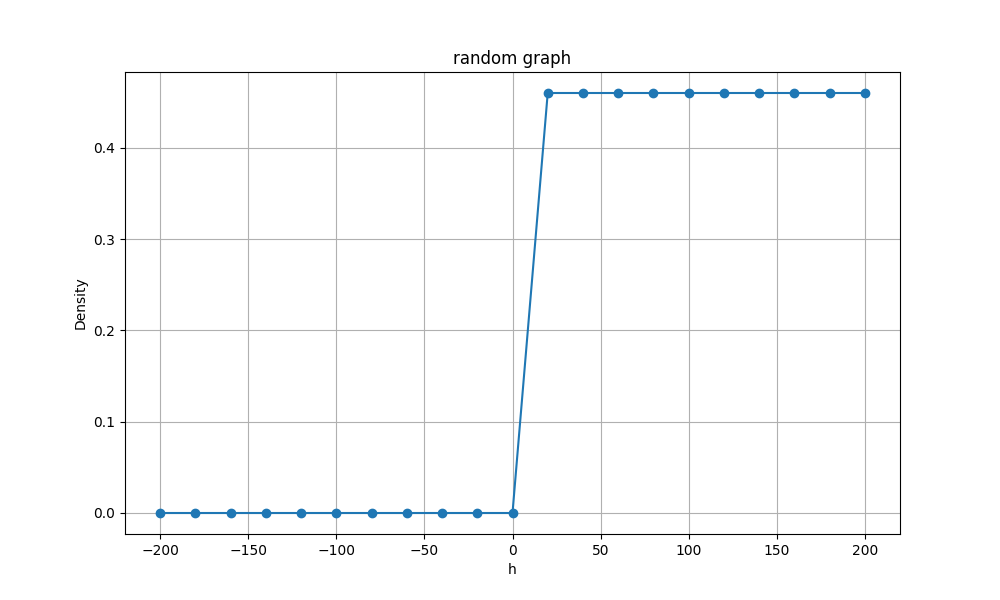
\includegraphics[width=0.9\textwidth]{rg. T=0.01, p=0.9 k=1.png} % first figure itself
        \caption{T=0.01, p=0.9, k=1}
        \label{fig17}
    \end{minipage}\hfill
    \begin{minipage}{0.45\textwidth}
        \centering
        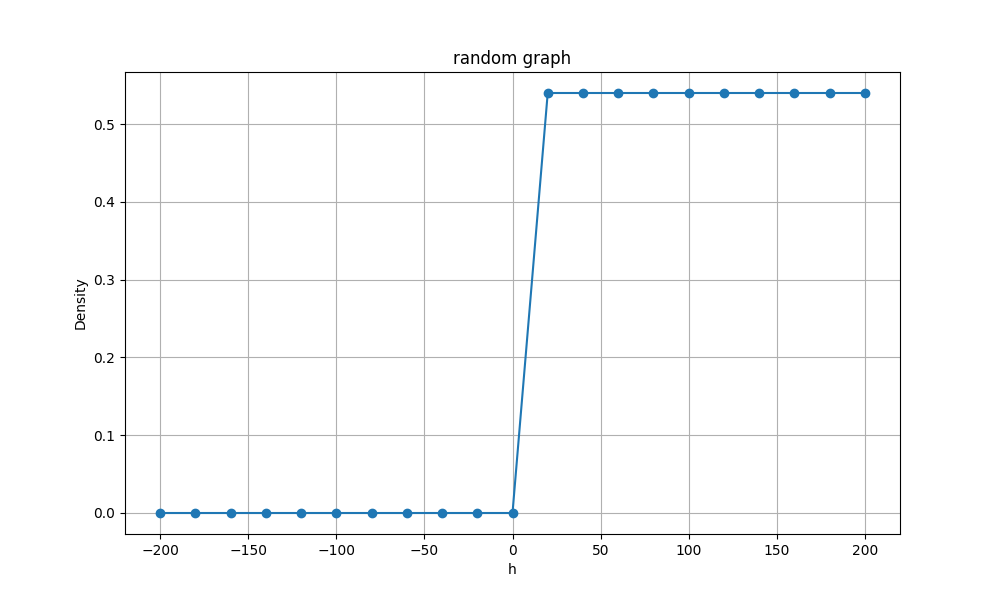
\includegraphics[width=0.9\textwidth]{rg. T=0.01 p=0.9 k=3.png} % second figure itself
        \caption{T=0.01, p=0.9, k=3}
        \label{fig18}
    \end{minipage}
    \begin{minipage}{0.45\textwidth}
        \centering
        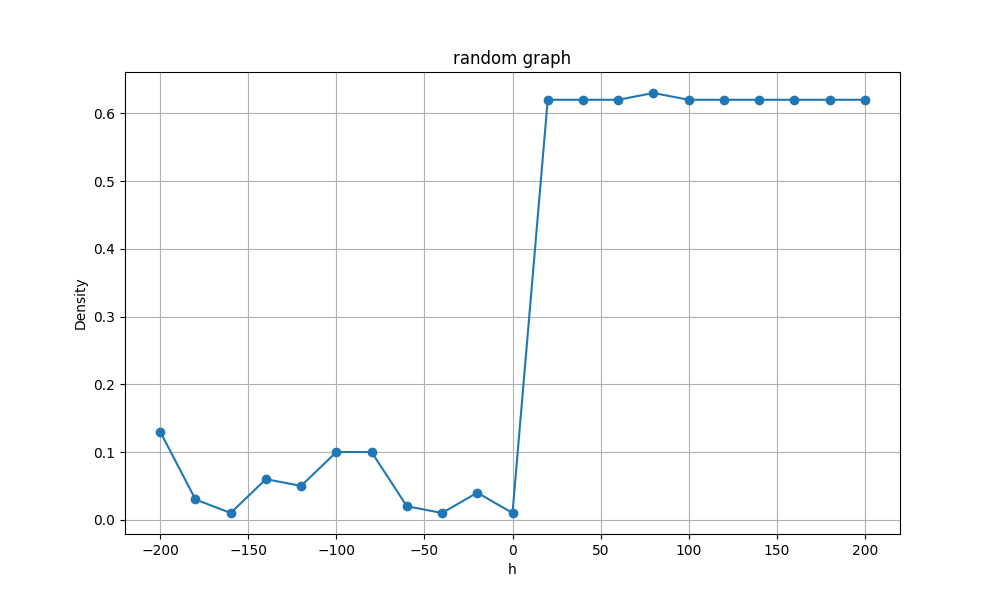
\includegraphics[width=0.9\textwidth]{rg. T=0.01 p=0.9 k=10.png} % first figure itself
        \caption{T=0.01, p=0.9, k=10}
        \label{fig19}
    \end{minipage}\hfill
\end{figure}
Figures \eqref{fig17}, \eqref{fig18}, and \eqref{fig19} also exhibit a phase transition at $h=0$, similar to the previous set of graphs. When $k$ is low, negative values of $h$ result in a density that remains constant at $0$. However, with higher values of $k$, negative $h$ leads to a non-constant density, which appears as a broken line. Additionally, across all three graphs, when $h$ is positive, the density stabilizes around $0.5$ for low $k$, while for high $k$, it stabilizes around $0.6$.

\begin{figure}
    \centering
    \begin{minipage}{0.45\textwidth}
        \centering
        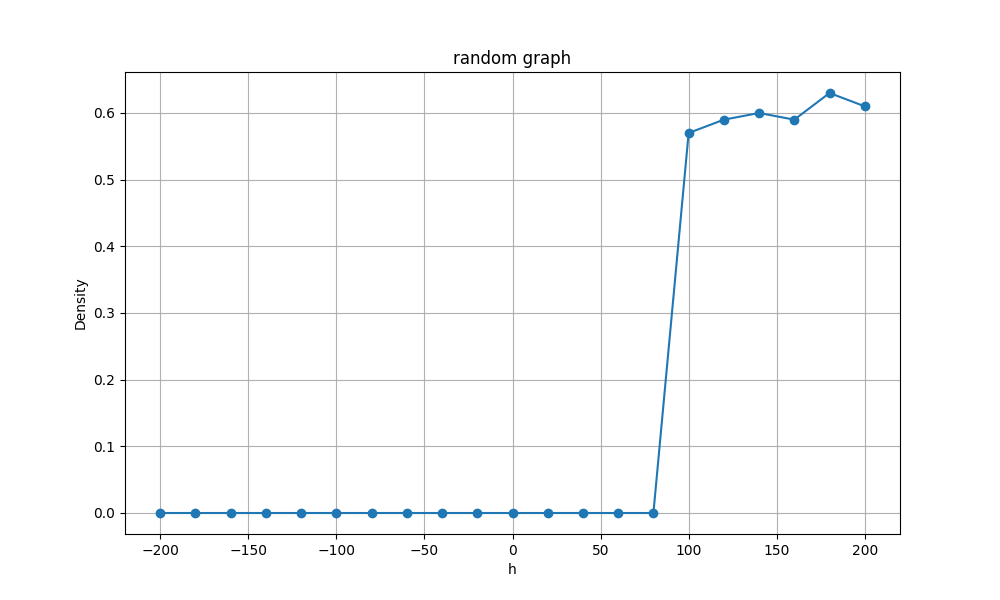
\includegraphics[width=0.9\textwidth]{rg.T=100,p=0.5,k=1.png} % first figure itself
        \caption{T=100, p=0.5, k=1}
        \label{fig20}
    \end{minipage}\hfill
    \begin{minipage}{0.45\textwidth}
        \centering
        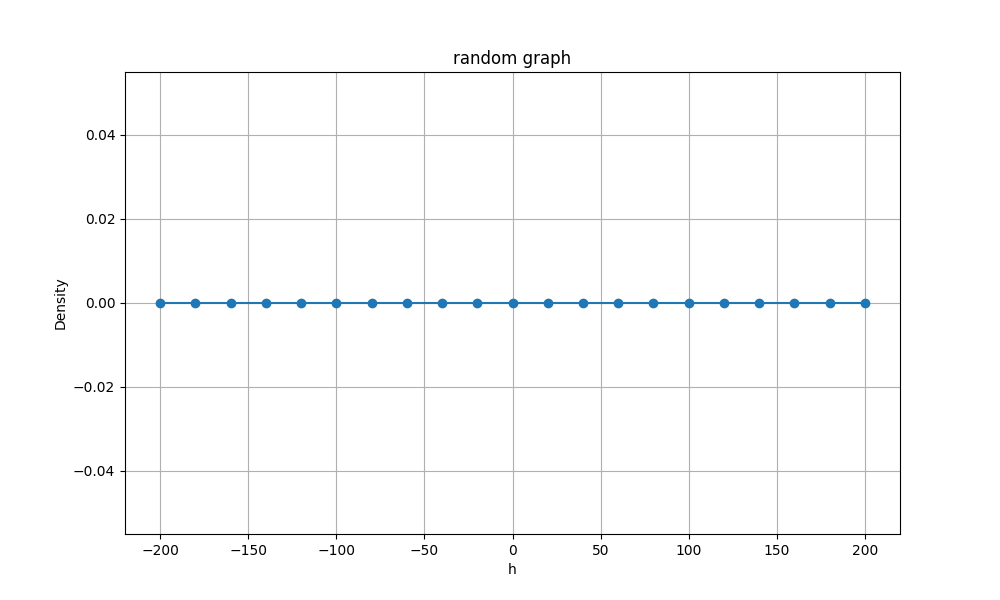
\includegraphics[width=0.9\textwidth]{rg.T=100 p=0.5 k=3.png} % second figure itself
        \caption{T=100, p=0.5, k=3}
        \label{fig21}
    \end{minipage}
    \begin{minipage}{0.45\textwidth}
        \centering
        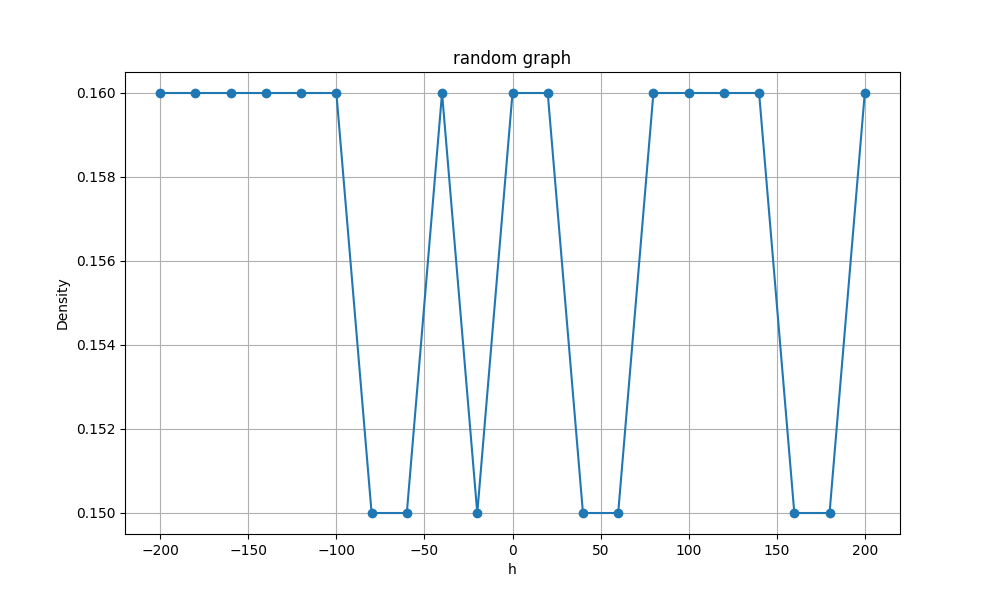
\includegraphics[width=0.9\textwidth]{rg.T=100, p=0.5, k=10.png} % first figure itself
        \caption{T=100, p=0.5, k=10}
        \label{fig22}
    \end{minipage}\hfill
\end{figure}

Figures \eqref{fig20}, \eqref{fig21}, and \eqref{fig22} illustrate the graphs with high $T$, $p=0.5$, and varying values of $k$. Unlike the previous cases, these graphs do not exhibit similar patterns. Specifically, when $T=100$, $p=0.5$, and $k=3$, the density remains constantly at $0$. In contrast, when $k=1$, a phase transition occurs, and for $k=10$, the density stabilizes around $0.15$ to $0.16$.

\begin{figure}
    \centering
    \begin{minipage}{0.45\textwidth}
        \centering
        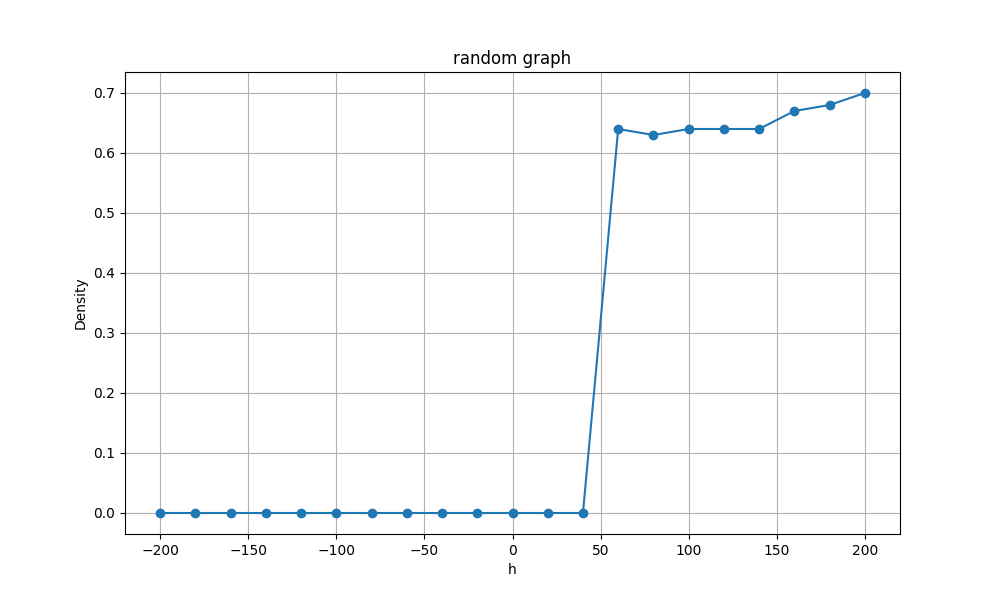
\includegraphics[width=0.9\textwidth]{rg. T=100, p=0.1, k=1.png} % first figure itself
        \caption{T=100, p=0.1, k=1}
        \label{fig23}
    \end{minipage}\hfill
    \begin{minipage}{0.45\textwidth}
        \centering
        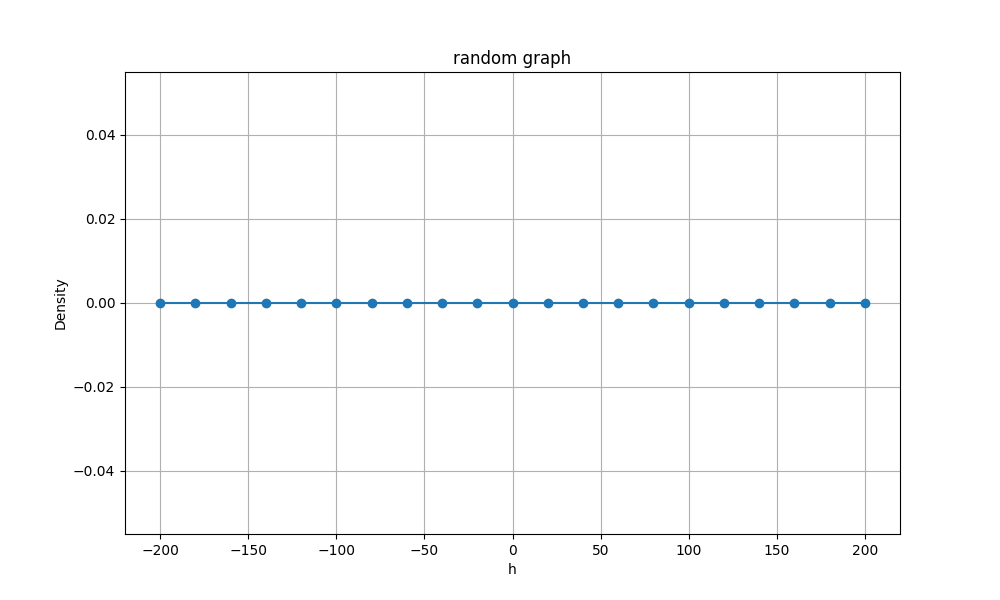
\includegraphics[width=0.9\textwidth]{rg. T=100,p=0.1,k=3.png} % second figure itself
        \caption{T=100, p=0.1, k=3}
        \label{fig24}
    \end{minipage}
    \begin{minipage}{0.45\textwidth}
        \centering
        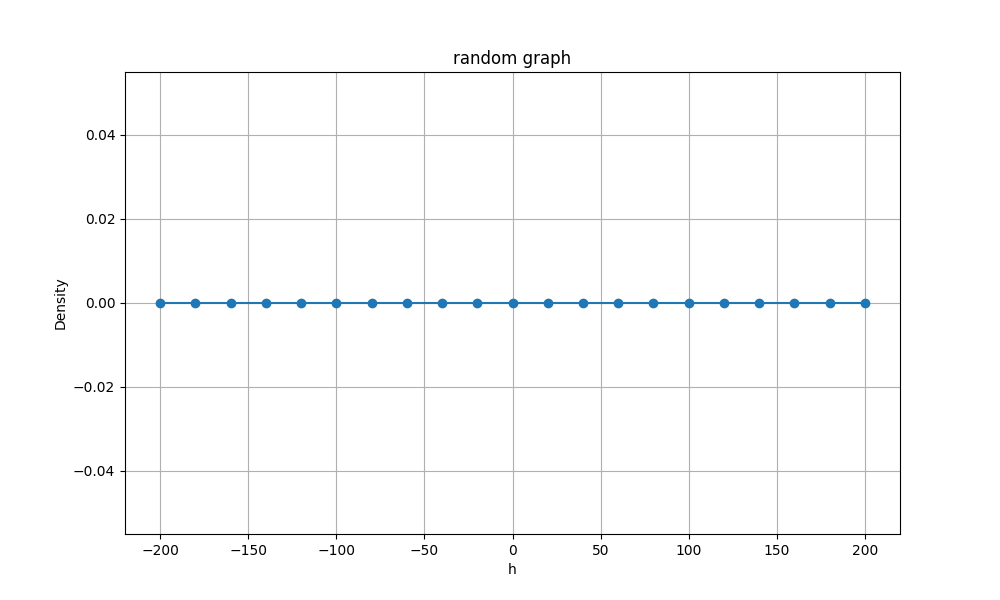
\includegraphics[width=0.9\textwidth]{rg.T=100, p=0.1 k=10.png} % first figure itself
        \caption{T=100, p=0.1, k=10}
        \label{fig25}
    \end{minipage}\hfill
\end{figure}

Figures \eqref{fig23}, \eqref{fig24}, and \eqref{fig25} depict the graphs under conditions of high $T$ and low $p$. For $k=3$ and $k=10$, the density remains constant at $0$. However, when $k=1$, a phase transition is observed around $h=50$.

\begin{figure}
    \centering
    \begin{minipage}{0.45\textwidth}
        \centering
        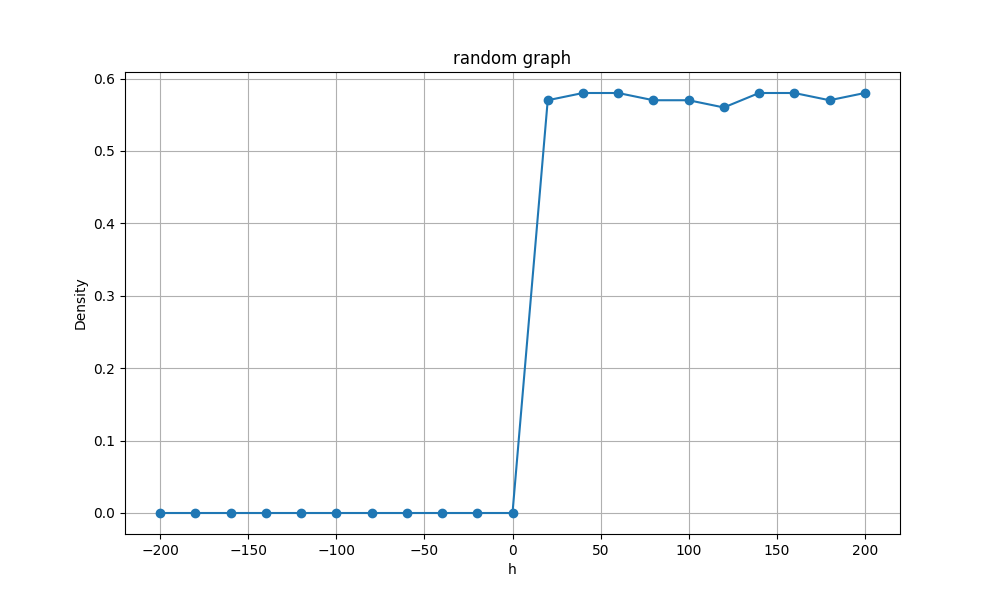
\includegraphics[width=0.9\textwidth]{rg_T=0.01,p=0.5,k=1.png} % first figure itself
        \caption{T=0.01, p=0.5, k=1}
        \label{fig26}
    \end{minipage}\hfill
    \begin{minipage}{0.45\textwidth}
        \centering
        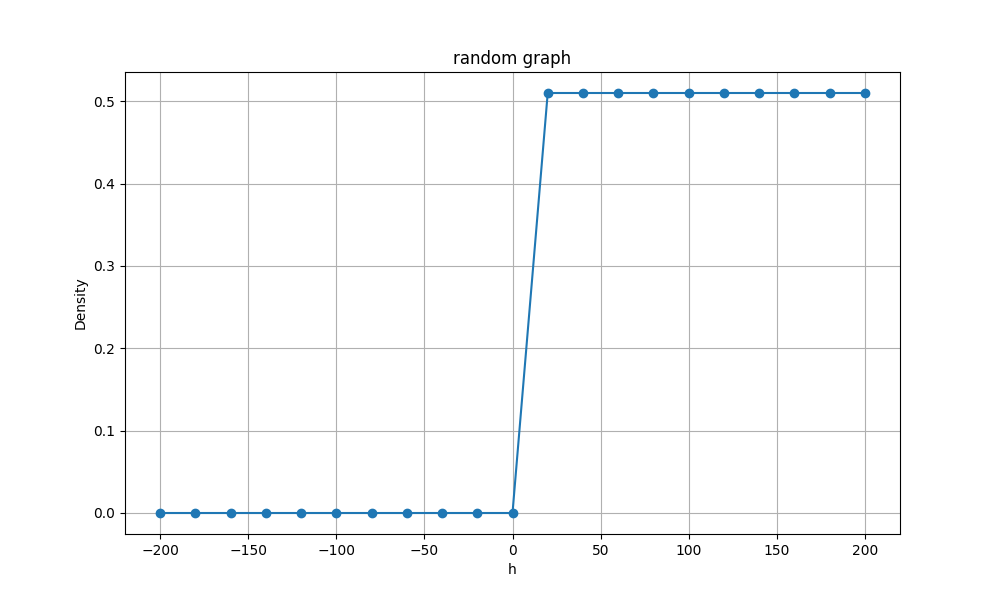
\includegraphics[width=0.9\textwidth]{rg,T=0.01,p=0.5,k=3.png} % second figure itself
        \caption{T=0.01, p=0.5, k=3}
        \label{fig27}
    \end{minipage}
    \begin{minipage}{0.45\textwidth}
        \centering
        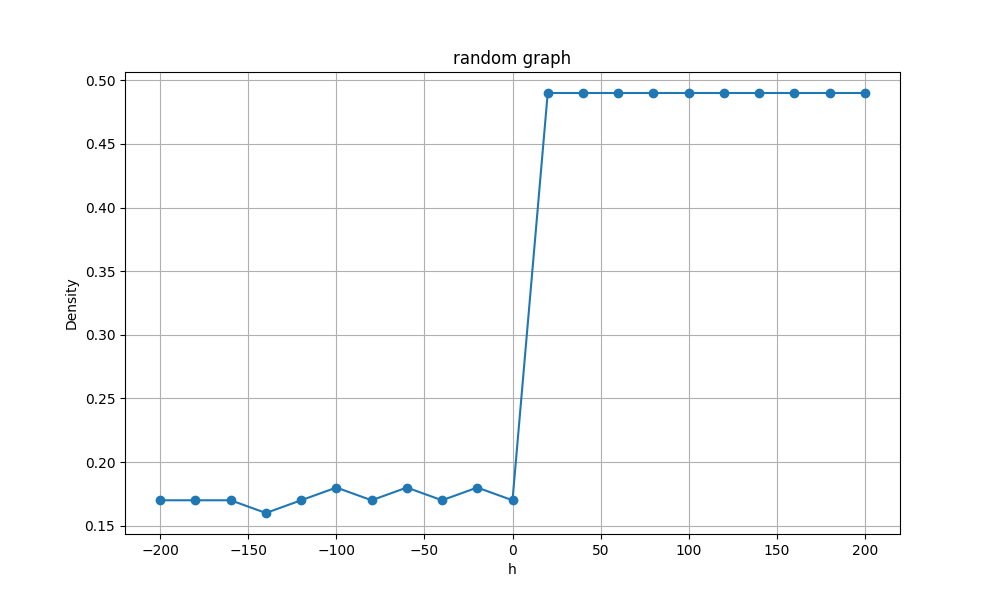
\includegraphics[width=0.9\textwidth]{rg,T=0.01,p=0.5,k=10.png} % first figure itself
        \caption{T=0.01, p=0.5, k=10}
        \label{fig28}
    \end{minipage}\hfill
\end{figure}

Figures \eqref{fig26}, \eqref{fig27}, and \eqref{fig28} all present a phase transition at $h=0$. At low values of $k$, the density is approximately $0$ when $h<0$, and it increases to around $0.5 \sim 0.6$ when $h>0$. Interestingly, for higher values of $k$, the density becomes less stable around $0.15$ when $h< 0$, while it stabilizes at a constant value of $0.5$ when $h>0$. Conversely, for low $k$, the density is less stable at positive $h$ and remains constant at negative $h$.

\begin{figure}
    \centering
    \begin{minipage}{0.45\textwidth}
        \centering
        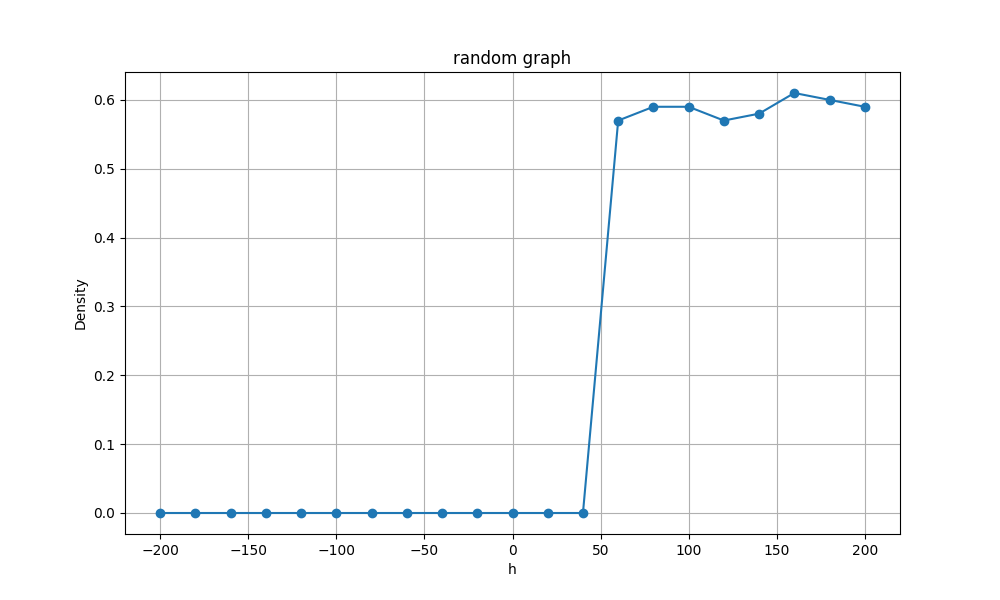
\includegraphics[width=0.9\textwidth]{rg,T=100,p=0.9,k=1.png} % first figure itself
        \caption{T=100, p=0.9, k=1}
        \label{fig29}
    \end{minipage}\hfill
    \begin{minipage}{0.45\textwidth}
        \centering
        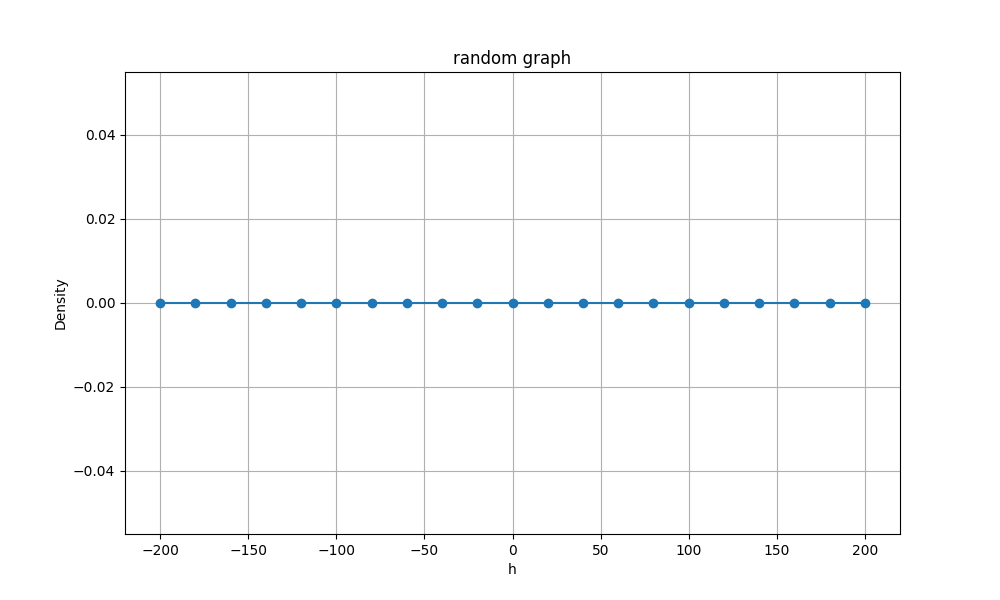
\includegraphics[width=0.9\textwidth]{rg. T=100, p=0.9, k=3.png} % second figure itself
        \caption{T=100, p=0.9, k=3}
        \label{fig30}
    \end{minipage}
    \begin{minipage}{0.45\textwidth}
        \centering
        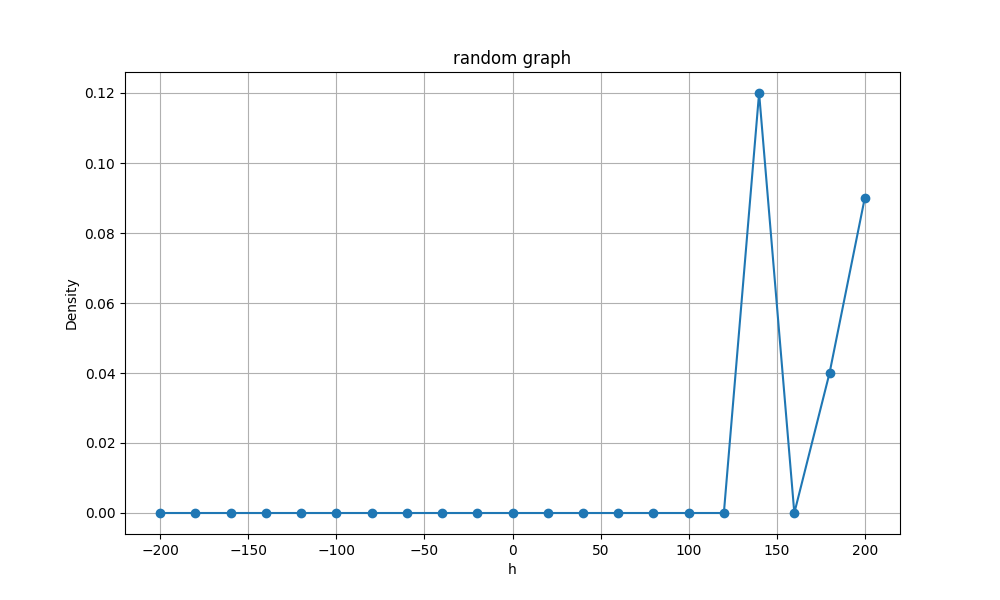
\includegraphics[width=0.9\textwidth]{rg,T=100,p=0.9,k=10.png} % first figure itself
        \caption{T=100, p=0.9, k=10}
        \label{fig31}
    \end{minipage}\hfill
\end{figure}

Figures \eqref{fig29}, \eqref{fig30}, and \eqref{fig31} all show a constant density of $0$ when $h$ is negative. In the graph with low $k$, a phase transition occurs around $h=50$, and for $h>50$, the density stabilizes around $0.6$. When $k=3$, the density remains consistently at $0$. In Figure \eqref{fig30}, a phase transition occurs at approximately $h=120$; for $h<120$, the density stays constant at $0$. Notably, although it can be an issue from the capacity of the algorithm, around $h=160$, the density briefly returns to $0$ before increasing again.

\chapter{Codes in Python}

The inspiration of our codes come from an exercise provided by the project “Ayomide A Bamidele - 2016/PHY236\_2016” \cite{Bamidele}, which helped us build the Metropolis algorithm for the 2D Ising model. Based on our intuition and creative ideas, we then developed three new models of our own: the nearest-neighbors model, the long-range model, and the random-graph model, offering different perspectives for analyzing the infection process.

\section{The Nearest-Neighbors Model}

Let's imagine that on a 2D plane, we have an $N \times M$ grid. A person stands on each grid point, and the distance between two people is counted by the number of sides between them. In the nearest-neighbors model, we assume that the status of a point only depends on the four points which are one side away from it. We can easily picture that the four points are respectively on the left, on the right, at the top and in the bottom, which look like the closest neighbors to the selected point. This is why we name it as the nearest-neighbors model.

Now, let's go through the functions one by one.

\begin{figure}
    \centering
    
\includegraphics[width=1\linewidth]{nn_randomLattice.png}
    \caption{\texttt{randomLattice(N, M)}}
    \label{fig40}
\end{figure}

\subsection{\texttt{randomLattice(N, M)}}

This function aims to generate an $N \times M$ matrix, where each entry is randomly assigned with $\pm 1$. To ensure the randomness, we use the built-in function called \texttt{np.random.choice($[-1, 1]$)}.

\begin{figure}
    \centering
    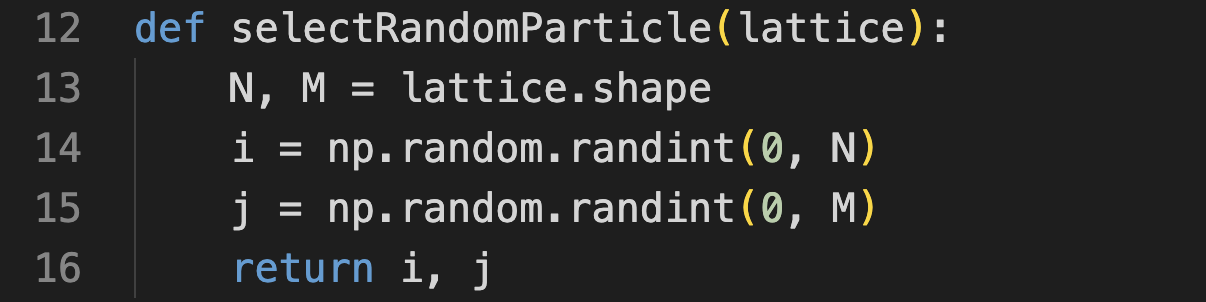
\includegraphics[width=1\linewidth]{nn_selectRandomParticle.png}
    \caption{\texttt{selectRandomParticle(lattice)}}
    \label{fig41}
\end{figure}

\subsection{\texttt{selectRandomParticle(lattice)}}

In this function, we want to select a point randomly. Since all points in the lattice are in the form of ordered number pairs $(i, j)$, we select a point by generating random values of $i$ and $j$. We should note that $i \in [0, N)$,  $j \in [0, M)$.

\begin{figure}
    \centering
    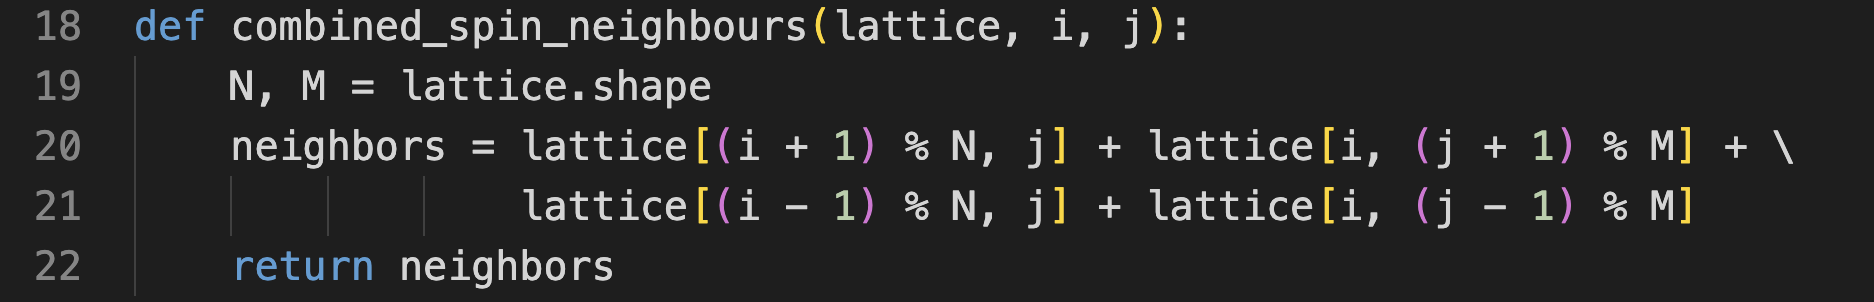
\includegraphics[width=1\linewidth]{nn_combined_spin_neighbors.png}
    \caption{\texttt{combinedSpinNeighbors(lattice, i, j)}}
    \label{fig42}
\end{figure}

\subsection{\texttt{combinedSpinNeighbors(lattice, i, j)}}

In this function, let's calculate the sum of the selected point's nearest neighbors. To do that, we need to find the values of the four neighbors separately and then add them together. From the previous function, we have randomly selected a point, $(i, j)$, whose value should be lattice$[i, j]$. We know that $i$ represents the row and $j$ represents the column, and the lattice has $N$ rows and $M$ columns. As an example, let's try to find the value of the point's right neighbor. Compared with the selected point, its right neighbor is on the same row but one column to the right, so its value should be lattice$[i, j + 1]$. However, if the selected point is on column $M - 1$, which is the right border of the whole lattice, this expression would be erroneous. Therefore, let's make it a rule that if a point is on the right border of the lattice, its right neighbor should be the point in the same row, but on the left border of the lattice (column $0$). Therefore, 
\[
lattice[i, (j + 1) \mod M]
\]
is the correct expression of the right neighbor of any selected point. Similarly, we can get the expressions of the point's left neighbor, top neighbor and bottom neighbor, which respectively are $lattice[i, (j - 1) \mod M]$, $lattice[(i - 1) \mod N, j]$, and $lattice[(i + 1) \mod N, j]$. Finally, we add these values together and get the sum of the nearest neighbors of the selected point.

\begin{figure}
    \centering
    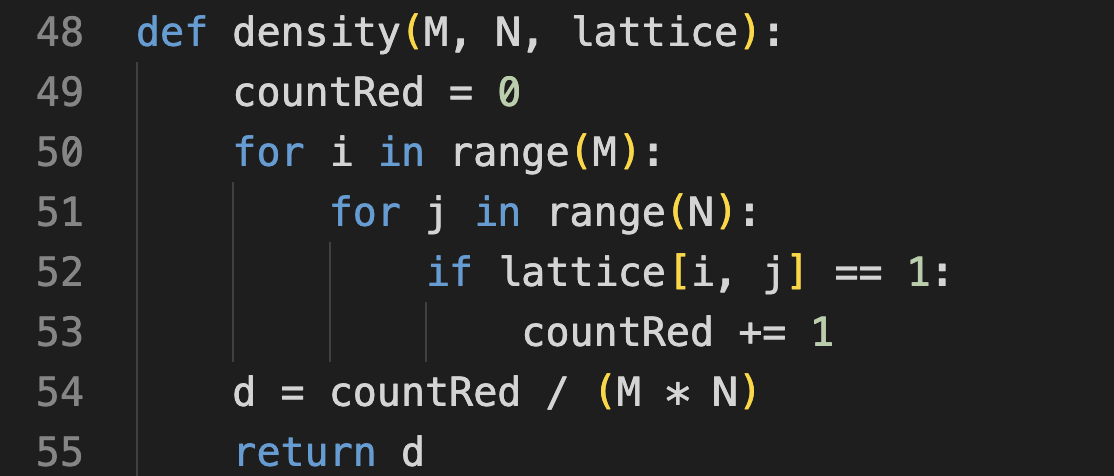
\includegraphics[width=1\linewidth]{nn_densityOfRed.png}
    \caption{\texttt{density(M, N, lattice)}}
    \label{fig43}
\end{figure}

\subsection{\texttt{density(M, N, lattice)}}

This function calculates the density of red points, which stands for the density of the infected population. We use a nested for-loop to iterate over all points in the lattice. If the point is red, we add 1 to the total amount of red points. Finally, we divide the total amount of red points by the amount of all points to get the density of the red.

\begin{figure}
    \centering
    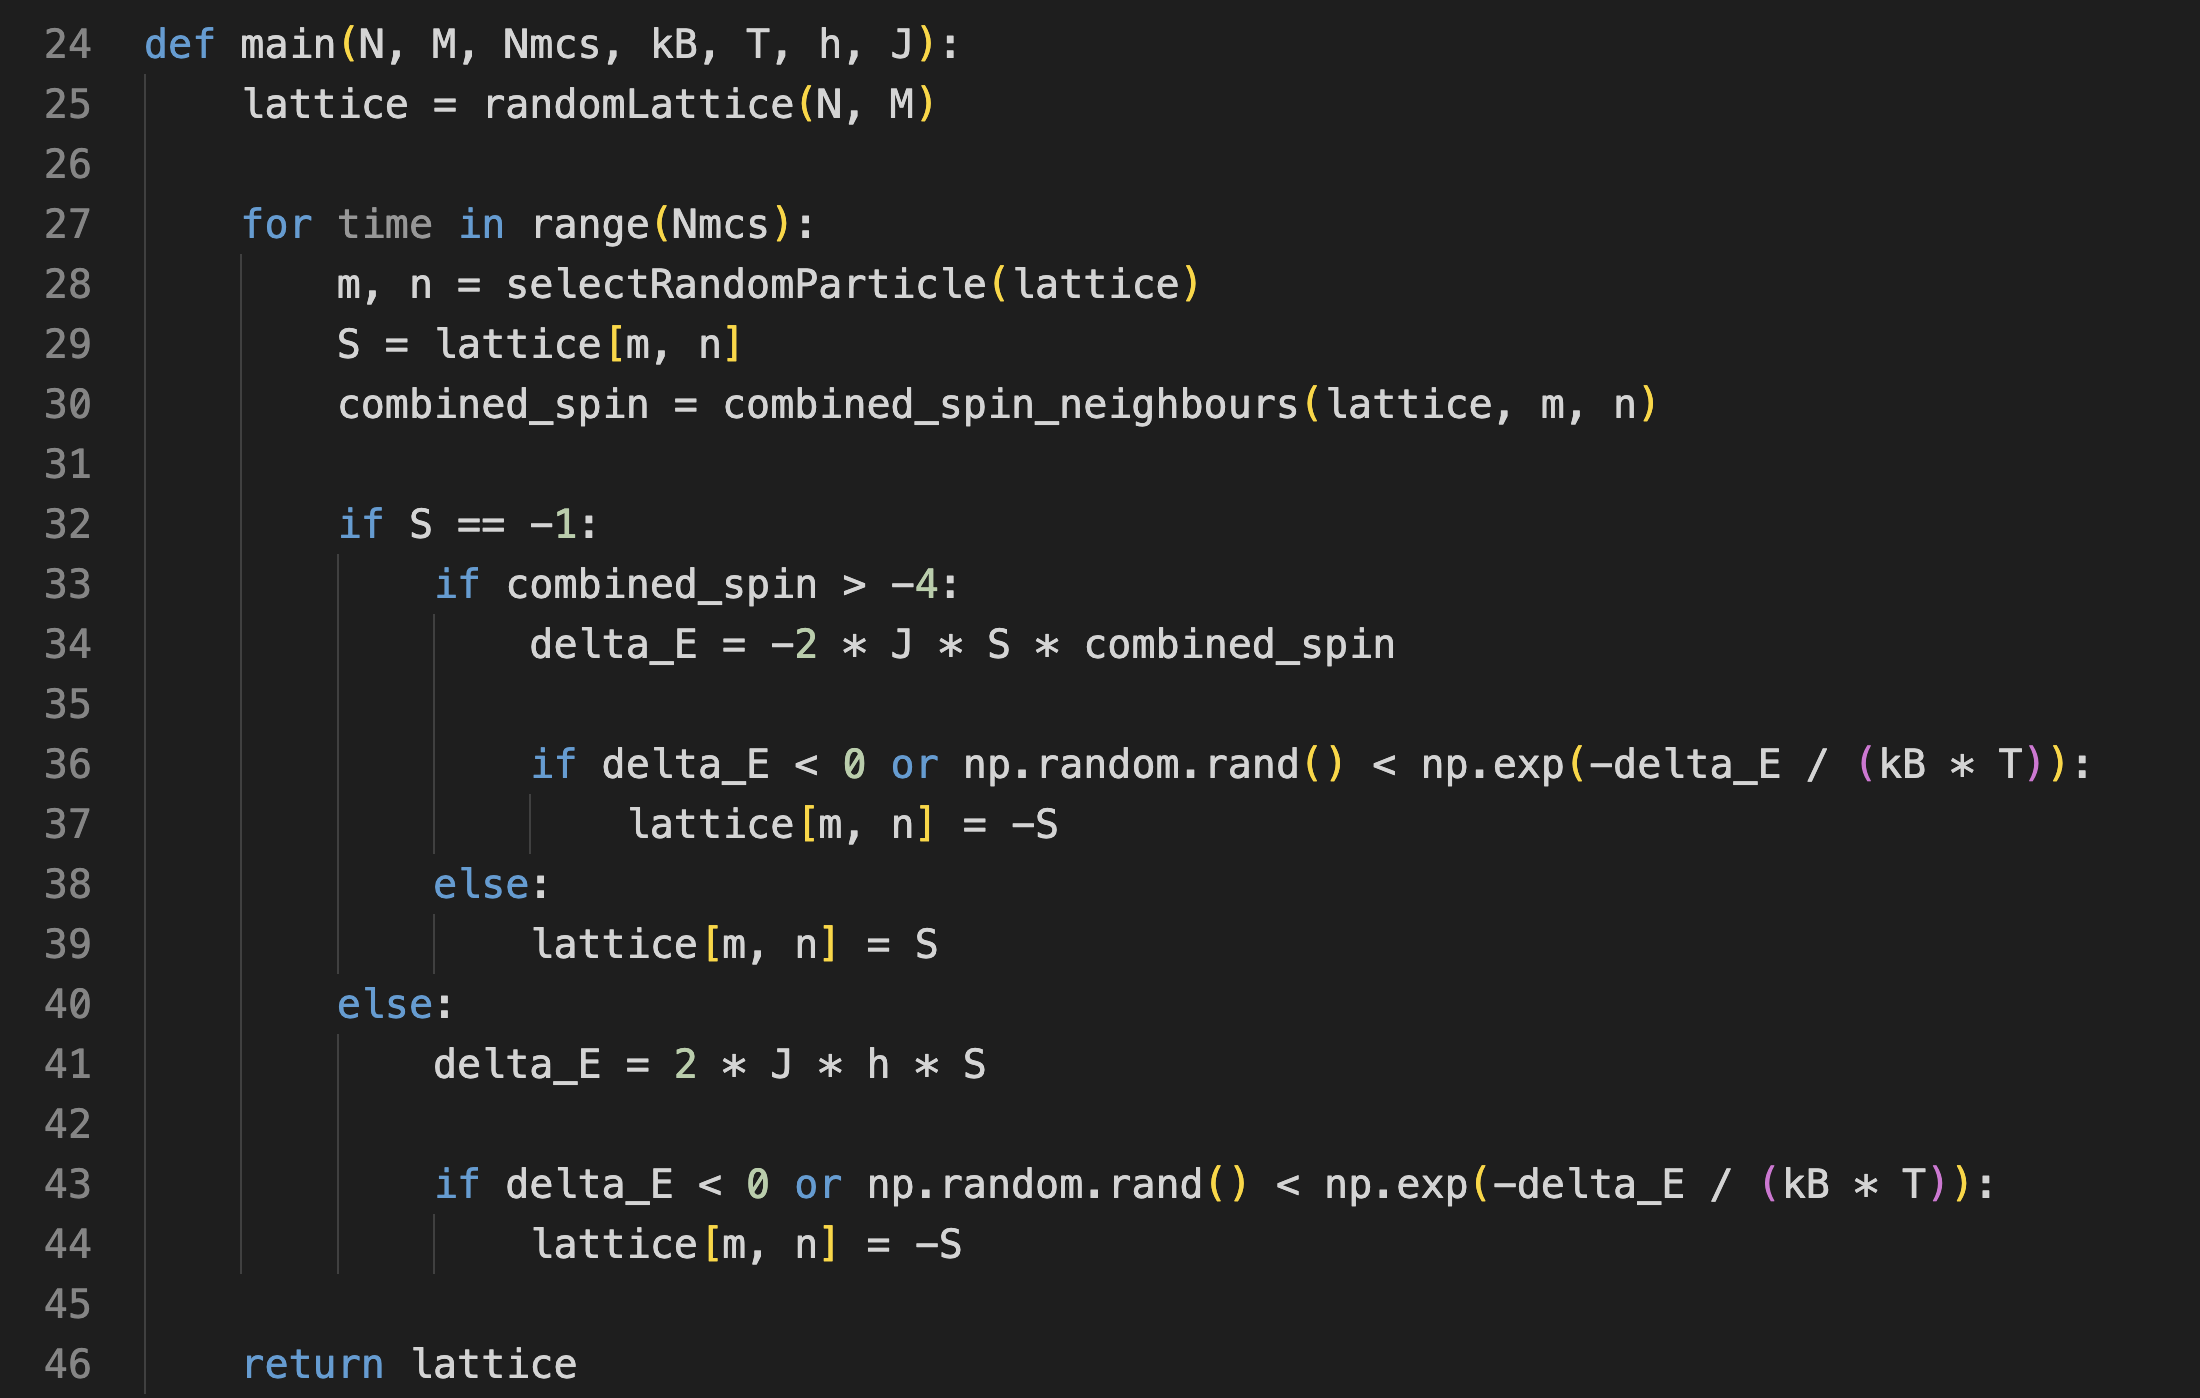
\includegraphics[width=1\linewidth]{nn_main.png}
    \caption{\texttt{main(N, M, Nmcs, kB, T, h, J)}}
    \label{fig44}
\end{figure}

\subsection{\texttt{main(N, M, Nmcs, kB, T, h, J)}}

Now we finally arrive at the most critical part, the main function. We would like to describe the logic of the function through the following bullet points.

\begin{enumerate}
\item[(1)] First, we generate a random lattice with points randomly set to be $1$ or $-1$. This lattice simulates the distribution of a group of people, where each point represents a person and $1$ or $-1$ indicates if the person is ill or healthy.
\item[(2)] Next, we write an outer iteration which counts the times of the Monte Carlo process.
\item[(3)] Then in each iteration, we randomly select a point in the lattice. $S$ is the corresponding value of the point.
\item[(4)] Since $S$ can be either $1$ or $-1$, it leads to two different occasions: First, let’s consider $S$ to be $-1$, indicating that the selected person is healthy. Now, if the sum of its nearest neighbors is $-4$, it suggests that all of its neighbors are healthy. It would be unreasonable if the person still has some risk to be infected. Therefore, we keep the value of $S$. However, if the sum is bigger than $-4$, some of its neighbors are ill, so there certainly is some possibility for the person to be infected, and we follow the metropolis algorithm to decide whether or not to flip the value of $S$. The metropolis algorithm goes like this:
\begin{enumerate}
\item[(4.1)] First, we calculate $\Delta E = 2 * H$, where $H$ is obtained by $-J * S *$ sum-of-the-nearest-neighbors.
\item[(4.2)] If $\Delta E$ is smaller than 0, we flip $S$.
\item[(4.3)] If $\Delta E$ is larger than 0, we need to further generate a random number $\mu$ between 0 and 1, and calculate $Z = e^{\frac{\Delta E}{kB \cdot T}}$. And now, we have two more occasions. If $\mu < Z$, we flip the value of S. Else, if $\mu > Z$, we keep the value of S.
\end{enumerate}
\item[(5)] Now let’s consider $S = 1$. In this situation, we need to follow the metropolis algorithm with border conditions. We should first calculate $\Delta E = -2 * J * S * h$. Then, similar to (4.2) and (4.3), only when $\Delta E < 0$ or $\mu < Z$ do we flip $S$. Otherwise, we keep the value of $S$.
\item[(6)] Finally, after the times of the Monte Carlo process reach $Nmcs$, we return the lattice.
\end{enumerate}

\subsection{Calling the Functions}

Now that we have all the functions we need, let's puzzle them together. First, we should assign values to the parameters $N, M, Nmcs, kB, h, T, J$. Let's recall that $N$ and $M$ stands for the number of rows and columns of the lattice; $Nmcs$ is the times of the Monte Carlo Process; $kB$ is the Boltzmann constant; $T$ is the temperature; and $J$ is exchange interaction constant. Next, we call the main function to get the final lattice. Then we call the  density function to get a numerical view of the distribution of infected people. Finally, we can plot a graph of the density to $h$.

\begin{figure}
    \centering
    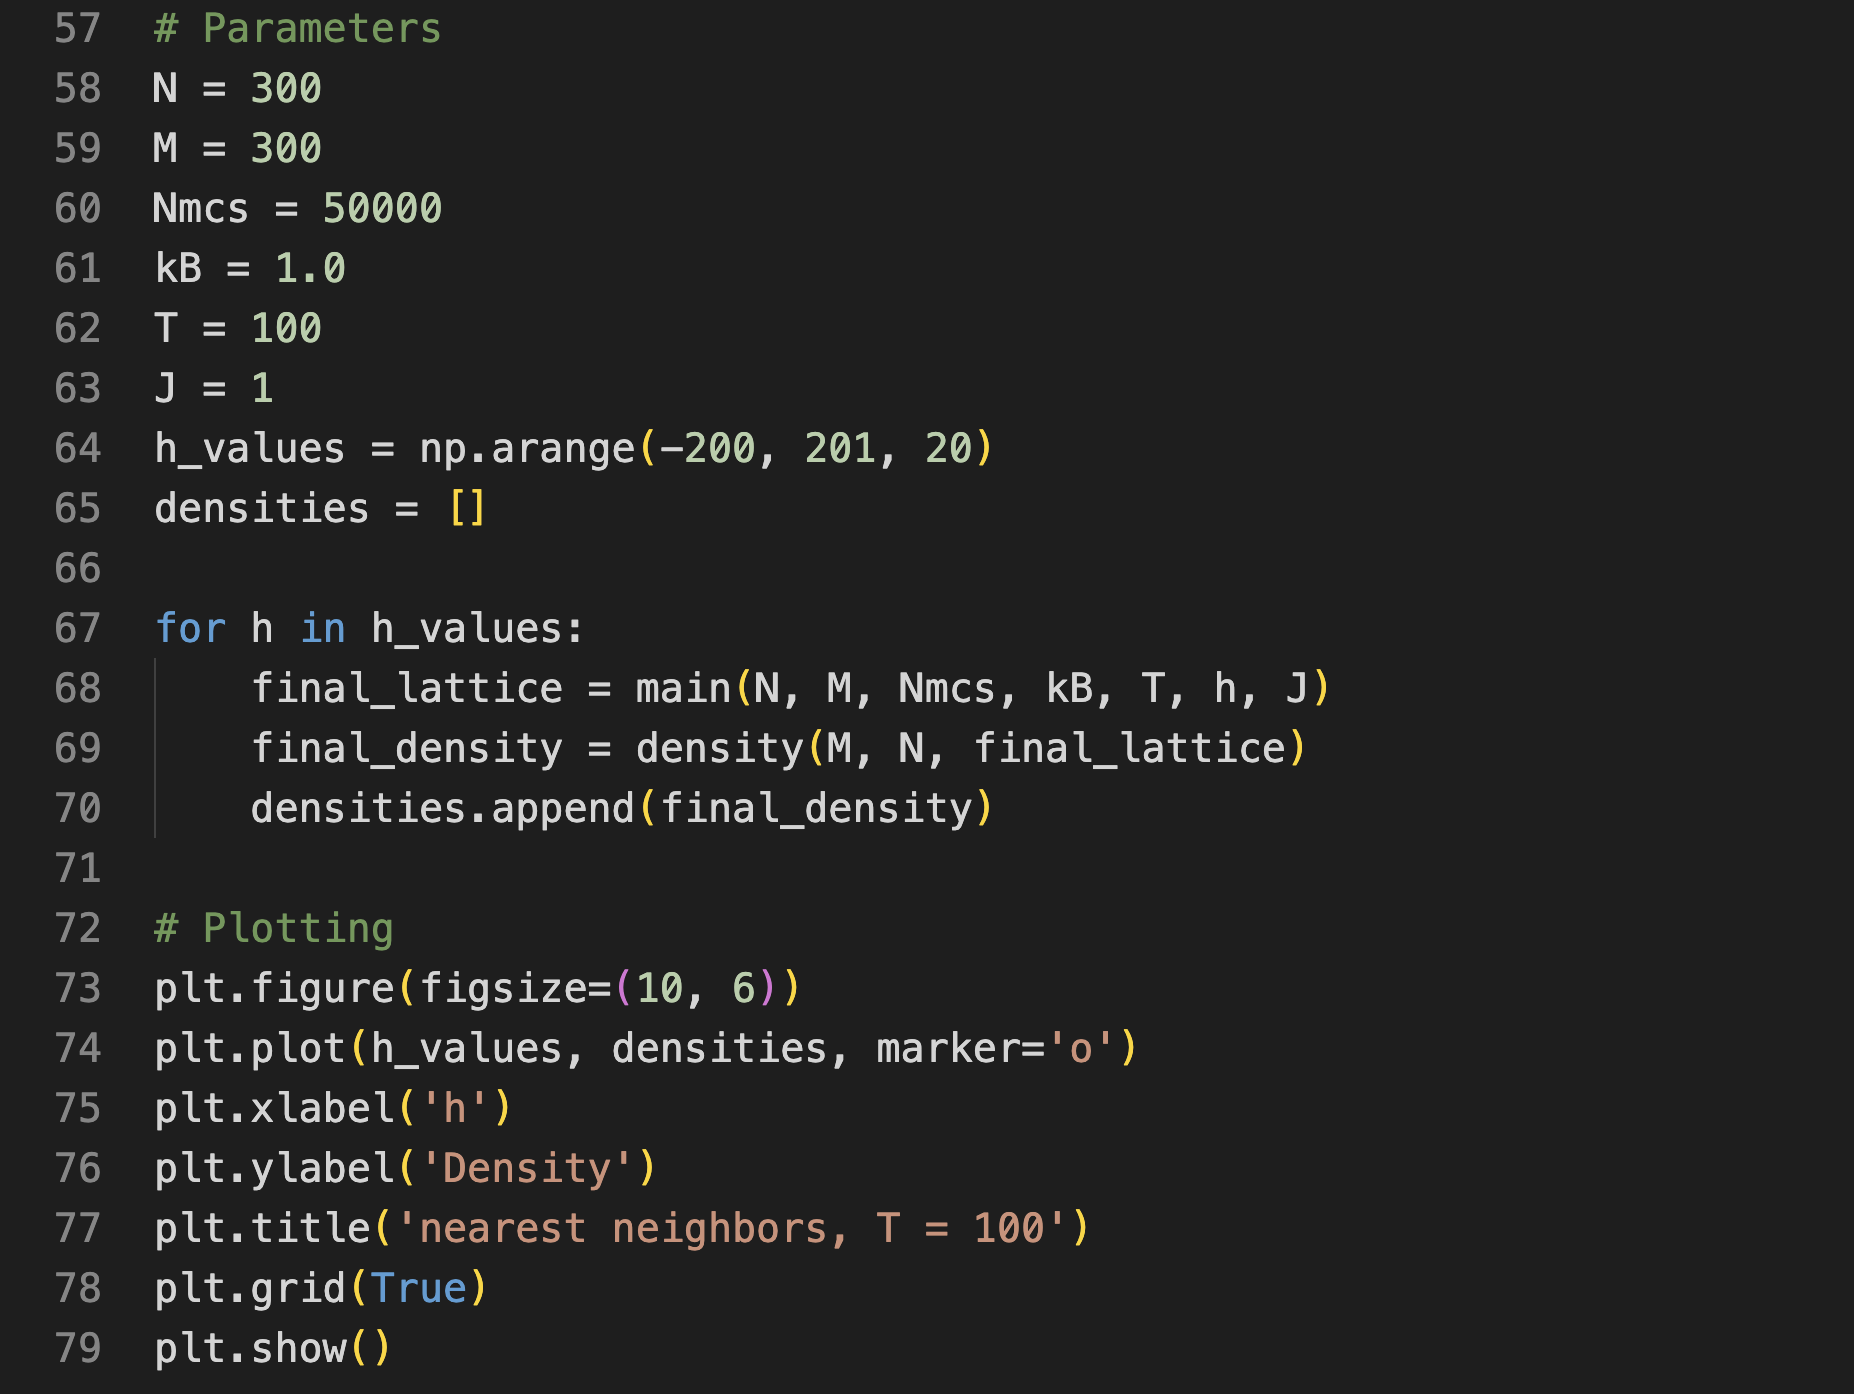
\includegraphics[width=1\linewidth]{nn_callingtheFunctions.png}
    \caption{Calling the functions}
    \label{fig45}
\end{figure}

\section{The Long-Range Model}

Unlike the nearest-neighbors model, we no longer assume that the selected point can only be affected by its four nearest neighbors. In the long-range model, we let the selected point have some sort of relationship with all the other points in the lattice. However, among these points, some may be very close to the selected point, while others are very far away, and it doesn't make sense if all the points have the same degree of influence. Thus, we want to introduce a parameter 
\[
J = \frac{1}{(\left| x_1 - y_1 \right| + \left| x_2 - y_2 \right|)^a}
\]
which ensures that the closer two points are, the bigger the influence will be. In this expression, $(x_1, x_2)$ is the selected point and $(x_2, y_2)$ is a point in the lattice. $\left| x_1 - y_1 \right| + \left| x_2 - y_2 \right|$ is the distance between the two points, which can also be counted by the number of grid sides between them. $a$ is a constant that when it is a big number, the overall influence will be reduced, and when it is a small number, the overall influence will be enhanced. And now, we are well prepared to calculate the Hamiltonian.

\begin{figure}
    \centering
    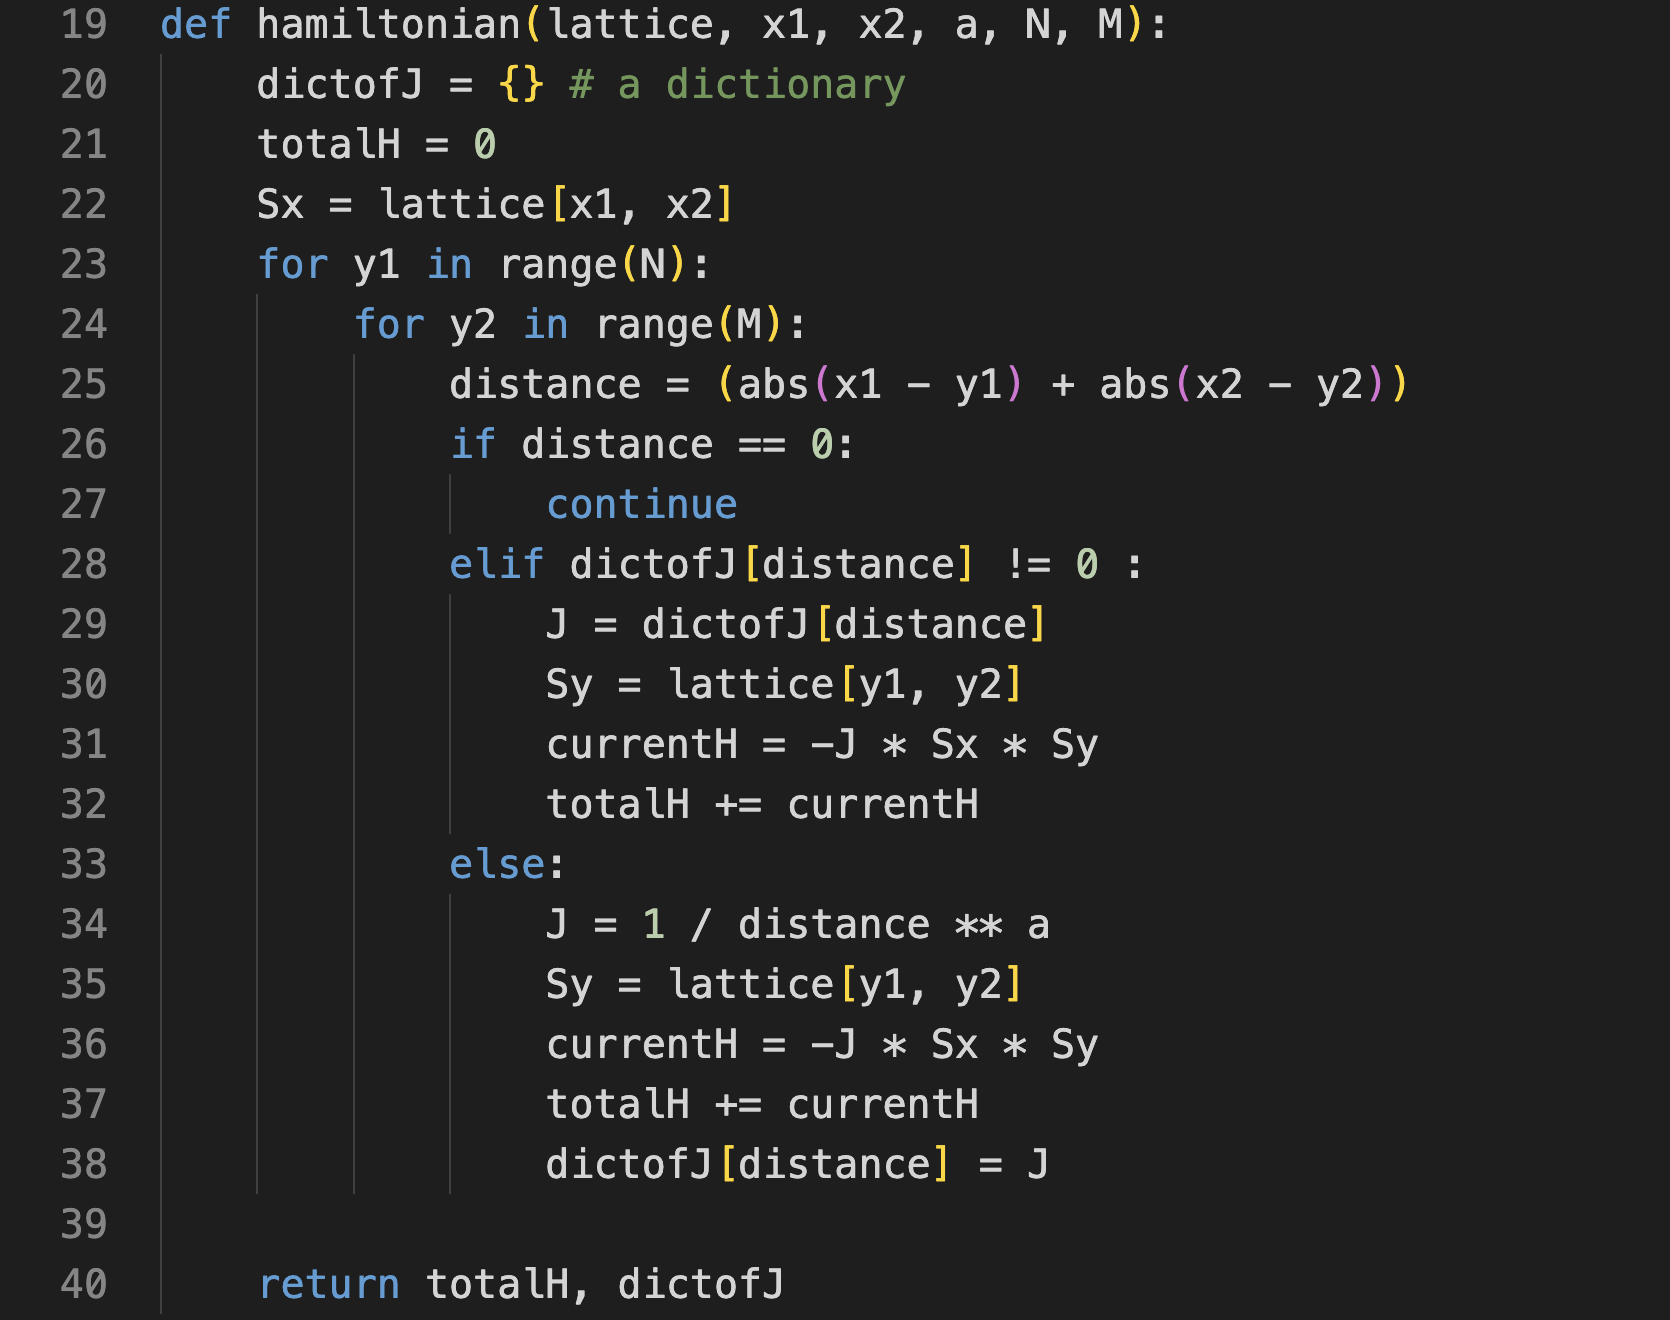
\includegraphics[width=1\linewidth]{lr_hamiltonian.png}
    \caption{\texttt{hamiltonian(lattice, x1, x2, a, N, M)}}
    \label{fig46}
\end{figure}

\subsection{\texttt{hamiltonian(lattice, x1, x2, a, N, M)}}

From the section above, we may realize that for all different combinations of the points, as long as the distance between the two points is the same, $J$ is the same. If we calculate $J$ separately in each iteration, there will be a lot of unnecessary repetitions making the algorithm very time-costly. Therefore, we first create a dictionary in which the keys cover all the possibilities of the distances, and the values are the corresponding $J$. Then in each iteration, if the distance can be found in the keys, we can use its $J$ directly. If the distance is new to the dictionary, then we have no choice but to calculate the $J$ first, and add this key-value pair to the dictionary. Next, Let's recall the formula for calculating the 
\[
H_{\Lambda}(\sigma) = -  \sum_{x,y\in \Lambda}\frac{1}{(\left| x_1 - y_1 \right| + \left| x_2 - y_2 \right|)^a}\sigma_x \sigma_y.
\]
In this expression, $\sigma_x$ and $\sigma_y$ are equal to $S_x$ and $S_y$\, respectively, in the codes. Therefore, in each iteration, we calculate the current Hamiltonian by $currentH = -J \cdot S_x \cdot S_y$. Then we add the currentH to the totalH. Finally, after iterating through all the points in the lattice, we get the total Hamiltonian. 

\subsection{\texttt{main(N, M, Nmcs, kB, T, a, h)}}

The main function of the long-range model is very similar to that of the nearest-neighbors model. As we did before, we first generate a random lattice where each point is either $1$ or $-1$. Next, we write an outer iteration which counts the times of the Monte Carlo process. Then in each iteration, we randomly select a point in the graph. If $S = -1$ and the sum of its nearest neighbors is bigger than -4, we follow the metropolis algorithm to decide whether or not to flip the value of $S$. If the sum is -4, we keep the value of S. In the other case, if $S = 1$, we follow the metropolis algorithm with border conditions. Finally, after the times of the Monte Carlo process reach $Nmcs$, we return the final lattice.

\begin{figure}
    \centering
    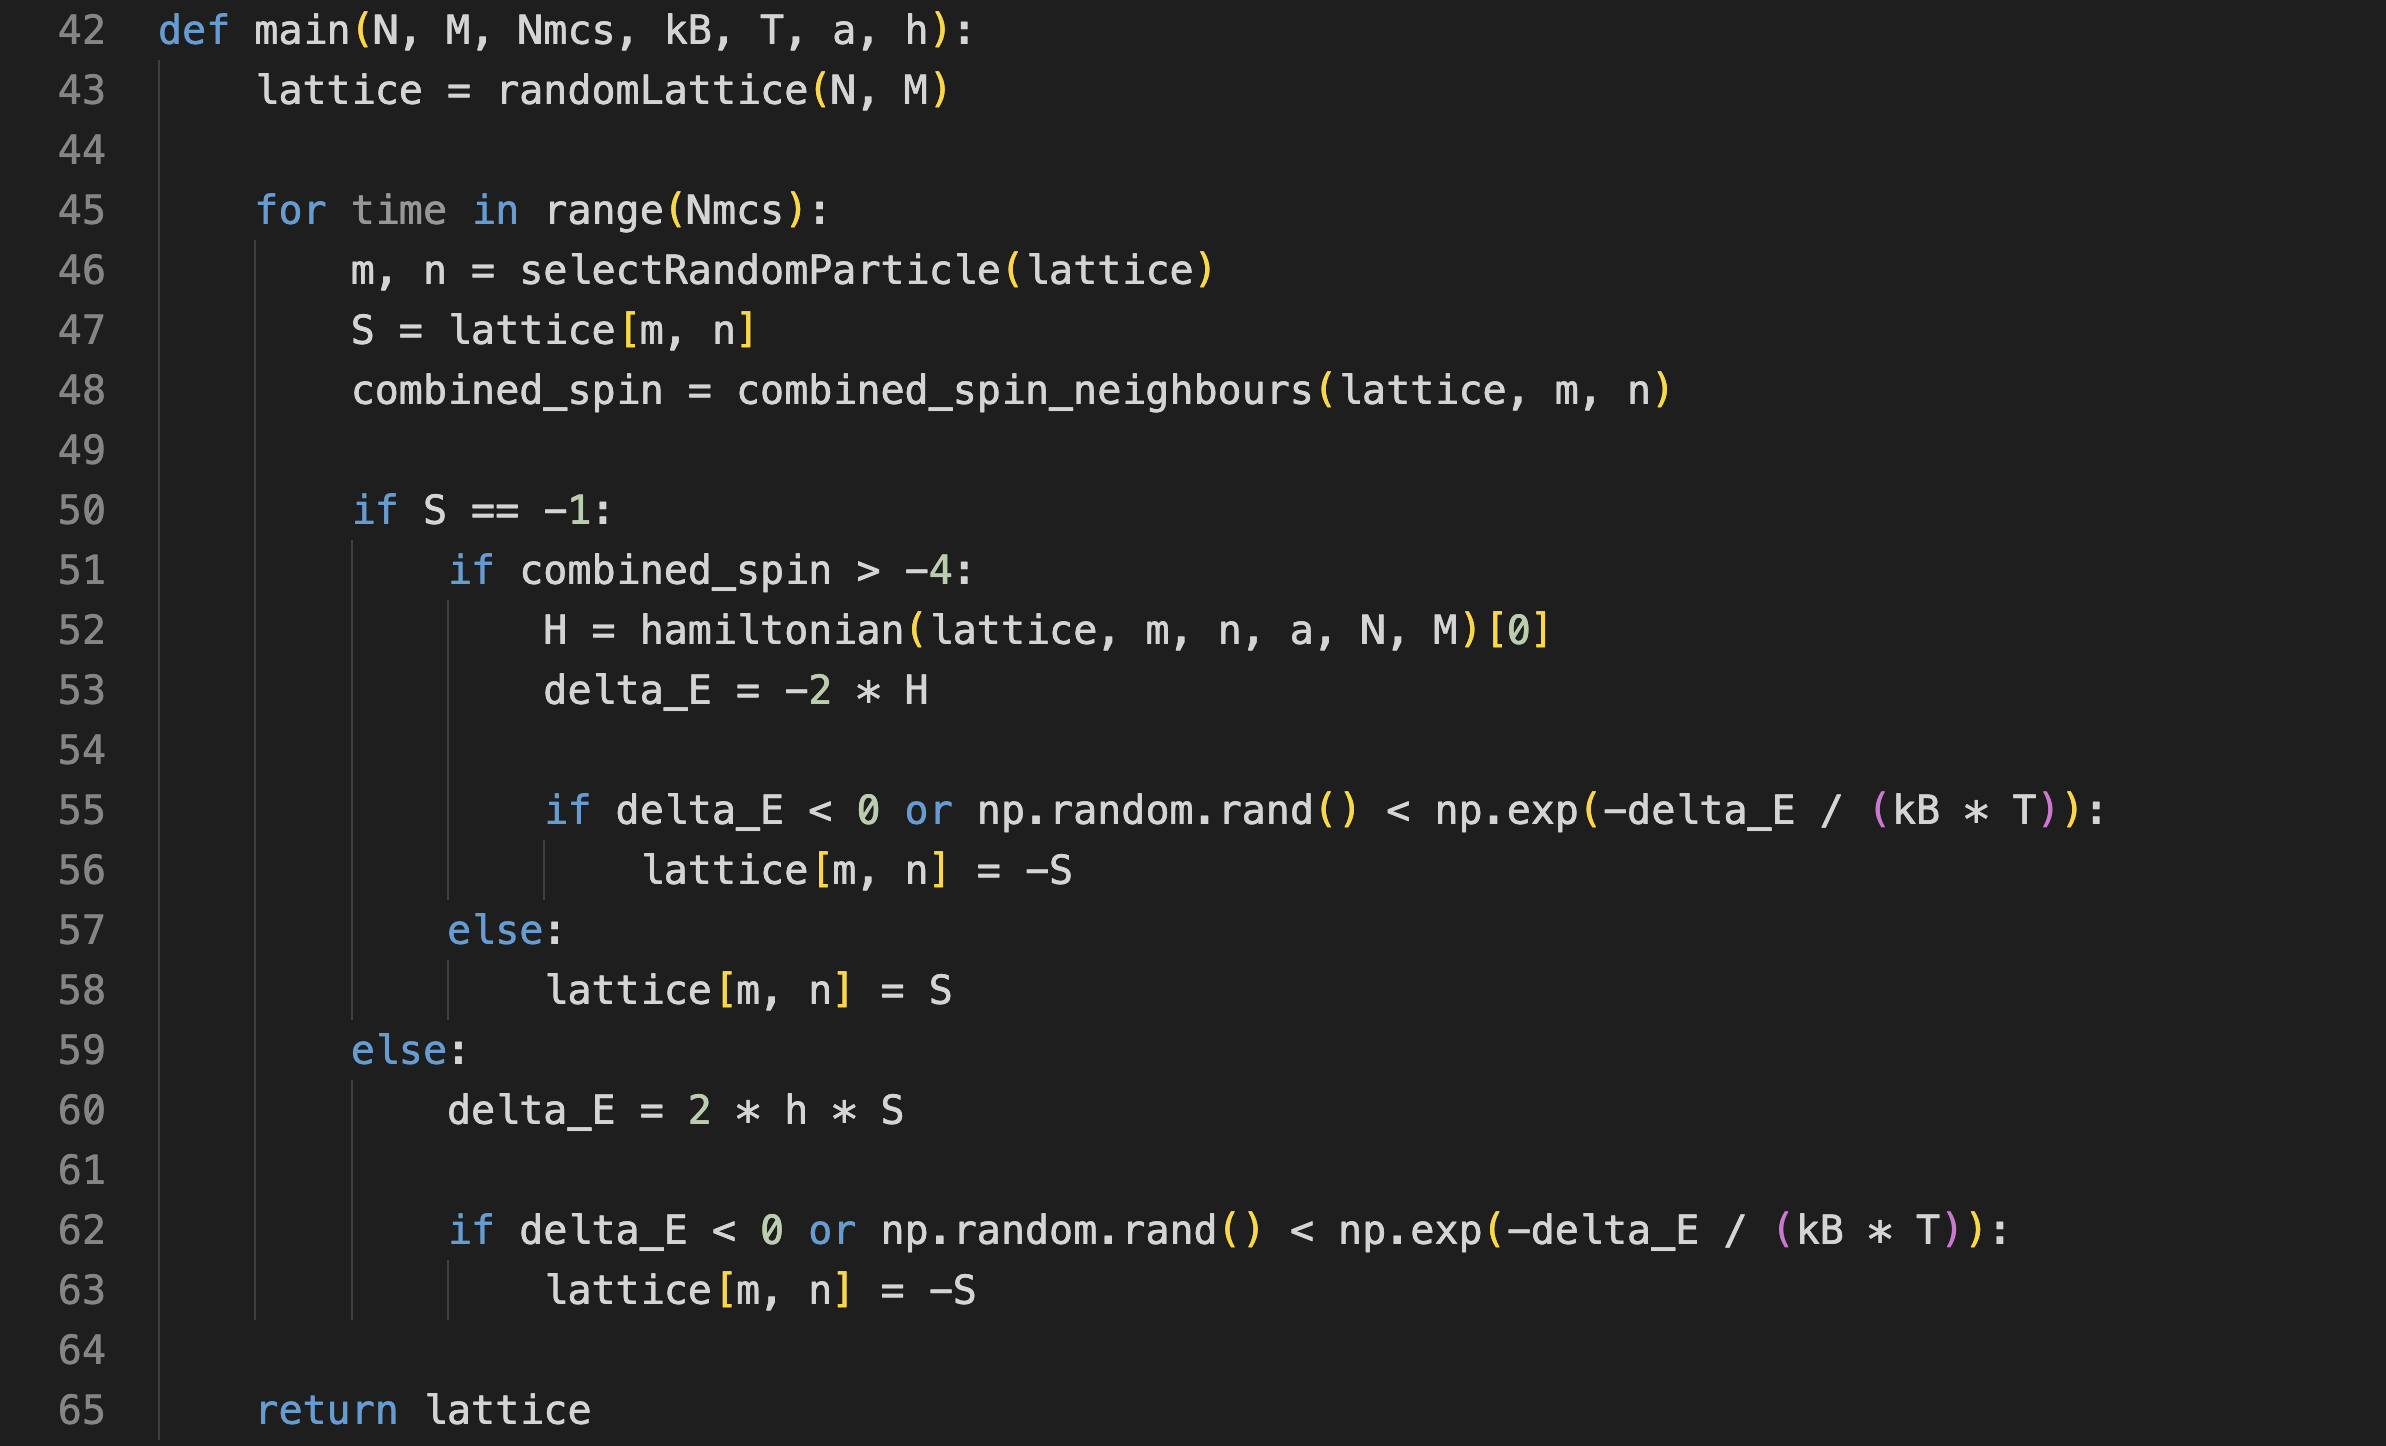
\includegraphics[width=1\linewidth]{lr_main.png}
    \caption{\texttt{main(N, M, Mmcs, kB, T, a, h)}}
    \label{fig47}
\end{figure}

\section{The Random-Graph Model}

The random-graph model is quite different from the previous two models. In both the nearest-neighbors model and the long-range model, we put the points in an $N \times M$, $2D$ grid. But in the random-graph model, we want to generate points that are randomly distributed on a plane. For any different two points, or more often called vertices, they can either be connected with a line, which we call an edge, or not connected at all. It is important to notice that a vertex is not allowed to connect with itself. From the graph, we can create a matrix recording all the information needed to draw the graph, which is usually named as the incident matrix. Let's assume that there are altogether $n$ vertices in the graph. Correspondingly, we can create an $n \times n$ incident matrix. The entry $(i, j)$ represents the number of edges between vertex $i$ and vertex $j$. If the number is 0, $i$ and $j$ are not connected. Otherwise, they are connected. Now consider that we want to travel from vertex $i_0$ to vertex $i_i$. There can be many combinations of routes depending on the graph. We define the total amount of these possible routes as the walks, and the number of edges covered in each route as the length. 

\subsection{\texttt{generateIncidentMatrix(n, p)}}
In our code, we would like to skip the procedure of drawing the graph and instead, directly generate the incident matrix. The entries of it have the possibility of $1-p$ to be $0$ and the possibility of $p$ to be $1$. However, since a vertex is not allowed to connect with itself, we need to change all the entries on the long diagonal, which are $(0, 0), (1, 1), \ldots, (n, n)$, to be $0$.

\begin{figure}
    \centering
    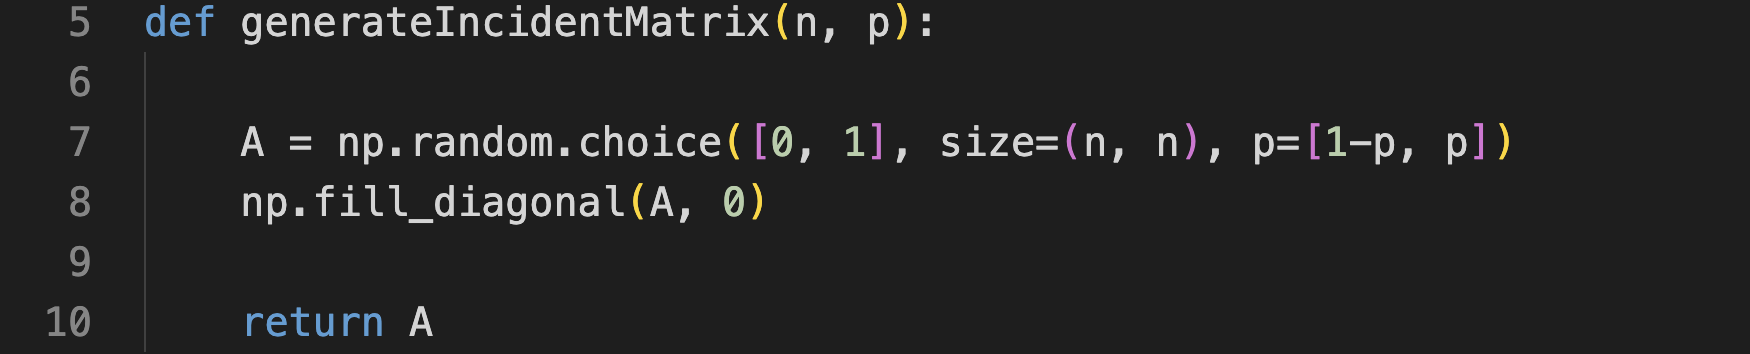
\includegraphics[width=1\linewidth]{rg_generateIncidentMatrix.png}
    \caption{\texttt{generateIncidentMatrix(n, p)}}
    \label{fig48}
\end{figure}

\subsection{\texttt{generatePhysicalCondition(n)}}
There are n vertices in total. We want to randomly assign each vertex with $-1$ and $1$, which represent being healthy and being ill respectively.

\begin{figure}
    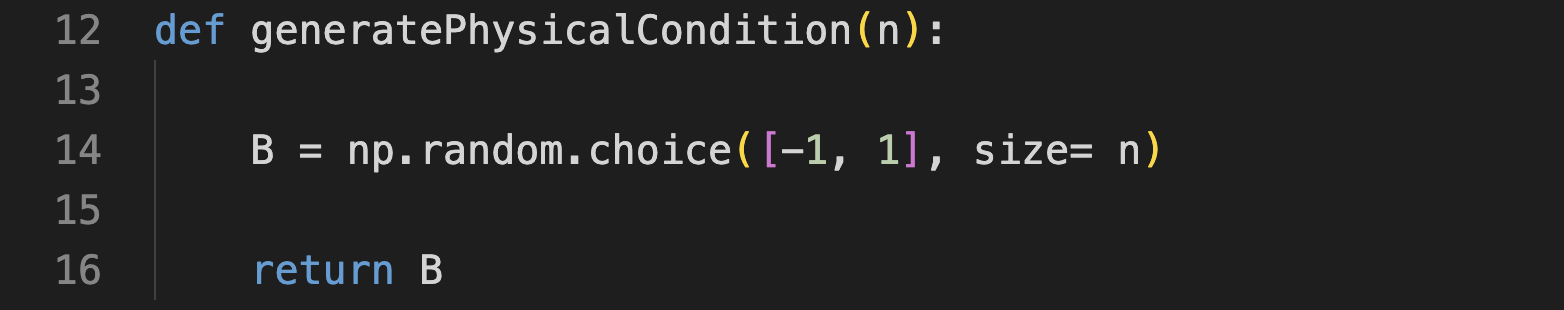
\includegraphics[width=1\linewidth]{rg_generatePhysicalCondition.png}
    \caption{generatePhysicalCondition(n)}
    \label{fig49}
\end{figure}

\subsection{\texttt{totalWalks(A, k)}}
In fact, we have a formula to calculate the walks from vertex $i$ to vertex $j$ with length m \cite{Bol},
\[
walks = A^m[i, j].
\]
Therefore, the total walks from $i$ to $j$ with lengths ranging from $1, 2,..., k$ should be:
\[
totalWalks = \left(\sum_{m = 1}^{k} A^m \right)[i, j].
\]
Following this formula, we can naturally write the code for totalWalks. Note that in order to calculate $A^m$, we need to use the Python built-in function \texttt{np.linalg.matrix\_power(A, m)}.

\begin{figure}
    \centering
    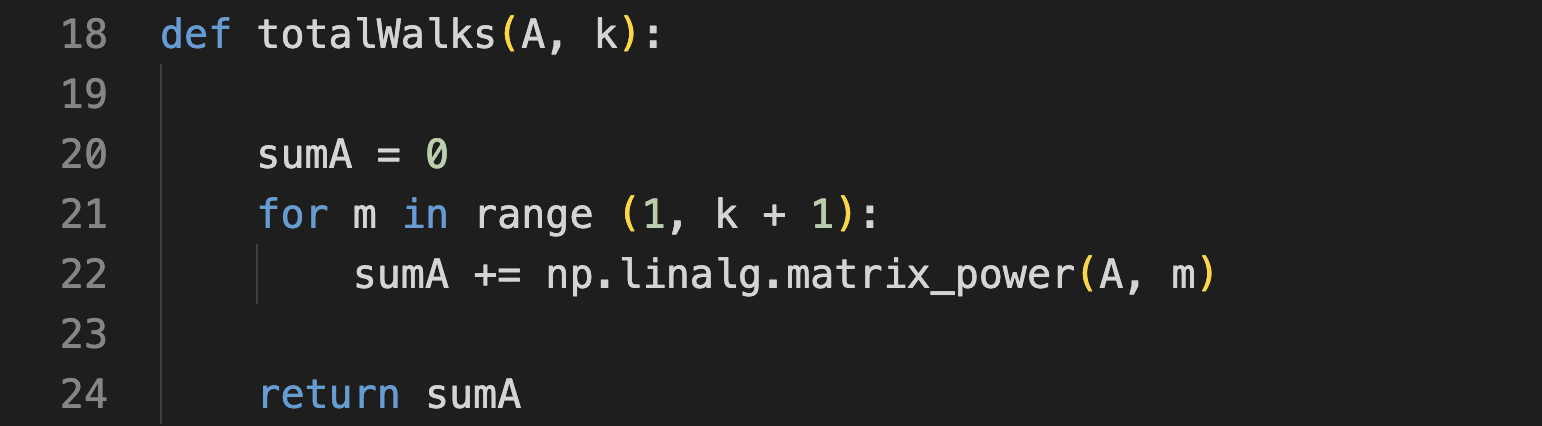
\includegraphics[width=1\linewidth]{rg_totalWalks.png}
    \caption{totalWalks(A, k)}
    \label{fig50}
\end{figure}

\subsection{\texttt{hamiltonian(sumA, B, n)}}
Let's adapt the formula for calculating the Hamiltonian in the long-range model into
\[
H = -\sum_{i, j} \left( (\sum_{m = 1}^{k} A^m)[i, j] \right) \sigma_i \sigma_j.
\]
In each iteration, we follow the formula to get the Hamiltonian in that iteration, then add it to the total Hamiltonian. After iterating over all the entries in the incident matrix, we get the total Hamiltonian.

\begin{figure}
    \centering
    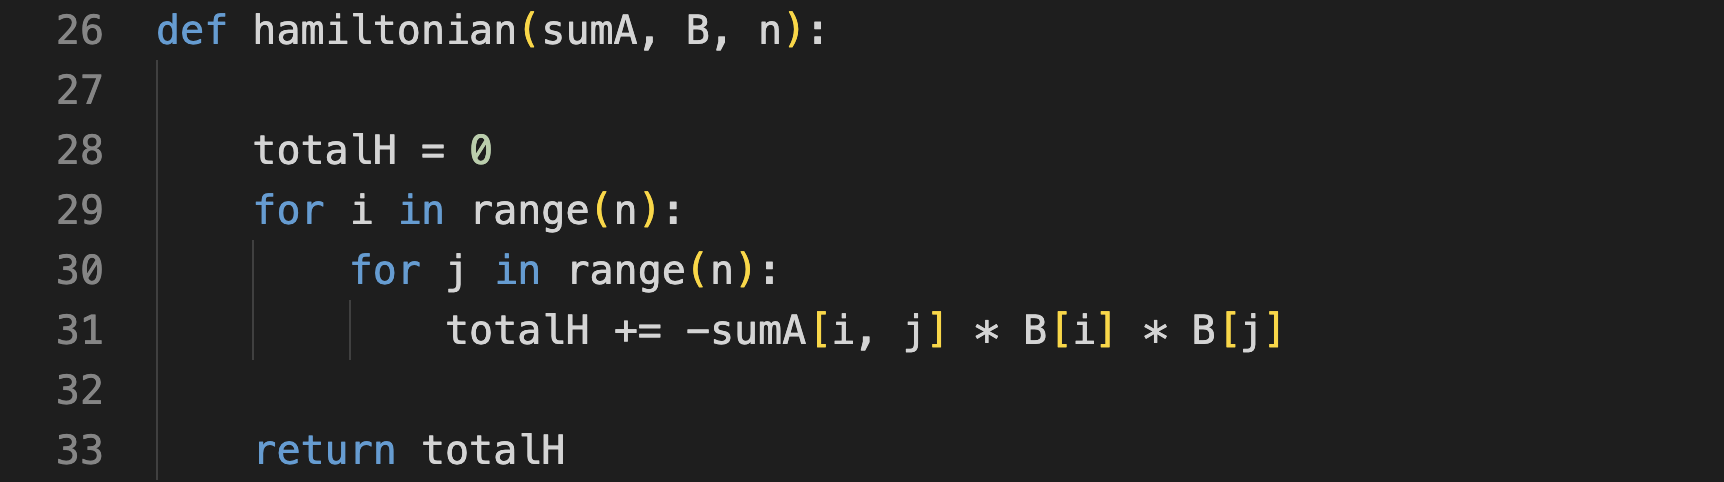
\includegraphics[width=1\linewidth]{rg_hamiltonian.png}
    \caption{\texttt{hamiltonian(sumA, B, n)}}
    \label{fig51}
\end{figure}

\subsection{\texttt{selectRandomParticle(lattice)}}
In this model, we have $n$ points in total. We have already put them in an $1 \times n$ matrix in the function \texttt{generatePhysicalCondition(n)}, where each point can be represented by the ordered pair $(0, i)$. Therefore, when we select one point randomly, we only need to generate a random integer $i \in [0, n]$

\begin{figure}
    \centering
    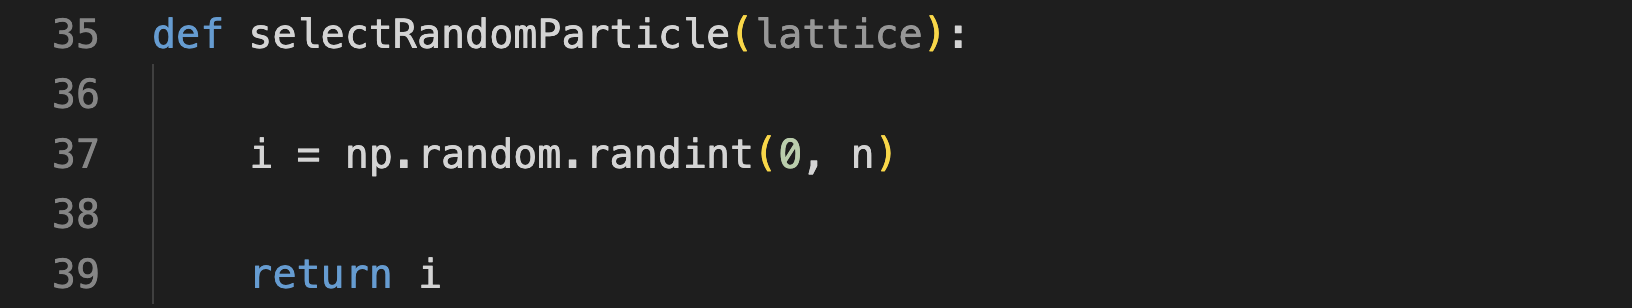
\includegraphics[width=1\linewidth]{rg_selectRandomParticle.png}
    \caption{\texttt{selectRandomParticle(lattice)}}
    \label{fig52}
\end{figure}

\subsection{\texttt{main(n, B, sumA, T, h, Nmcs, kB)}}
Similar to the nearest-neighbors model and the long-range model, we first write an outer iteration counting the times of the Monte Carlo process. Then in each iteration, we randomly select a point in the graph. $S$ is the value of the point. If $S = -1$, we follow the metropolis algorithm to decide whether or not to flip the value of $S$. If $S = 1$, we follow the metropolis algorithm with border conditions. Finally, after the times of the Monte Carlo process reach $Nmcs$, we return the final lattice.

\begin{figure}
    \centering
    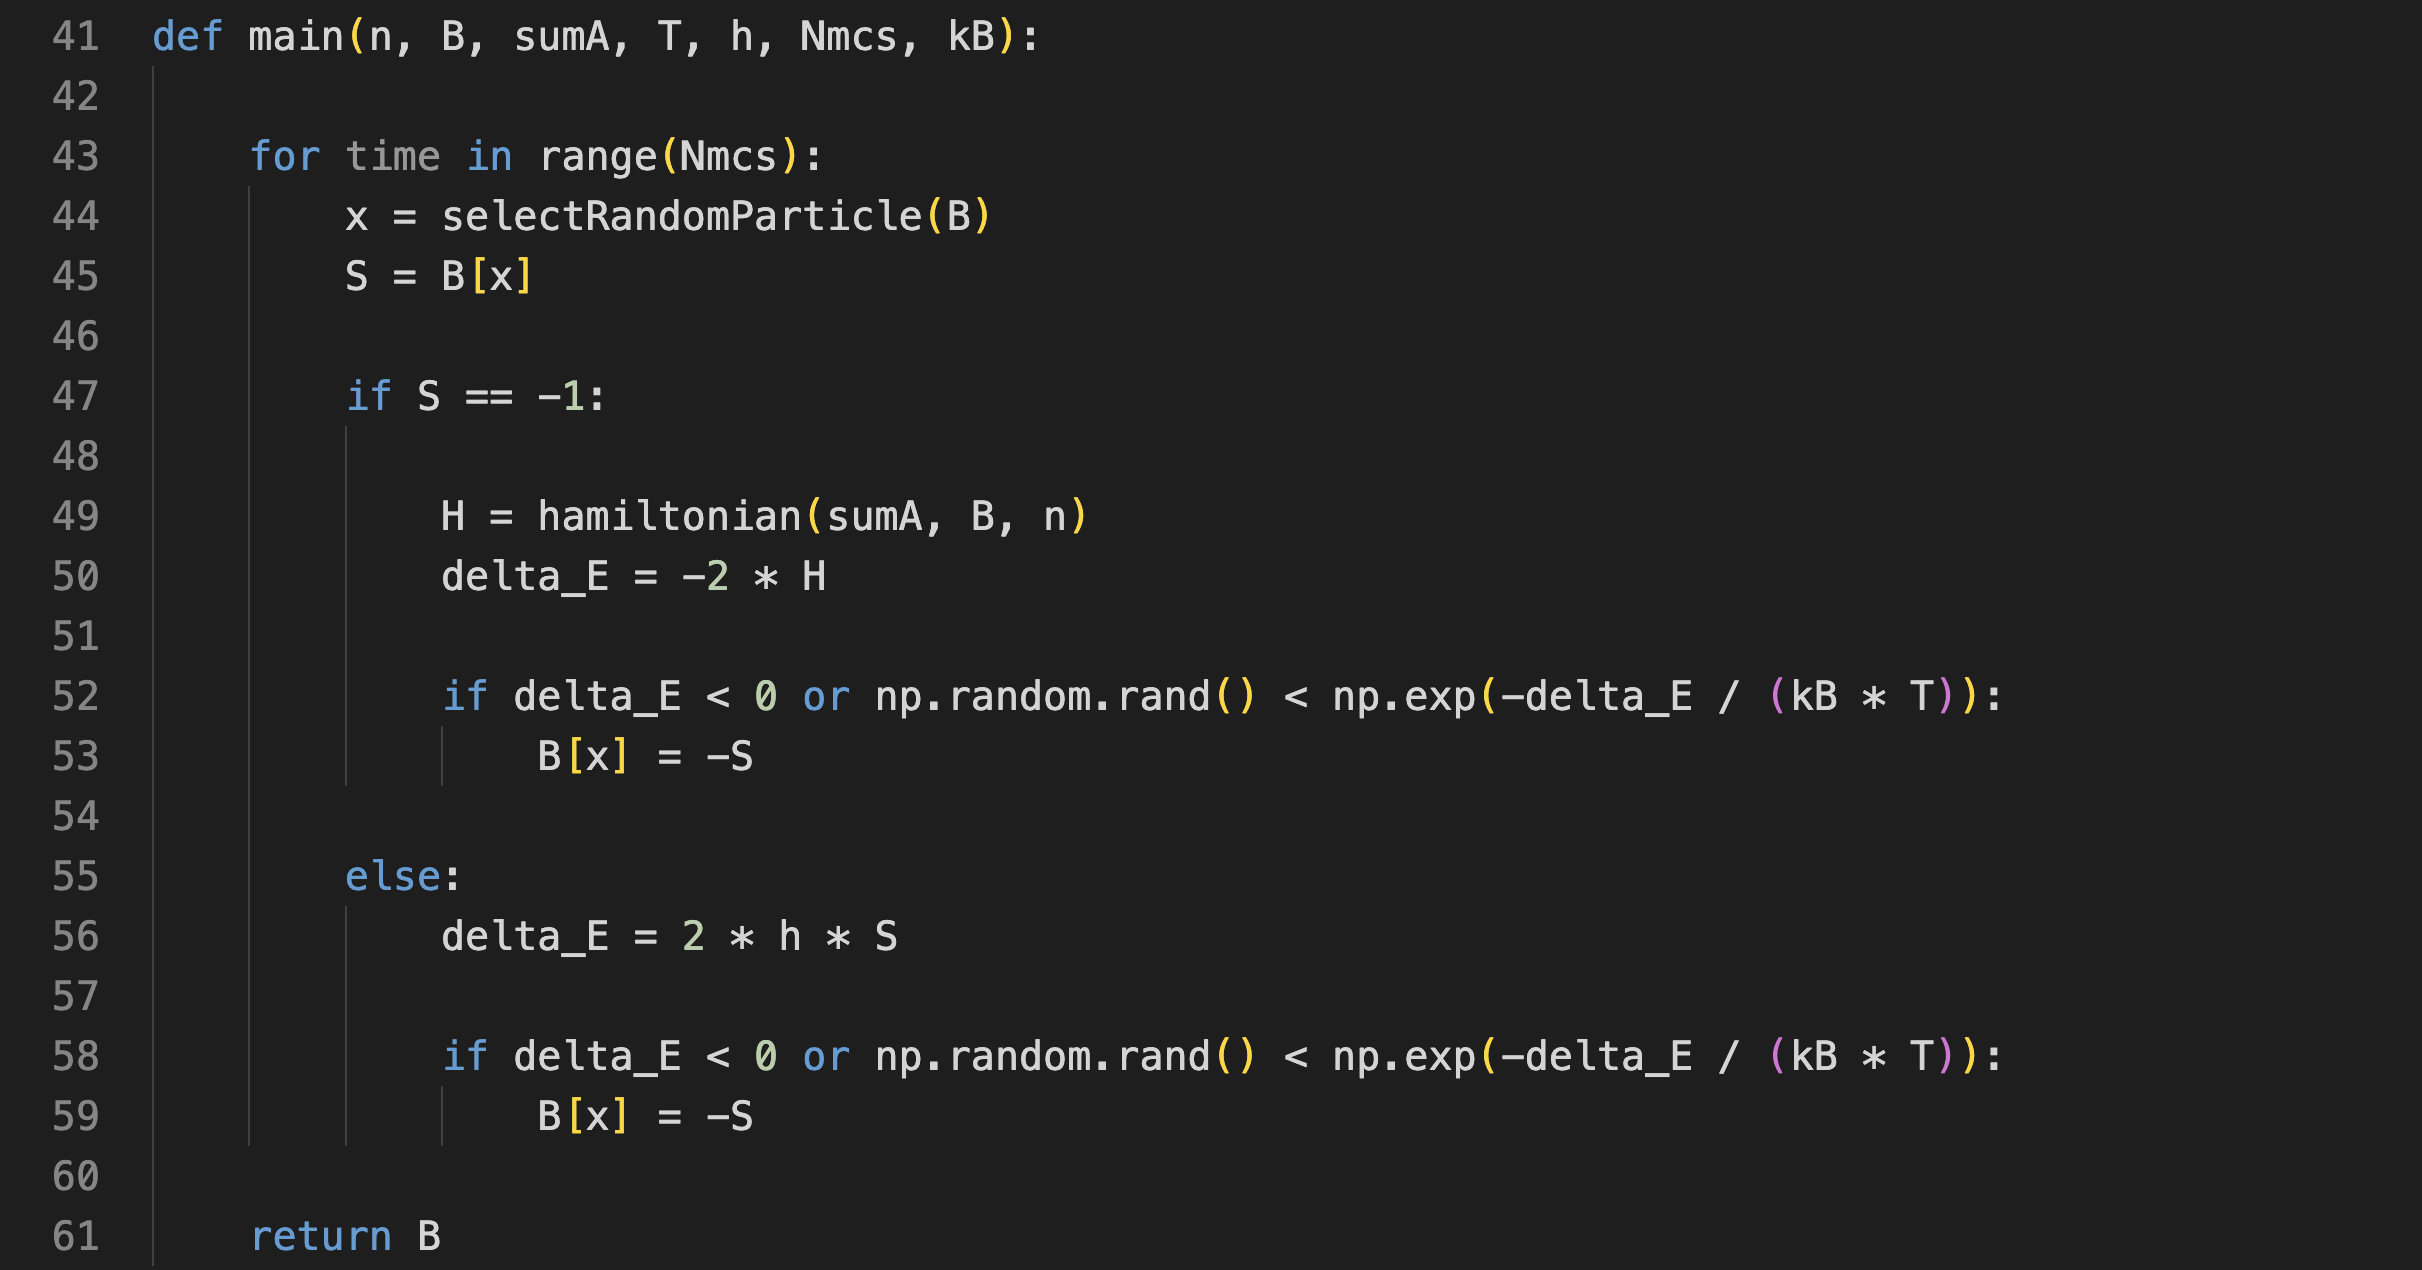
\includegraphics[width=1\linewidth]{rg_main.png}
    \caption{\texttt{main(n, B, sumA, T, h, Nmcs, kB)}}
    \label{fig53}
\end{figure}

\subsection{Calling the Functions}
First, we generate a random graph and assign each point with either $1$ or $-1$. We also calculate the total walks ahead of time. Then we call the main function and get the final lattice. Finally, based on the final conditions of these $n$ points, we can calculate the density of infected people, and draw the graph showing its relationship with different values of $h$.

\begin{figure}
    \centering
    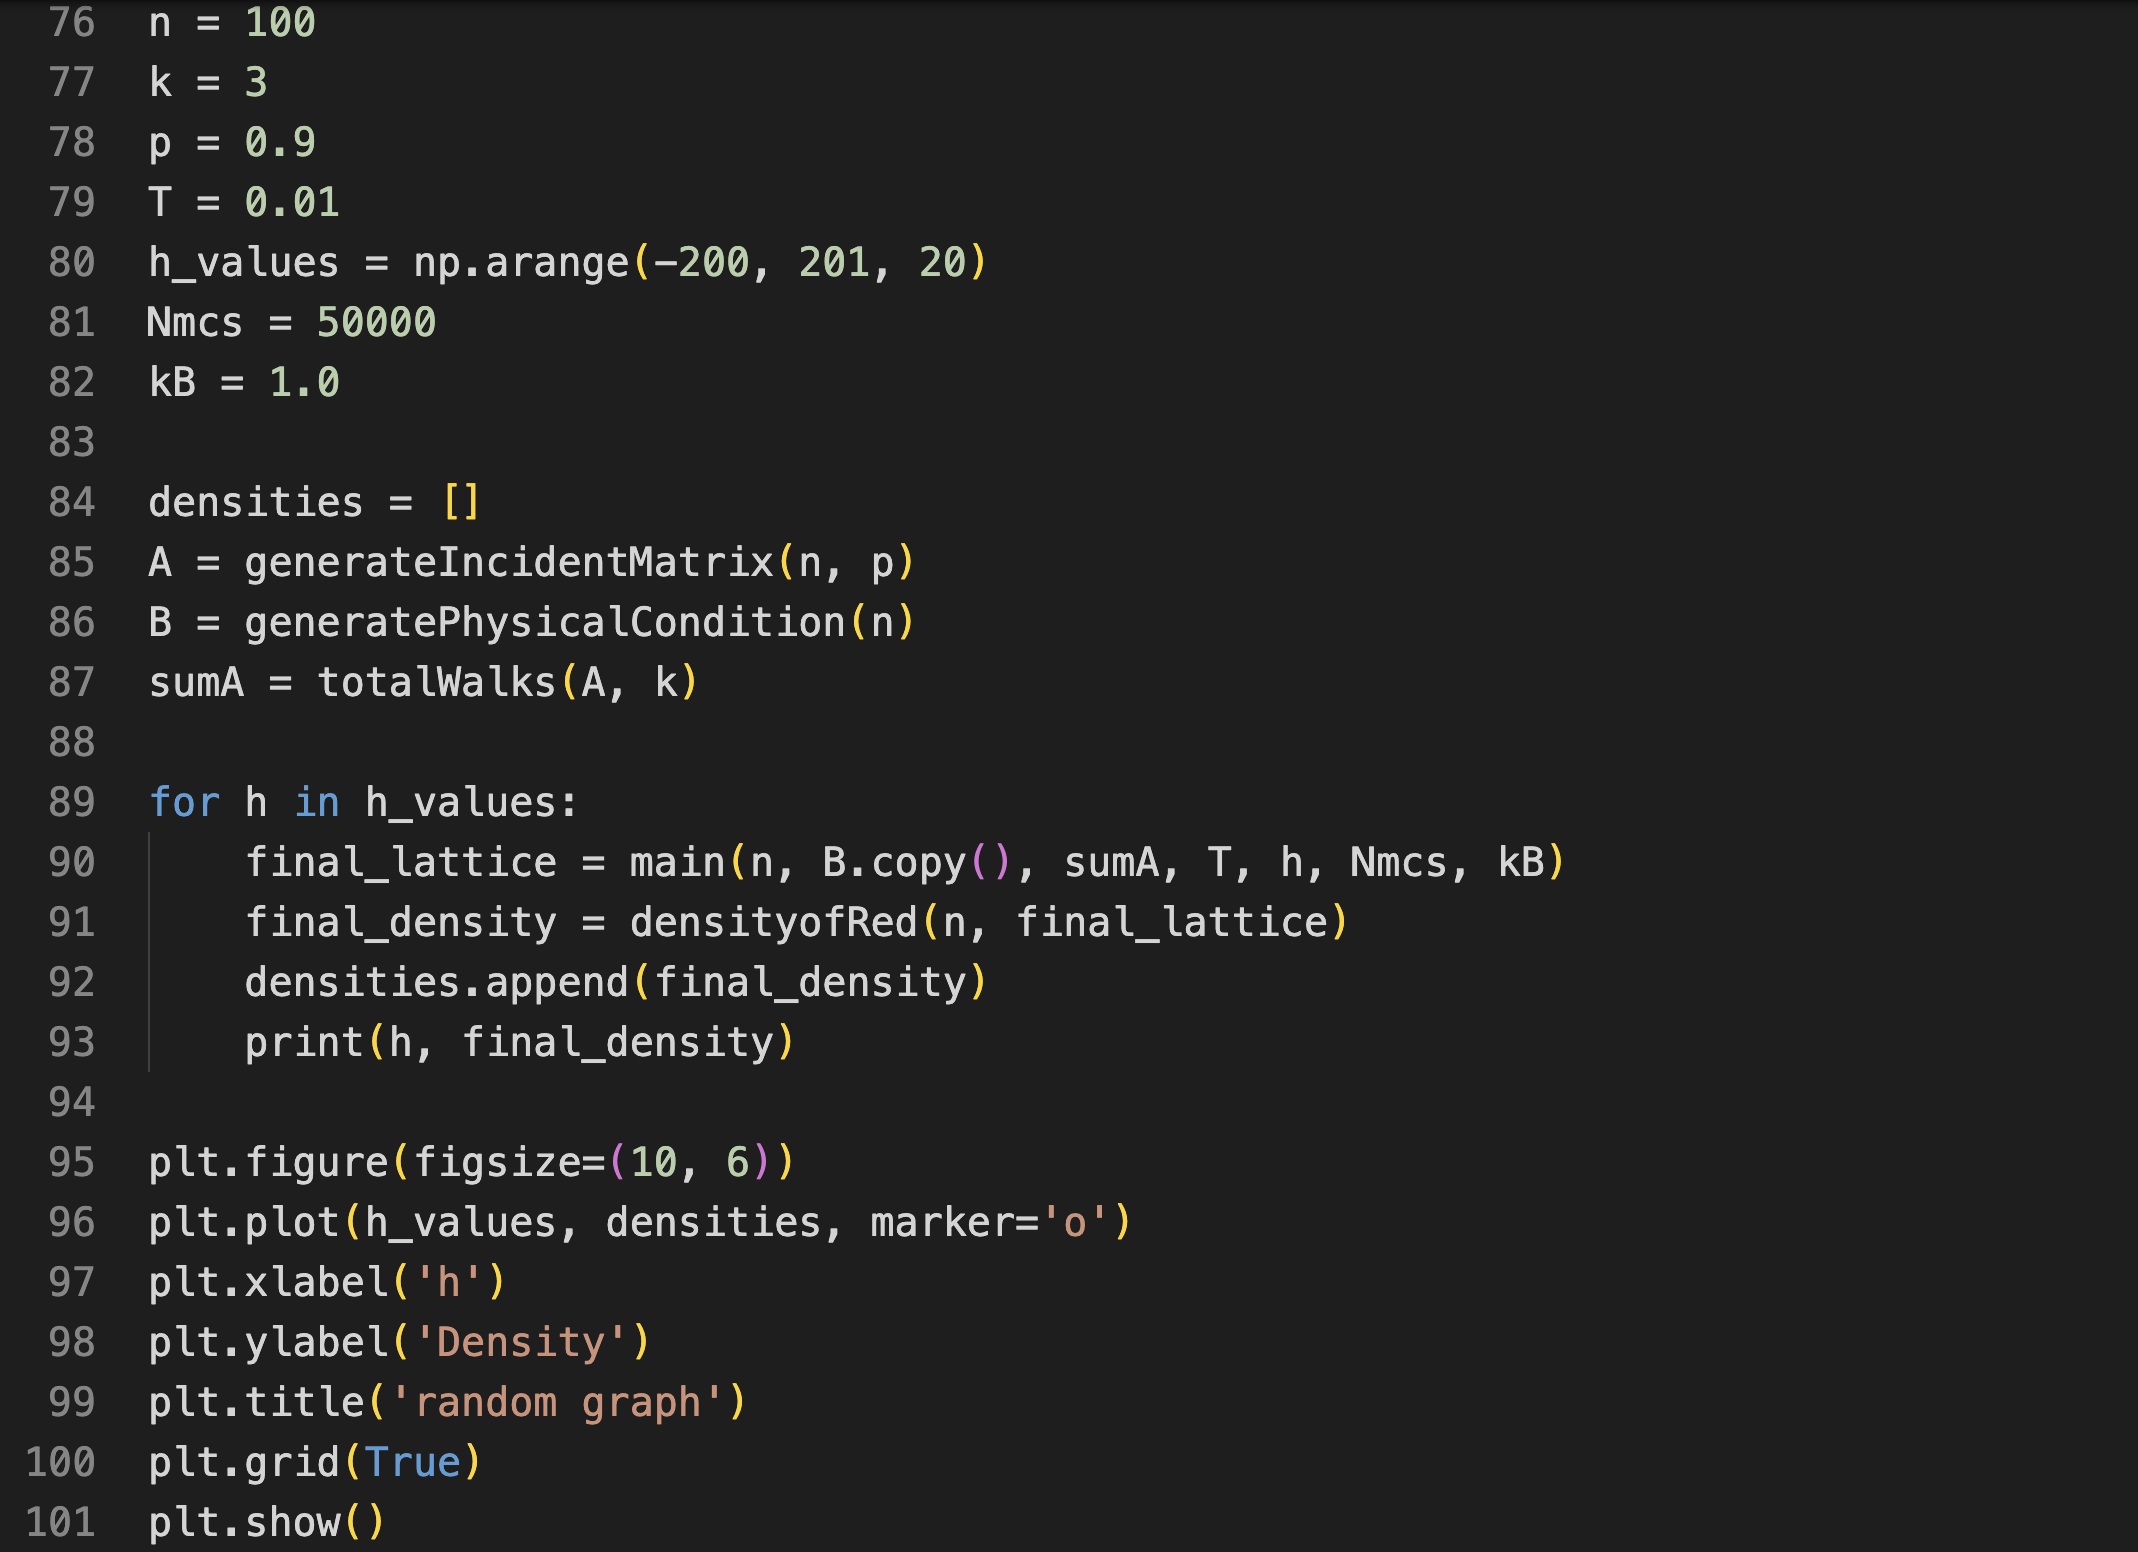
\includegraphics[width=1\linewidth]{rg_callingtheFunctions.png}
    \caption{Calling the functions}
    \label{fig54}
\end{figure}

\chapter{Summary}
\markboth{Summary}{}

In this chapter, we summarize the findings of our study, which integrates concepts from Statistical Mechanics and mathematical modeling to explore the dynamics of infection spread. Our project began by adapting the Ising model—a fundamental tool in Statistical Mechanics used to study phase transitions in magnetic systems—to analyze the relationship between spatial distance and infection probability.

We developed three distinct infection models: the nearest-neighbors model, the long-range interaction model, and the random-graph model. These models provide different perspectives on how infections propagate through populations: Nearest-Neighbors Model focuses on infection spread within close proximity, resembling local transmission scenarios; Long-Range Interaction Model accounts for infections that occur over greater distances, highlighting the importance of mobility and migration patterns in disease dynamics; Random-Graph Model introduces randomness into the distribution of people, allowing us to study more complex and less predictable transmission networks. Each model was analyzed with particular attention given to how varying parameters, such as infection rates and initial conditions, affect the spread of disease. We applied both one-dimensional and two-dimensional simulations to observe infection patterns and transitions to equilibrium states.

In conclusion, this project has applied mathematical concepts to provide inspirations for the real-life infection problem. The interdisciplinary approach, combining insights from Physics, Mathematics, and Computer Science, has not only enhanced our understanding of infection spread but also demonstrated the power of collaborative research in solving complex problems.


\chapter{Acknowledgements}
\markboth{Acknowledgements}{}
\noindent

This Summer Project is supported by Deans' Undergraduate Research Fund (DURF), NYU Shanghai.

We would like to express our deepest gratitude to Professor Endo, for his invaluable guidance and support throughout this research. His insightful comments and constructive feedback greatly enhanced the quality of this work. Special thanks to his patience and encouragement in the whole process, no matter in the mini lectures offline or meeting online, which makes it possible for three freshmen to finish their first academic research in three months. 

We also wish to acknowledge our families and friends for their unwavering support and encouragement throughout the summer. Their belief in our abilities kept us motivated and focused.

Lastly, we thank everyone whose support made this DURF project possible.

\begin{thebibliography}{9}
\bibitem{Bamidele} \url{https://cocalc.com/share/public_paths/bb76377ee6823f7155a629e6f072f30d7c0b956f}
\bibitem{Bol} B. Bollob\'{a}s. Modern Graph Theory. Graduate Texts in Mathematics 184 Springer-Verlag New York, 1 edition, 1998.
\bibitem{curve}\url{https://mycurvefit.com/}
\bibitem{dys} F.J. Dyson. Existence of a Phase Transition in a One-Dimensional Ising ferromagnet. {\em Communications in Mathematical Physics.} {\em 12}: 91--107, 1969.
\bibitem{ER} P. Erd\H{o}s, A. R\'{e}nyi. On Random Graphs I. Publicationes Mathematicae, {\bf 6}: 290--297,  1959.
\bibitem{FV} S. Friedli, Y. Velenik. Statistical Mechanics of Lattice Systems: A Concrete Mathematical Introduction. Cambridge University Press, Cambridge, 2017.
\bibitem{frsp} J. Fr\"ohlich, T. Spencer. The phase transition in the one-dimensional Ising model with $1/r^2$ interaction energy. {\em Communications in Mathematical Physics.} {\bf 84}:87--101, 1982.
\bibitem{HOG} H.O. Georgii. {\em Gibbs Measures and Phase Transitions}. De Gruyter Studies in Mathematics, Vol 9, Berlin--New York, 1988, 2nd Edition 2011.
\bibitem{Ising} E. Ising. Beitrag zur Theorie des Ferromagnetismus. Zeitschrift für Physik. {\bf 31}: 253--258, 1925.
\bibitem{LY}
T.D. Lee and C.N. Yang. {\it Statistical Theory of Equations of State and Phase Transitions II. Lattice Gas and Ising Model}. \emph{Phys. Rev.} \textbf{87}, 404--409, 1952.
\bibitem{Peierls} R. Peierls. On Ising's model of ferromagnetism. {\em Proceedings of the Cambridge Philosophical Society}, \textbf{32}, 477-481, 1936.
\end{thebibliography}



\end{document}